% Options for packages loaded elsewhere
\PassOptionsToPackage{unicode}{hyperref}
\PassOptionsToPackage{hyphens}{url}
%
\documentclass[
  11pt,
  man,mask,floatsintext]{apa6}
\usepackage{amsmath,amssymb}
\usepackage{iftex}
\ifPDFTeX
  \usepackage[T1]{fontenc}
  \usepackage[utf8]{inputenc}
  \usepackage{textcomp} % provide euro and other symbols
\else % if luatex or xetex
  \usepackage{unicode-math} % this also loads fontspec
  \defaultfontfeatures{Scale=MatchLowercase}
  \defaultfontfeatures[\rmfamily]{Ligatures=TeX,Scale=1}
\fi
\usepackage{lmodern}
\ifPDFTeX\else
  % xetex/luatex font selection
\fi
% Use upquote if available, for straight quotes in verbatim environments
\IfFileExists{upquote.sty}{\usepackage{upquote}}{}
\IfFileExists{microtype.sty}{% use microtype if available
  \usepackage[]{microtype}
  \UseMicrotypeSet[protrusion]{basicmath} % disable protrusion for tt fonts
}{}
\makeatletter
\@ifundefined{KOMAClassName}{% if non-KOMA class
  \IfFileExists{parskip.sty}{%
    \usepackage{parskip}
  }{% else
    \setlength{\parindent}{0pt}
    \setlength{\parskip}{6pt plus 2pt minus 1pt}}
}{% if KOMA class
  \KOMAoptions{parskip=half}}
\makeatother
\usepackage{xcolor}
\usepackage{longtable,booktabs,array}
\usepackage{calc} % for calculating minipage widths
% Correct order of tables after \paragraph or \subparagraph
\usepackage{etoolbox}
\makeatletter
\patchcmd\longtable{\par}{\if@noskipsec\mbox{}\fi\par}{}{}
\makeatother
% Allow footnotes in longtable head/foot
\IfFileExists{footnotehyper.sty}{\usepackage{footnotehyper}}{\usepackage{footnote}}
\makesavenoteenv{longtable}
\usepackage{graphicx}
\makeatletter
\def\maxwidth{\ifdim\Gin@nat@width>\linewidth\linewidth\else\Gin@nat@width\fi}
\def\maxheight{\ifdim\Gin@nat@height>\textheight\textheight\else\Gin@nat@height\fi}
\makeatother
% Scale images if necessary, so that they will not overflow the page
% margins by default, and it is still possible to overwrite the defaults
% using explicit options in \includegraphics[width, height, ...]{}
\setkeys{Gin}{width=\maxwidth,height=\maxheight,keepaspectratio}
% Set default figure placement to htbp
\makeatletter
\def\fps@figure{htbp}
\makeatother
\setlength{\emergencystretch}{3em} % prevent overfull lines
\providecommand{\tightlist}{%
  \setlength{\itemsep}{0pt}\setlength{\parskip}{0pt}}
\setcounter{secnumdepth}{-\maxdimen} % remove section numbering
% Make \paragraph and \subparagraph free-standing
\ifx\paragraph\undefined\else
  \let\oldparagraph\paragraph
  \renewcommand{\paragraph}[1]{\oldparagraph{#1}\mbox{}}
\fi
\ifx\subparagraph\undefined\else
  \let\oldsubparagraph\subparagraph
  \renewcommand{\subparagraph}[1]{\oldsubparagraph{#1}\mbox{}}
\fi
\ifLuaTeX
\usepackage[bidi=basic]{babel}
\else
\usepackage[bidi=default]{babel}
\fi
\babelprovide[main,import]{english}
% get rid of language-specific shorthands (see #6817):
\let\LanguageShortHands\languageshorthands
\def\languageshorthands#1{}
\usepackage{fontspec}

%% Pandoc can only set 10, 11, 12 pt
%% uncomment below to set fontsize
%\usepackage[fontsize=13pt]{scrextend}

%\setmainfont{Calibri} % Set main font for latin characters

\setlength{\parskip}{0.15cm} % Set space between paragraphs
%\linespread{1.2}\selectfont % Set line height
%\usepackage[doublespacing]{setspace} % Use double space without changing footnotes line height

%% Special font for IPA
%% Make sure "Doulos SIL" is installed on your computer
%% For other typefaces supporting IPA symbols, see
%% https://en.wikipedia.org/wiki/International_Phonetic_Alphabet#Typefaces
\newfontfamily\ipa{Doulos SIL} % Font for IPA symbols
\DeclareTextFontCommand{\ipatext}{\ipa}



%%%         Section for CJK Characters                   %%%
%%%   You may want to uncomment the code below if        %%%
%%%   you're writing this document with CJK characters   %%%

%\usepackage{xeCJK}  % Uncomment for using CJK characters
%% Set main font for CJK characters
%% Make sure your system has the font set
%\setCJKmainfont[
%	BoldFont={HanWangHeiHeavy}  % Set font for CJK boldface
%    ]{標楷體}    % Set font for normal CJK
%% Some Traditional Chinese fonts: AR PL KaitiM Big5, PingFang TC, Noto Sans CJK TC
%\XeTeXlinebreaklocale "zh"
%\XeTeXlinebreakskip = 0pt plus 1pt
\usepackage[backend=biber,maxbibnames=999,style=apa]{biblatex}
\addbibresource{latex-stuff/library.bib}
\addbibresource{latex-stuff/r-references.bib}
\newcommand{\brefsection}{\begin{refsection}}
\newcommand{\erefsection}{\end{refsection}}

\newcommand{\changelocaltocdepth}[1]{%
  \addtocontents{toc}{\protect\setcounter{tocdepth}{#1}}%
  \setcounter{tocdepth}{#1}%
}
\setcounter{tocdepth}{-10}
\changelocaltocdepth{-10}
% Manuscript styling
\usepackage{upgreek}
\captionsetup{font=singlespacing,justification=justified}

% Table formatting
\usepackage{longtable}
\usepackage{lscape}
% \usepackage[counterclockwise]{rotating}   % Landscape page setup for large tables
\usepackage{multirow}		% Table styling
\usepackage{tabularx}		% Control Column width
\usepackage[flushleft]{threeparttable}	% Allows for three part tables with a specified notes section
\usepackage{threeparttablex}            % Lets threeparttable work with longtable

% Create new environments so endfloat can handle them
% \newenvironment{ltable}
%   {\begin{landscape}\centering\begin{threeparttable}}
%   {\end{threeparttable}\end{landscape}}
\newenvironment{lltable}{\begin{landscape}\centering\begin{ThreePartTable}}{\end{ThreePartTable}\end{landscape}}

% Enables adjusting longtable caption width to table width
% Solution found at http://golatex.de/longtable-mit-caption-so-breit-wie-die-tabelle-t15767.html
\makeatletter
\newcommand\LastLTentrywidth{1em}
\newlength\longtablewidth
\setlength{\longtablewidth}{1in}
\newcommand{\getlongtablewidth}{\begingroup \ifcsname LT@\roman{LT@tables}\endcsname \global\longtablewidth=0pt \renewcommand{\LT@entry}[2]{\global\advance\longtablewidth by ##2\relax\gdef\LastLTentrywidth{##2}}\@nameuse{LT@\roman{LT@tables}} \fi \endgroup}

% \setlength{\parindent}{0.5in}
% \setlength{\parskip}{0pt plus 0pt minus 0pt}

% Overwrite redefinition of paragraph and subparagraph by the default LaTeX template
% See https://github.com/crsh/papaja/issues/292
\makeatletter
\renewcommand{\paragraph}{\@startsection{paragraph}{4}{\parindent}%
  {0\baselineskip \@plus 0.2ex \@minus 0.2ex}%
  {-1em}%
  {\normalfont\normalsize\bfseries\itshape\typesectitle}}

\renewcommand{\subparagraph}[1]{\@startsection{subparagraph}{5}{1em}%
  {0\baselineskip \@plus 0.2ex \@minus 0.2ex}%
  {-\z@\relax}%
  {\normalfont\normalsize\itshape\hspace{\parindent}{#1}\textit{\addperi}}{\relax}}
\makeatother

% \usepackage{etoolbox}
\makeatletter
\patchcmd{\HyOrg@maketitle}
  {\section{\normalfont\normalsize\abstractname}}
  {\section*{\normalfont\normalsize\abstractname}}
  {}{\typeout{Failed to patch abstract.}}
\patchcmd{\HyOrg@maketitle}
  {\section{\protect\normalfont{\@title}}}
  {\section*{\protect\normalfont{\@title}}}
  {}{\typeout{Failed to patch title.}}
\makeatother

\usepackage{xpatch}
\makeatletter
\xapptocmd\appendix
  {\xapptocmd\section
    {\addcontentsline{toc}{section}{\appendixname\ifoneappendix\else~\theappendix\fi\\: #1}}
    {}{\InnerPatchFailed}%
  }
{}{\PatchFailed}
\keywords{speech perception; adaptation; incremental; distributional learning; error-driven learning; ideal adaptor}
\usepackage{lineno}

\linenumbers
\usepackage{csquotes}
\usepackage{sectsty}
\usepackage{animate}
\usepackage{amsmath}
\usepackage{tikz}
\usetikzlibrary{bayesnet}
\usepackage{booktabs}
\usepackage{siunitx}
\usepackage{soul}
\usepackage{tabto}
\usepackage{xcolor}
\usepackage{placeins}
\setstcolor{red}
\sectionfont{\color{black}}
\subsectionfont{\color{black}}
\subsubsectionfont{\color{black}}
\usepackage{setspace}\doublespacing
\usepackage{subfig}
\usepackage{float}
\floatplacement{figure}{H}
\usepackage{multirow}
\usepackage{lscape}
\usepackage{pdflscape}
\ifLuaTeX
  \usepackage{selnolig}  % disable illegal ligatures
\fi
\usepackage[]{biblatex}
\addbibresource{latex-stuff/library.bib}
\addbibresource{latex-stuff/r-references.bib}
\usepackage{bookmark}
\IfFileExists{xurl.sty}{\usepackage{xurl}}{} % add URL line breaks if available
\urlstyle{same}
\hypersetup{
  pdflang={en-EN},
  pdfkeywords={speech perception; adaptation; incremental; distributional learning; error-driven learning; ideal adaptor},
  hidelinks,
  pdfcreator={LaTeX via pandoc}}

\title{Learning to understand an unfamiliar talker:\\
Testing models of adaptive speech perception}
\author{REPLACE WITH NON-ANONYMIZED BRANCH\textsuperscript{1, 2} \& REPLACE WITH NON-ANONYMIZED BRANCH\textsuperscript{2,3}}
\date{October 14, 2024}


\shorttitle{Learning to understand an unfamiliar talker}

\authornote{

Earlier versions of this work were presented at \#\#\# \textbf{ommitted for review} \#\#\#. The authors are grateful to these audiences, as well as \#\#\# \textbf{ommitted for review} \#\#\# for helpful discussions that affected experiment design and interpretation. Parts of this work were funded by awards from \#\#\# \textbf{ommitted for review} \#\#\#.

Correspondence concerning this article should be addressed to REPLACE WITH NON-ANONYMIZED BRANCH, REPLACE WITH NON-ANONYMIZED BRANCH. E-mail: REPLACE WITH NON-ANONYMIZED BRANCH

}

\affiliation{\vspace{0.5cm}\textsuperscript{1} REPLACE WITH NON-ANONYMIZED BRANCH\\\textsuperscript{2} REPLACE WITH NON-ANONYMIZED BRANCH\\\textsuperscript{3} REPLACE WITH NON-ANONYMIZED BRANCH}

\abstract{%
Human speech perception is a computational feat. Now recognized as critical to this human ability is \emph{adaptivity}: a few minutes of exposure can significantly reduce the processing difficulty listeners experience during initial encounters with an unfamiliar accent. How such adaptation unfolds incrementally, however, remains largely unknown, leaving basic predictions by theories of adaptive speech perception untested. This includes questions about how listeners' prior expectations based on lifelong experiences are integrated with the unfamiliar speech input, as well as questions about the speed and success of adaptation. We begin to address these knowledge gaps in a novel incremental exposure-test paradigm. We expose US English listeners to shifted phonetic distributions of word-initial stops (e.g., ``dill'' vs.~``till''), while incrementally assessing cumulative changes in listeners' perception. We use Bayesian mixed-effects psychometric models to characterize these changes, and compare listeners' behavior against both idealized learners (ideal observers that know the exposure statistics) and a model of adaptive speech perception (ideal adaptors that have to infer those statistics). Our findings support several previously untested predictions of distributional learning models of adaptive speech perception. We do, however, also identify previously unrecognized limits on adaptivity that are unexpected under \emph{any} existing model.
}



\begin{document}
\maketitle

\setcounter{secnumdepth}{5}

\setcounter{page}{1}
\setcounter{section}{0}
\brefsection

\section{Introduction}\label{introduction}

Human speech perception is a remarkable feat. Successful speech recognition requires that listeners map the acoustic signal onto words and meanings. But this signal-to-meaning mapping varies across talkers and context. The same word spoken by different talkers can sound quite different; and conversely, the same acoustic signal can imply different words depending on the talker. Yet, listeners typically recognize speech quickly and accurately across a wide range of talkers and acoustic conditions (after decades of advances, automatic speech recognition is just beginning to approach the recognition accuracy that most listeners display during everyday speech perception).

Research has identified \emph{adaptivity} as a key component to the robustness of human speech perception. Although first encounters with an unfamiliar accent can cause initial processing difficulty, this difficulty diminishes with exposure, sometimes rapidly \autocites[e.g.,][]{bradlow-bent2008,bradlow2023,sidaras2009,xie2021jep}. Eighteen short sentences from a talker with an unfamiliar accent---even a moderately strong second language accent---have been found to significantly improve subsequent perception of that talker's speech \autocite{clarke-garrett2004,xie2018}. Findings like these suggest that speech perception can be highly malleable, allowing listeners to adjust the mapping from acoustics to phonetic categories and word meanings. While such adaptivity may seem obvious in hindsight, its discovery was a major breakthrough in the field of speech perception, spurring the development of new paradigms and theories \autocites[for reviews, see][]{bent-baeseberk2021,cummings-theodore2023,schertz-clare2020,zheng-samuel2023}.

We thus know \emph{that} listeners adapt to unfamiliar talkers. What remains unclear, however, is \emph{how} adaptation is achieved. How do listeners integrate information from a new talker, and how does this come to incrementally change their interpretation of that talker's speech? Research on adaptive speech perception tends to discuss informal---often descriptive, rather than explanatory---hypotheses \autocite[see also][]{norris-cutler2021}. This includes references to ``boundary re-tuning/shift'', ``perceptual/phonetic recalibration/retuning'', ``category shift/expansion'' or similar ideas \autocites[e.g.,][]{mcqueen2006,mitterer2013,reinisch-holt2014,schmale2012,vroomen-baart2009,xie2017,zheng-samuel2020}. Such descriptions do not specify what mechanisms support adaptive speech perception, nor do they make predictions about how adaptation unfolds incrementally with each new observation from an unfamiliar talker.

Viewed from this perspective, research on adaptive speech perception can appear to be an open-ended list of empirical questions. Is adaptation more or less immediate, or does it unfold gradually? If the latter, do changes in listeners' behavior accumulate additively, leading to more or less linear changes in behavior? If not a linear development, is adaptation first slow and then fast, or first fast and then slow? And, how do differences in listeners' prior experience affect how listeners adapt? Are there limits to listeners' ability to fully adapt to a new talker? Or can we adapt to more or less any accent provided sufficient input? Although each of these questions can be studied separately, there are benefits to testing predictive theories that might offer unifying explanations for multiple properties of adaptive speech perception.

Critically, there are theories that make clear, quantifiable predictions about all of these questions---including basic predictions that remain untested. One of the most developed of these theories is the hypothesis that adaptive speech perception draws on \emph{distributional learning} \autocites[e.g.,][]{apfelbaum-mcmurray2015,harmon2019,johnson1997,kleinschmidt-jaeger2015,magnuson2020,nearey-assmann2007,lancia-winter2013,sohoglu-davis2016}. Distributional learning models make untested predictions about how adaptation unfolds incrementally during the initial moments of listening to an unfamiliar talker. While distributional learning models differ from each other in important aspects, they share the central assumption that listeners incrementally learn and store information about talkers' speech. This includes information about the phonetic distributions that characterize the talker's speech, such as the average values of phonetic cues, their variability, or even the full phonetic distributions of all speech categories. These statistical properties are then used to interpret subsequent speech from the talker, supporting robust speech recognition across talkers \autocites[for reviews, see][]{bent-baeseberk2021,schertz-clare2020,xie2023}.

With this shared assumption, distributional learning models also share several core predictions. Consider a listener's initial encounter with an unfamiliar talker who produces some sounds, such as /d/ and /t/, in an unexpected way (Figure \ref{fig:predictions}A). Listeners' perception is predicted to change incrementally with exposure (Figure \ref{fig:predictions}B-C). Distributional learning models make four predictions about how these changes unfold incrementally. First, the direction and magnitude of that change should gradiently depend on listeners' prior expectations based on relevant previously experienced speech input from other talkers (\textbf{prediction 1 - \emph{prior expectations}}), and both the amount (\textbf{prediction 2a - \emph{exposure amount}}) and distribution of phonetic cues in the exposure input from the unfamiliar talker \autocite[\textbf{prediction 2b - \emph{exposure distribution} }, for review, see][]{xie2023}. Specifically, listeners' categorization functions---the mapping from acoustics to phonetic categories and words---should gradually shift from a starting point that reflects the statistics of previously experienced speech towards a target that reflects the statistics of the new talker's speech. Existing models further predict that this shift proceeds until the listener has fully learned the statistics of the new talker's speech (\textbf{prediction 3 - \emph{learn to convergence}}). Finally, some distributional learning models further commit to specific learning mechanisms that constrain how exactly adaptation is expected to accumulate incrementally: both error-driven theories \autocite{harmon2019,olejarczuk2018,sohoglu-davis2016} and theories of ideal information integration \autocite{kleinschmidt-jaeger2015,kleinschmidt2020} predict that adaptation initially proceeds quickly and then slows down as the listener approaches the correct mapping from the acoustic signal to phonetic categories (\textbf{prediction 4 - \emph{diminishing returns}}).\footnote{Predictions (1)-(4) assume that listeners \emph{know} that they are listening to the same new talker. Talker recognition is itself an active inference process that we do not further discuss here \autocites[but see][]{kleinschmidt-jaeger2015,magnuson-nusbaum2007}.} Figure \ref{fig:predictions}D illustrates these predictions and contrasts them with other possible scenarios, such as immediate talker switching; linear, rather than sublinear, changes to the point of convergence; or convergence against partial adaptation. These scenarios are not meant as an exhaustive list, but rather to illustrate that there are many possible ways that adaptive speech perception might unfold---some more plausible than others.



\begin{figure}[H]

{\centering \includegraphics{manuscript-main-file_files/figure-latex/predictions-1} 

}

\caption{Some hypothetical ways in which adaptive changes in listeners perception might unfold incrementally, using the pronunciation of US English word-initial /d/ and /t/ as an example (as in ``dip'' vs.~``tip''). \textbf{Panel A:} Transparent lines indicate cross-talker variability in the realization of /d/ and /t/ along the primary cue used to distinguish them (voice onset timing or VOT). Shown are 20 random talkers from a database of connected speech \autocite{chodroff-wilson2018}. The thicker solid lines indicate a `typical' talker (averaging over all talkers in the database). Dashed lines indicate a hypothetical unfamiliar talker with a noticeably different distribution of VOT values. \textbf{Panel B:} Ideal categorization functions along the phonetic VOT continuum for speech from a typical talker (\emph{idealized pre-exposure listener}, SI \ref{sec:idealized-prior-listeners}) and speech from the unfamiliar talker (\emph{idealized learner} that has fully learned that talkers distributions, SI \ref{sec:idealized-learners}). Grey arrows point to the points of subjective equality (PSE), the point along the phonetic VOT continuum at which listeners are equally likely to identify a sound as an instance of /d/ or /t/. \textbf{Panel C:} The same as in Panel B but just showing the PSE. \textbf{Panel D:} Different ways in which listeners' PSEs along the phonetic VOT continuum might incrementally change with increasing exposure to the unfamiliar talker (from more transparent to less transparent). The horizontal lines indicates the ideal PSEs from Panel C.}\label{fig:predictions}
\end{figure}

Although predictions (1)-(4) are specific and testable, they remain largely untested. This is in part due to limitations of the designs and paradigms used in research on adaptive speech perception. The most common paradigms expose one group of listeners to one speech pattern (e.g., rightward shifted VOT distributions as in Figure \ref{fig:predictions}A), and a second group of listeners to another speech pattern (e.g., leftward shifted VOT distributions). Following exposure, both groups are tested on their ability to recognize one of the two speech patterns. Such designs were effective in establishing the \emph{existence} of adaptive speech perception \autocite[see also][]{cummings-theodore2023}. They do, however, offer only weak tests of existing theories \autocite[for demonstration, see][]{xie2023}. Put simply, it is one thing to show that differences in exposure lead to differences in behavior; it is another thing to test whether the direction and magnitude of changes in behavior can be consistently explained by existing theories (given the distribution of phonetic properties during exposure).

Recent reviews have thus called for the development of paradigms that can more strongly constrain theories of adaptive speech perception \autocite{bent-baeseberk2021,coretta2023,schertz-clare2020,xie2023}. Based on computational simulations, Xie and colleagues argue that strong tests require (a) information about the distribution of phonetic cues in both listeners' prior experience and during exposure, (b) paradigms that measure incremental changes in listeners' behavior both within and across exposure conditions, and (c) analyses that link the latter to the former. The present study responds to this call. We present a novel incremental exposure-test paradigm, and use it to test predictions (1)-(4), repeated in Table \ref{tab:predictions}.

\begin{figure}[H]

{\centering 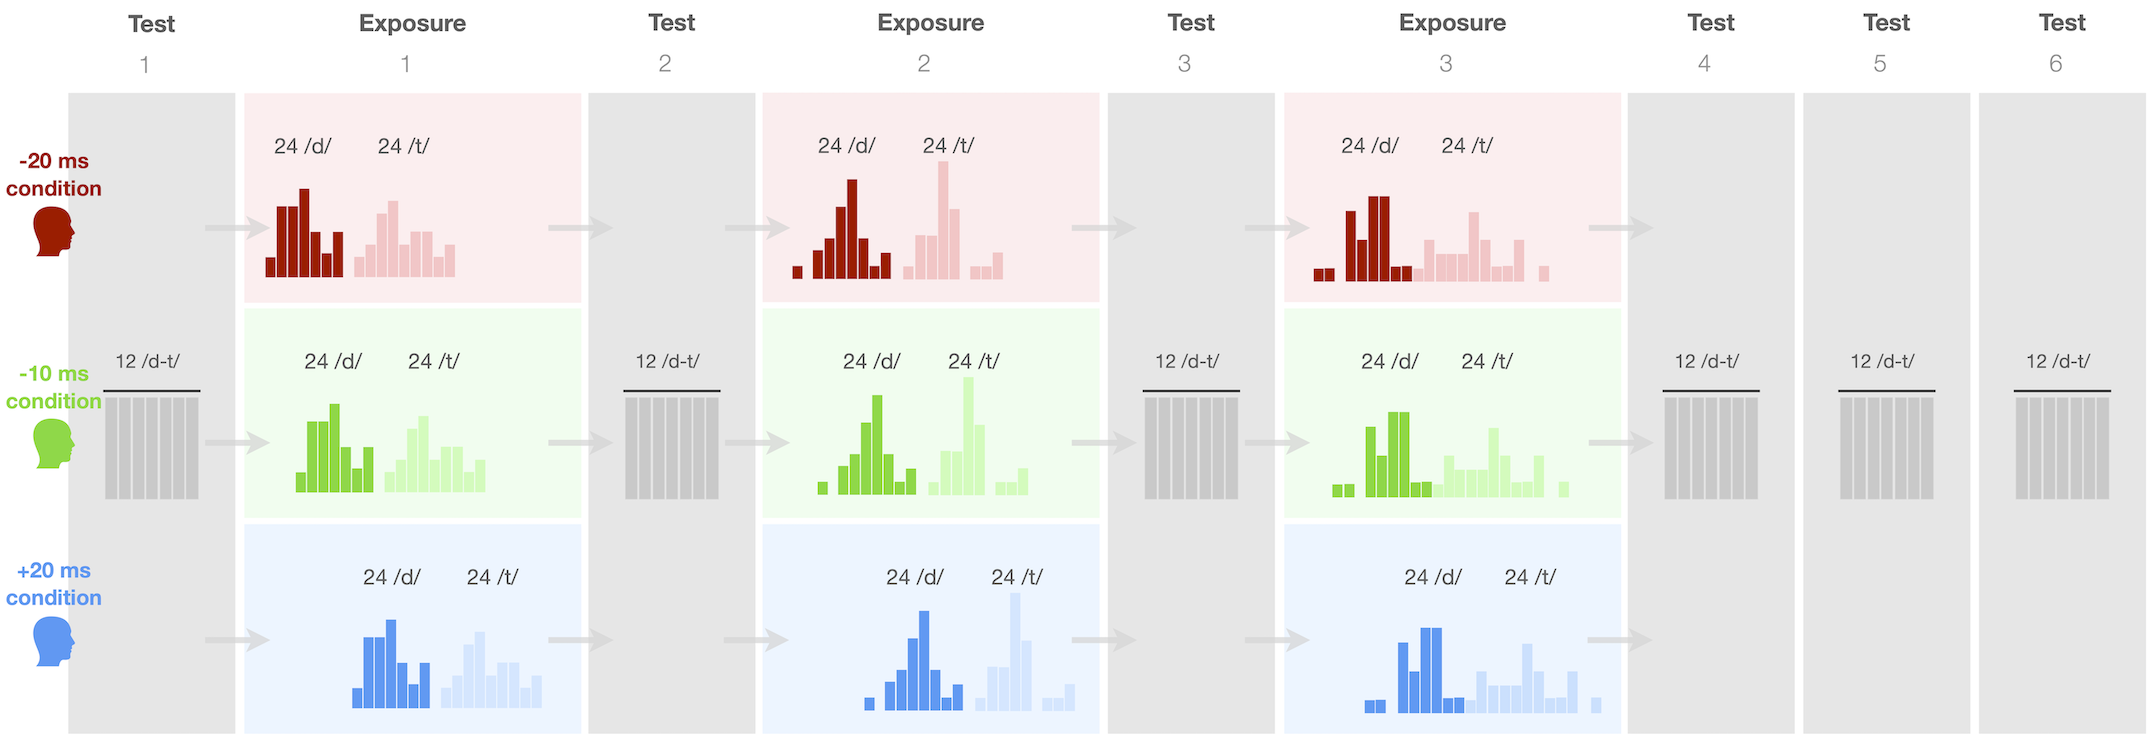
\includegraphics[width=5.8in]{../figures/block_design} 

}

\caption{Incremental exposure-test design of our experiment. The three exposure conditions (rows) differed in the distribution of voice onset time (VOT), the primary phonetic cue to syllable-initial /d/ and /t/ in English (e.g., "dip" vs. "tip"). Test blocks assessed L1-US English listeners' categorization functions over VOT stimuli that were held identical within and across conditions.}\label{fig:block-design-figure}
\end{figure}

Figure \ref{fig:block-design-figure} illustrates our approach. Between groups of participants, we manipulate the amount and distribution of phonetic cues in the exposure input. The three exposure distributions we use are shifted to different degrees both relative to each other, and relative to listeners' prior expectations. This allows us to test predictions (1) and (2a,b) that direction and magnitude of that change should gradiently depend on how and how much the current talker's speech deviates from the listeners' prior expectations. We measure listeners' categorization functions at multiple points during exposure, and determine whether the direction and magnitude of the observed changes in behavior are consistent with the predictions of distributional learning models, including prediction (4) about the diminishing rate of changes in listeners' behavior. To further guide the interpretation of results, we use normative models of adaptive speech perception \autocites[ideal observers and adaptors,][]{feldman2009,kleinschmidt-jaeger2015,massaro1989,xie2023}. This enables predictions about---intentionally idealized---listeners and distributional learners, prior to considerations about memory or other cognitive limitations. Comparisons of participants' categorization functions against these normative models provides a principled and informative approach to identifying constraints on adaptive speech perception, addressing prediction (3) about learning to convergence.

\begin{table}[!ht]
\begin{small}
\begin{tabular}{p{0.28\textwidth}p{0.7\textwidth}}
\hline
Prediction & Evidence that the {\em outcome} of learning is compatible with this prediction \\
\hline
(1) - {\em prior expectations} & (Kang \& Schertz, 2021; Schertz et al., 2016; Tan et al., 2021; Xie et al., 2021) \\

(2a) - {\em exposure amount}  & (Vroomen et al., 2007; Cummings \& Theodore, 2023; Kleinschmidt \& Jaeger, 2011; Liu \& Jaeger, 2018) \\

(2b) - {\em exposure distribution} & (Chl\'adkov\'a et al., 2017; Clayards et al., 2008; Colby et al., 2018; Hitczenko \& Feldman, 2016; Idemaru \& Holt, 2011; Kleinschmidt, 2020; Theodore \& Monto, 2019) \\

(3) - {\em learn to convergence}  & --- \\

(4) - {\em diminishing returns} & --- \\

\hline
\end{tabular}
\caption{Predictions of distributional learning models about incremental adaptation to an unfamiliar talker. To the best of our knowledge, only prediction (2a) has been tested against {\em incremental} changes in listeners' behavior, and predictions (3) and (4) have not been tested at all.}
\label{tab:predictions}
\end{small}
\end{table}

Our paradigm integrates, and builds on, advances in separate lines of research on unsupervised distributional learning during speech perception \autocite{clayards2008,colby2018,kleinschmidt2020,theodore-monto2019}, lexically- or visually-guided perceptual learning \autocite{cummings-theodore2023,kleinschmidt-jaeger2012,vroomen2007}, and adaptation to natural accents \autocite{hitczenko-feldman2016,tan2021,xie2021cognition}. We return to these and related works in the general discussion. For readers unfamiliar with this literature, we briefly make two observations that motivate the paradigm in Figure \ref{fig:block-design-figure}.

First, as indicated in Table \ref{tab:predictions}, previous research has focused on the \emph{outcome} of learning, leaving open whether adaptive speech perception unfolds over time in ways consistent with distributional learning models. For example, in an important early study, \textcite{clayards2008} exposed two different groups of US English listeners to instances of ``b'' and ``p'' that differed in their distribution along the voice onset time continuum (VOT). VOT is the primary phonetic cue to word-initial stops in US English: the voiced category (e.g., /b/, /d/, or /g/) is produced with lower VOT than the voiceless category (/p/, /t/, /k/). Clayards and colleagues held the VOT means of /b/ and /p/ constant between the two exposure groups, but manipulated whether both /b/ and /p/ had wide or narrow variance along VOT. Using a distributional learning model similar to the idealized learners we presented below, Clayards and colleagues predicted that listeners in the wide variance group would exhibit a more shallow categorization function than the narrow variance group. This is precisely what they found, providing support for prediction (2b) that the distribution of phonetic cues in the exposure input causes changes in listeners' behavior \autocites[see also][]{nixon2016,theodore-monto2019}. Findings like these suggests that the outcome of adaptation is qualitatively compatible with predictions (2a) and (2b) of distributional learning models \autocites[see also][]{hitczenko-feldman2016,tan2021,xie2021cognition}.\footnote{A related line of work has used distributional learning or explicit training paradigms to study the acquisition of \emph{novel} sound contrasts \autocites[e.g.,][]{maye2002,mcclelland1999,pajak-levy2012,pisoni1982}. These studies, too, have observed outcomes predicted by distributional learning models \autocite[for review, see][]{pajak2016}.}

These findings are, however, based on tests that averaged over, and/or followed, hundreds of exposure trials---exposure amounts that exceed what is available during many everyday interactions with unfamiliar talkers. This leaves open then whether the learning mechanism identified in distributional learning studies are sufficiently rapid to have a meaningful impact on those interactions. The strong focus on the outcome of adaptation also means that we do not know how listeners incrementally interpolate between their prior expectations and new phonetic input (the joint effects of predictions 1 and 2a,b). And it explains why predictions (3 - \emph{learn to convergence}) and (4 - \emph{diminishing returns}) have remained untested: tests of these two predictions require a repeated exposure-test paradigm like the one we present here \autocites[for discussion, see][]{cummings-theodore2023,kleinschmidt2020}.

Second, there often is a tension between ecological validity and the ability to make strong, quantitative predictions (though recent advances in automatic speech recognition and large language models might ultimately help resolve this tension). For these reasons, it has remained challenging to test distributional learning models against fully natural speech. This makes it difficult to test, on such stimuli, predictions (1) and (2b) about the effects of phonetic distributions listeners experience throughout their lifetime and during the experiment. Even recent tests against exposure to fully natural speech have thus focused on broad qualitative comparisons \autocites[e.g.,][]{schertz2016,xie2017}[see also,][]{schertz-clare2020}. This leaves open whether the direction and magnitude of changes in listeners' behavior can be explained by existing models \autocites[but see][]{hitczenko-feldman2016,tan2021,xie2021cognition}.

Tests of distributional learning models have thus largely relied on paradigms that afford researchers with fine-grained control over the distribution of phonetic properties that listeners experience in the experiment \autocites[e.g.,][]{chladkova2017,clayards2008,colby2018,idemaru-holt2011,kleinschmidt2020,theodore-monto2019}. As we aim to demonstrate below, such control is necessary for stronger tests of existing theories, but it often comes with sacrifices in ecological validity (for now, at least). We follow this approach here. As detailed under \emph{Methods}, we do, however, take several modest steps towards addressing concerns about ecological validity. This includes concerns about both the stimuli and their distribution in the experiment \autocite[see discussion in][]{baese-berk2018}.

To anticipate our results, we find that the changes in listeners' categorization behavior \emph{largely} follow the predictions of distributional learning models. In particular, we present the first direct evidence that the direction and magnitude of changes in listeners' categorization functions is jointly determined by their prior expectations (prediction 1) and the amount and distribution of phonetic cues in the exposure input (predictions 2a,b). We also find initial---though not decisive---evidence that changes in rate of adaptation throughout exposure are consistent with the predictions of error-driven learning theories and theories of ideal information integration (prediction 4). We show that a Bayesian model of adaptation that is based on principles of ideal information integration \autocites[the ideal adaptor,][]{kleinschmidt-jaeger2015,kleinschmidt-jaeger2016} predicts participants' responses with very high accuracy (\(R^2 = 97\%\)). However, not all observations we make are predicted by existing models, providing new insights into previously unrecognized limits of adaptation. In particular, we find little support for prediction (3 - \emph{learn to convergence}). Rather, changes in listeners' behavior seem to plateau long before listeners achieve the categorization functions and accuracy that would be expected if they fully learned the talkers' phonetic distributions (cf.~the \emph{premature convergence} panel of Figure \ref{fig:predictions}C). We also find that this constraint on adaptation seems to be asymmetric, depending on the direction of the shift in the exposure input relative to listeners' prior expectations. We discuss the implications of our findings for theories of adaptive speech perception, and suggest how future variants of our paradigm can be used to further contrast different models of adaptive speech perception.

\subsection{Open science}\label{open-science}

All data and code for this article are available on OSF at \url{https://osf.io/hxcy4/?view_only=270fc732415a49f5ab8f1fcaebf46b30}. The OSF repo also contains detailed supplementary information (SI) that we refer to throughout this article. Following \textcite{xie2023}, both this article and its SI are written in R Markdown. This allows other researchers to replicate and revise our analyses with the press of a button using freely available software \autocites[R,][]{R-base}[see also SI, \ref{sec:software}]{RStudio}.

This study was not publicly pre-registered. The design, participant recruitment, and procedure were internally pre-registered as part of an undergraduate class at the University of Rochester (BCS206/207). The experiment was originally designed to address predictions (1)-(3). Our analyses of prediction (4 - \emph{diminishing returns}) are thus post-hoc, as are some of the analyses we present to understand the evidence against prediction (3 - \emph{learn to convergence}). All post-hoc analyses are indicated as such. Finally, the ideal observer and adaptor models introduced below to guide interpretation of results follow our previous work \#\#\# \textbf{ommitted for review} \#\#\#. However, the choice of phonetic data on which these models are trained constitute researcher degrees of freedom. Where relevant, we motivate our decisions.

\section{Methods}\label{methods}

\subsection{Participants}\label{participants}

We recruited 126 participants from the Prolific crowdsourcing platform. Participants were randomly assigned to one of three exposure conditions in Figure \ref{fig:block-design-figure}. We used Prolific's pre-screening to limit the experiment to participants (1) of US nationality, (2) who reported to be English speaking monolinguals, and (3) had not previously participated in any experiment from our lab on Prolific. Prior to the start of the experiment, participants had to confirm that they (4) had spent the first 10 years of their life in the US, (5) were in a quiet place and free from distractions, and (6) wore in-ear or over-the-ears headphones that cost at least \$15.

Participants' responses were collected via Javascript developed by the Human Language Processing Lab at the University of Rochester \autocite{JSEXP2021} and stored via Proliferate developed at, and hosted by, the ALPs lab at Stanford University \autocite{Proliferate}. Participants took an average of 31.6 minutes (SD = 20 minutes) to complete the experiment and were remunerated \$8.00/hour. An optional post-experiment survey recorded participant demographics using NIH prescribed categories, including participant sex (female: 59, male: 60, declined to report: 3), age (mean = 38 years; SD = 12; 95\% quantiles = 20-62.1 years), ethnicity (Non-Hispanic: 113, Hispanic: 6, declined to report: 3), and race (due to a technical error, all information was lost).

\subsection{Materials}\label{materials}

We recorded 8 tokens each of four minimal word pairs with word-initial /d/-/t/ (\emph{dill/till}, \emph{dim/tim}, \emph{din/tin}, and \emph{dip/tip}) from a 23-year-old, female L1-US English talker from New Hampshire. In addition to these critical minimal pairs we also recorded three words that did not contain any stop consonant sounds (``flare'', ``share'', and ``rare''). These word recordings were used for catch trials. Stimulus intensity was normalized to 70 dB sound pressure level for all recordings.

The critical minimal pair recordings were used to create four VOT continua ranging from -100 to +130 ms in 5 ms steps.\footnote{We follow previous work \autocite{kleinschmidt2020,lisker-abramson1964} and refer to pre-voicing as negative VOTs though we note that pre-voicing is perhaps better conceived of as a separate phonetic feature \autocite[for discussion, see][]{mikuteit-reetz2007}. This distinction can, for example, be important when interpreting asymmetries in listeners' ability to adapt to left- vs.~rightward shifts along the VOT continuum, an issue we revisit in the general discussion.} Continua were generated using a script \autocite{winn2020} in Praat \autocite{boersma2022}. This approach resulted in continuum steps that sound natural, unlike the highly robotic-sounding stimuli employed in previous distributional learning studies \autocite[but see][]{theodore-monto2019}. It also maintained the natural correlations between the most important cues to word-initial stop-voicing in L1-US English (VOT, F0, and vowel duration). Specifically, the F0 at vowel onset of each stimulus was set to respect the linear relation with VOT observed in the original recordings of the talker. The duration of the vowel was set to follow the natural trade-off relation with VOT \autocite{allen-miller1999}. Further details on the recording and resynthesis procedure are provided in the SI (\ref{sec:stimulus-generation}). A post-experiment survey asked participants: ``\emph{Did you notice anything in particular about how the speaker pronounced the different words (e.g.~till, dill, etc.)?}'' No participant responded that the stimuli sounded unnatural. Analyses reported in the SI (\ref{sec:analysis-lapse}) found that participants exhibited few attentional lapses (\textless{} 1\%), including at the start of the experiment (\(\leq 1.5\)\%). This is a marked improvement over previous studies with robotic sounding stimuli, which elicited high lapse rates, especially at the start of the experiment \autocite[12\%,][]{kleinschmidt2020}. A norming experiment (N = 24 participants) was used to select the three minimal pair continua that differed the least from each other in terms of the categorization responses they elicited (\emph{dill-till}, \emph{din-tin}, and \emph{dip-tip}).

\subsection{Procedure}\label{sec:procedure}

At the start of the experiment, participants acknowledged that they met all requirements and provided consent, as per the Research Subjects Review Board of the University of Rochester. Participants had to pass a headphone test in order to continue \autocite{woods2017}, and were instructed to not change the volume throughout the experiment. Following instructions, participants completed 234 trials of two-alternative forced-choice categorization. Participants were given the opportunity to take breaks after every 60 trials, which was always during an exposure block. Finally, participants completed an exit survey and an optional demographics survey.

On each of the 234 categorization trials, participants heard a single word spoken by a female talker, and had to click on the word they heard (see Figure \ref{fig:example-trial}). Participants were instructed to ``answer as quickly and as accurately as possible''. Participants were also alerted to the fact that the recordings were subtly different and therefore may sound repetitive. Each trial started with a dark-shaded green fixation dot being displayed. At 500ms from trial onset, two minimal pair words appeared on the screen. At 1000ms from trial onset, the fixation dot would turn bright green and participants had to click on the dot to play the recording. This was meant to reduce trial-to-trial correlations by resetting the mouse pointer to the center of the screen at the start of each trial. Participants responded by clicking on the word they heard and the next trial would begin. Unbeknownst to participants, the 234 trials were split into three exposure blocks (54 trials each) and six test blocks (12 trials each), as shown in Figure \ref{fig:block-design-figure}.

\begin{figure}

{\centering 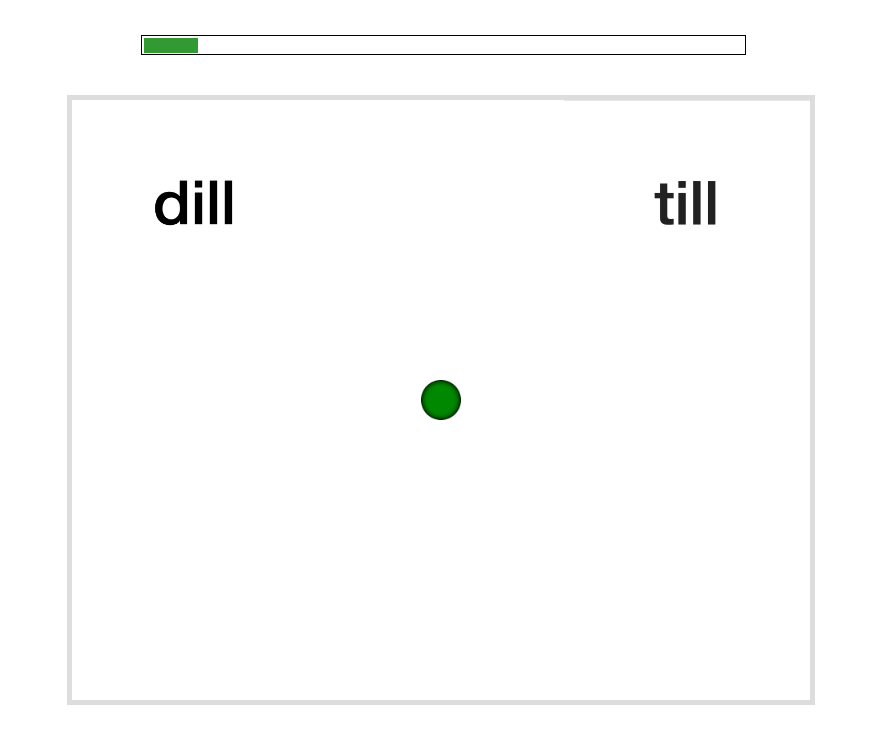
\includegraphics[width=0.33\linewidth]{../figures/trial_example} 

}

\caption{Example trial display. When the green button turned bright green, participants had to click on it to play the recording. The placement of response options was counter-balanced across participants.}\label{fig:example-trial}
\end{figure}

\emph{Test blocks. } The experiment started with a test block---often assumed, but not tested, to elicit identical response distributions across exposure conditions \autocites[see also][]{colby2018,xie2021cognition}. Test blocks were identical within and across conditions, always including 12 minimal pair trials assessing participants' categorization at 12 different VOTs (-5, 5, 15, 25, 30, 35, 40, 45, 50, 55, 65, 70 ms). The same brief test block followed each exposure block to assess the effects of cumulative exposure. As alluded to in the introduction, the use of repeated testing introduces procedural challenges.

Three considerations informed the decision to keep testing short. First, listeners' attention span is limited. Second, repeated testing over uniform test continua can reduce or undo the effects of informative exposure \autocite{cummings-theodore2023,zheng-samuel2023,liu-jaeger2018,liu-jaeger2019,giovannone-theodore2021,tzeng2021}. Third, the three exposure conditions differ in their exposure distributions, so that the ``same'' distribution in a test block will convey different information when evaluated relative to these exposure conditions. Theories of error-driven learning and ideal information integration (discussed in the introduction) predict that this affects adaptation. By keeping tests short relative to exposure, we aimed to minimize the influence of test trials on adaptation while still being able to estimate changes in listeners' categorization function.

The assignment of VOTs to minimal pair continua was randomized for each participant, but counter-balanced within and across test blocks. Each minimal pair appear equally often within each test block (four times), and each minimal pair appear with each VOT equally often (twice) across all six test blocks (and no more than once per test block). The order of response options---whether the /d/-initial word appeared on the left or right of the screen (see Figure \ref{fig:example-trial})---was held constant within each participant, and counter-balanced across participants.

\emph{Exposure blocks. } Each exposure block consisted of 24 /d/ and 24 /t/ trials, as well as 6 catch trials that served as a check on participant attention throughout the experiment (2 instances for each of three combinations of the three catch recordings). With a total of 144 trials, and intermittent tests after 0, 48, and 96 critical trials, the experiment was designed to measure the effects of exposure at substantially earlier moments than in similar previous experiments \autocites[cf.~\textgreater200 critical trials in][]{clayards2008,kleinschmidt2020,theodore-monto2019,nixon2016}.

The distribution of VOTs across the 48 /d/-/t/ trials depended on the exposure condition. We first created a \emph{baseline} condition. We set the VOT means to 5ms for /d/ and 50ms for /t/. We took two steps to increase the ecological validity of the VOT distributions, compared to similar previous work \autocite{clayards2008,idemaru-holt2011,idemaru-holt2020,kleinschmidt2015,kleinschmidt2020}. First, previous studies exposed each group of listeners to categories with identical variance. We instead set the variance for /d/ to 80 ms\(^2\) and for /t/ to 270 ms\(^2\) VOT. This qualitatively follows the natural asymmetry in the variance of VOT for /d/ and /t/ found in everyday speech \autocite{lisker-abramson1964,docherty1992,chodroff-wilson2017}.\footnote{The specific variance values we chose strike a compromise between the variance observed in natural productions \autocite[e.g, mean by-talker variances of 29 ms\(^2\) for /d/ and 275 ms\(^2\) for /t/ in hyper-articulated isolated word productions, and 70 ms\(^2\) for /d/ and 410 ms\(^2\) for /t/ in connected speech,][]{chodroff-wilson2017}, and the range of natural-sounding VOTs that we were able to generate with our procedure (for VOTs \textgreater{} 130ms, some recordings would not have sounded natural).} Second, rather than to expose listeners to fully symmetric \emph{designed} distributions that would never be experienced in everyday speech, we \emph{randomly sampled} from the intended VOT distribution (see top row of Figure \ref{fig:design-distribution}). Specifically, we sampled VOTs for three exposure blocks, and then created three Latin-square designed lists that counter-balanced the order of these blocks across participants.



\begin{figure}

{\centering \includegraphics{manuscript-main-file_files/figure-latex/design-distribution-1} 

}

\caption{Histogram of VOTs for each of the three exposure blocks A-C by exposure condition and trial type (labeled or unlabeled, sampled from /d/ or /t/). Each exposure block contained 12 labeled /d/, 12 labeled /t/, 12 unlabeled /d/, and 12 unlabeled /t/ trials, as well as 6 catch trials (not shown). Except for the shift in VOTs, the VOT distribution of these trials--as well as the relative placement of labeled and unlabeled trials---was identical across exposure conditions. The order of exposure blocks A-C was counter-balanced across participants within each exposure condition using a Latin-square design. Tick marks along the x-axis show the location of the twelve \emph{test} tokens, which were identical across conditions.}\label{fig:design-distribution}
\end{figure}

Following \textcite{kleinschmidt2015}, half of the /d/ and half of the /t/ trials in each exposure block were labeled, and the other half were unlabeled. Unlabeled trials were identical to test trials except that the distribution of VOTs across those trials was bimodal (rather than uniform), and determined by the exposure condition (see Figure \ref{fig:design-distribution}). Labeled trials instead presented two response options with identical stop onsets---e.g., \emph{din} and \emph{dill} to label the input as a /d/. While lexical context often disambiguates and labels sounds in everyday speech \autocites[facilitating adaptation,][]{burchill2023,burchill2018}, disambiguating context is not \emph{always} available. Especially with unfamiliar accents, listeners often have uncertainty about the word sequences they are hearing, reducing the labeling information available to them. Here, we thus struck a compromise between never or always labeling the input.

Next, we created the two additional exposure conditions by shifting all VOTs sampled for the baseline condition by +10 or +40 ms (see Figure \ref{fig:design-distribution}). This approach exposes participants to heterogeneous \emph{samples} of VOT distributions for /d/ and /t/ that varied across blocks, while holding all aspects of the input constant across conditions except for the shift in VOT---including the placement of labeled and unlabeled trials relative to the exposure condition's category means. The order of trials was randomized within each block and participant, with no more than two catch trials in a row. Participants were randomly assigned to one of 18 lists, crossing 3 (exposure condition) x 3 (block order) x 2 (placement of response options during unlabeled test and exposure trials). We note that the naming of conditions (baseline, +10, +40) should be understood as \emph{relative to each other}, rather than relative to listeners' prior experience.

\subsection{Exclusions}\label{exclusions}

Exclusion criteria were determined prior to analysis. Due to data transfer errors, four participants' data were not stored and therefore excluded from analysis. We further excluded from analysis participants who committed more than three errors out of the 18 catch trials (\textless83\% accuracy, N = 1), participants who committed more than four errors out of the 72 labelled trials (\textless94\% accuracy, N = 0), participants with an average reaction time more than three standard deviations from the mean of the by-participant means (N = 0), participants who had atypical categorization functions even prior to exposure (N = 2, see SI, \ref{sec:exclusions} for details), and participants who reported not to have used headphones (N = 0). This left for analysis 17,136 exposure and 8,568 test observations from 119 participants (94\% of total), approximately evenly split across the three exposure conditions (baseline: 40 participants; +10: 40; +40: 39).

\section{Results}\label{sec:results}

Below, we begin by describing our analysis approach, which deviates from previous work. We therefore first demonstrate that our approach replicates previous findings when applied to our data at the level of analysis employed in previous work: the detection of overall changes in listeners' categorization behavior after exposure. Following this, we turn to our primary questions: \emph{incremental} changes in participants' categorization responses from pre-exposure onward, depending on the type (exposure condition) and amount of exposure (test block). This allow us to assess predictions (1) and (2a,b) about the role of prior and recent experience in explaining incremental adaptive speech perception, as well as prediction (4) about the diminishing rate of behavioral changes with increasing exposure. To facilitate the interpretation of our results, we introduce normative models (ideal observers) that determine the expected categorization functions of idealized listeners prior to, and following, exposure (following the same approach used in Figure \ref{fig:predictions}). This allows us to identify previously unrecognized constraints on adaptive speech perception (prediction 3 - learning to convergence).

\subsection{Analysis approach}\label{analysis-approach}

We analyzed participants' categorization responses during exposure and test blocks in two separate Bayesian mixed-effects psychometric models, using \texttt{brms} \autocite{R-brms_a} in \texttt{R} \autocite{R,RStudio}.\footnote{For the analyses of test blocks, fitting the models separately removes any potential collinearity between effects of exposure and effects of VOT. The SI reports additional analyses over the combined data, including extensions of the psychometric models to include lapse rates that can vary by block (\ref{sec:analysis-lapse}) and non-parametric smooths to model non-linear effects of VOT and exposure (\ref{sec:GAMM}). All analyses replicate the findings reported here.} Psychometric models account for attentional lapses while estimating participants' categorization functions. Failing to account for attentional lapses---while still common in research on speech perception \autocites[for exceptions, see][]{clayards2008,kleinschmidt-jaeger2016}---can lead to biased estimates of categorization boundaries \autocite{prins2011,wichmann-hill2001}. For the advantages of Bayesian psychometric models, we refer to \textcite{kuss2005} and \textcite{prins2019}. For the present experiment, lapse rates were negligible (0.8\%, 95\%-CI: 0.4 to 1.5\%), and all results replicate in simple mixed-effects logistic regressions \autocite{jaeger2008}. These lapse rates compare favorably against those assumed or reported in prior work \autocites[e.g.,][]{clayards2008,kleinschmidt-jaeger2016,kleinschmidt2020}.

The psychometric models for exposure and test blocks each regressed participants' categorization responses against the full factorial interaction of VOT, block, and exposure condition, along with the maximal random effect structure (by-participant intercepts and slopes for VOT, block, and their interaction, and by-item intercept and slopes for the full factorial design; see SI, \ref{sec:analysis-approach}). All hypothesis tests reported below are based on these models. Figure \ref{fig:plot-fit-PSE} summarizes the results that we describe in more detail next. Panels A and B show participants' categorization responses during exposure and test blocks, along with the categorization function estimated from those responses via the mixed-effects psychometric models. These panels facilitate comparison between exposure conditions within each block. Panel C summarizes changes in listeners' point of subject equality (PSE)---i.e., the point along the VOT continuum at which participants are equally likely to respond ``d'' or ``t''---across blocks and conditions. This highlights how the type and amount of phonetic input affect listeners' categorization functions. Here we focus on the test blocks, which were identical within and across exposure conditions. Analyses of the exposure blocks, reported in the SI (\ref{sec:SI-exposure-block-analysis}), replicate all effects found in the test blocks.

\subsection{Conceptual replication (averaging over test blocks)}\label{conceptual-replication-averaging-over-test-blocks}

We first use the psychometric mixed-effects model to analyze participants' behavior averaged over all test blocks. This analysis recasts, within a psychometric model, the type of analysis most common in the field: it assesses overall changes in listeners' behavior after exposure, without telling us how these changes accumulate, how they relate to listeners' prior expectations, or how they compare to behavior that would be expected from a learner that has fully adapted to the unfamiliar talker. Prediction (2b) states that changes in listeners' categorization function should depend on the distribution of phonetic cues in the exposure input. Specifically, the +10 condition should elicit a rightward shift in the categorization function relative to the baseline condition, and the +40 condition should elicit an even larger rightward shift. This is also what previous work found \autocite{kleinschmidt-jaeger2016}.

Across all test blocks, participants were more likely to respond ``t'' the longer the VOT (\(\hat{\beta} = 15.09\), 90\%-CI = \([12.377, 17.625]\), \(BF \geq 8000\), \(p_{posterior} =\) \(1\)). Exposure affected participants' categorization responses in the predicted direction. Marginalizing over Tests 1-6, participants in the +40 condition were less likely to respond ``t'' than participants in the +10 condition (\(\hat{\beta} = -2.26\), 90\%-CI = \([-3.258, -1.228]\), \(BF = 162.27\), \(p_{posterior} =\) \(0.994\)) or the baseline condition (\(\hat{\beta} = -3.08\), 90\%-CI = \([-4.403, -1.669]\), \(BF = 215.22\), \(p_{posterior} =\) \(0.995\)). There was also evidence---albeit less decisive---that participants in the +10 condition were less likely to respond ``t'' than participants in the baseline condition (\(\hat{\beta} = -0.82\), 90\%-CI = \([-1.887, 0.282]\), \(BF = 8.91\), \(p_{posterior} =\) \(0.899\)). That is, the +10 and +40 conditions resulted in categorization functions that were shifted rightwards compared to the baseline condition, as also evident in Figure \ref{fig:plot-fit-PSE}A.\footnote{The perceptual model contained in the our psychometric mixed-effects model describes the effect of VOT on the log-odds of ``t''-responses as a line. The main effect of VOT is the average slope of that line across exposure conditions. The \(\hat{\beta}\)s for the comparisons across conditions indicate differences in the intercept of that line. Negative \(\hat{\beta}\)s thus indicate a \emph{down}ward shift of that line in one condition, relative to the other. These downward shifts result in \emph{right}ward shifts of the point of subjective equality (PSE), the VOT at which ``t'' and ``d'' responses are equally likely. This also shows in Figure \ref{fig:plot-fit-PSE}A. In this figure, predictions are transformed into proportion ``t''-responses and the downward shifts appear visually as a rightward shifts of the S-shaped categorization function (of one condition relative to another).}

Unlike the differences in the relative shift of the categorization function, there was little evidence that the \emph{slopes} of listeners' categorization functions differed between exposure conditions (0.73 \textless{} BFs \textless{} 2.1; see also Figure \ref{fig:plot-fit-PSE}A). This lack of notable differences in the slope is precisely what is expected under distributional learning models, since our exposure conditions manipulated neither the category variances of /d/ and /t/ nor the distance between their category means. In the remainder of the main text, we thus focus on right vs.~left shifts in listeners' categorization function---i.e., changes in listeners' PSE. Parallel analyses of changes (or lack thereof) in the slopes of listeners' categorization functions are reported in the SI (\ref{sec:slopes-analyses-test}-\ref{sec:slopes-analyses-exposure}), and do not affect any of our conclusions.

In summary, our initial analysis conceptually replicates previous findings that exposure to different VOT distributions changes listeners' categorization responses \autocites[for /b/-/p/:][]{clayards2008,kleinschmidt2015,kleinschmidt2020}[for /g/-/k/,][]{theodore-monto2019}. This replication makes two noteworthy contributions. It extends previous findings to stimuli and stimulus distributions that somewhat more closely resemble those found in everyday speech. And it adds to a small body of work that goes beyond dichotomous comparisons, testing stronger hypotheses about the relative ordering of multiple exposure conditions \autocites[e.g.,][]{babel2019,bejjanki2011,bradlow-bent2008,cummings-theodore2023,kleinschmidt2020,liu-jaeger2018}.

\subsection{Overview of incremental analyses}\label{overview-of-incremental-analyses}

Next, we turn to our primary questions. We assess incremental changes in participants' categorization responses from three mutually complementing perspectives (all based on the same psychometric mixed-effects model). First, we compare the effects of different exposure conditions within each block. This is the perspective taken in previous studies and in the conceptual replication presented above, but extended to test \emph{how early} in the experiment differences between exposure conditions begin to emerge. Second, we compare \emph{within} each condition how exposure \emph{incrementally changes} listeners' categorization responses from block to block within each condition, relative to listeners' responses prior to any exposure. Together with the first perspective, this allows us to test predictions (1 - \emph{prior expectations})-(2a,b - \emph{exposure amount \& distribution}). Third, we compare changes in listeners' responses to those expected from an ideal observer that has fully learned the exposure distributions. This analysis has the potential to identify constraints on cumulative adaptation. As we show, the latter two perspectives---made possible by the incremental exposure-test paradigm---afford stronger tests of predictions (3 - \emph{learn to convergence}) and (4 - \emph{diminishing returns}), and suggest previously unrecognized constraints on the early moments of adaptive speech perception. For all three analyses, we initially focus on Tests 1-4 with intermittent exposure. Finally, we analyze the effects of repeated testing without intermittent exposure blocks during Tests 4-6. This reveals that such testing has under-appreciated methodological and theoretical consequences.



\begin{landscape}







\begin{figure}

{\centering \includegraphics{manuscript-main-file_files/figure-latex/plot-fit-PSE-1} 

}

\caption{Summary of results. \textbf{Panel A:} Changes in listeners psychometric categorization functions as a function of exposure, from Test 1 to Test 4 with all intervening exposure blocks (only unlabeled trials were included in the analysis of exposure blocks since labeled trials provide little information about listeners' categorization function). Point ranges indicate the mean proportion of participants' ``t''-responses and their 95\% bootstrapped CIs. Lines and shaded intervals show the \emph{maximum a posteriori} (MAP) estimates and 95\%-CIs of a Bayesian mixed-effects psychometric model fit to participants' responses. \textbf{Panel B:} Same as Panel A but for the final three test blocks without intervening exposure. Test 4 is shown as part of both Panels A and B. \textbf{Panel C:} Changes across blocks and conditions in listeners' point-of-subjective-equality (PSE) of the lapse-corrected categorization functions from Panels A \& B (i.e., the PSE of the perceptual model inferred from listeners' responses; for changes in the slope of that function, see SI, \ref{sec:io-bias-correction}). Point ranges represent the posterior medians and their 95\%-CIs derived from the psychometric model. Horizontal dashed lines indicate 95\%-CIs of the PSEs expected from an idealized learner (an ideal observer model that has fully learned the exposure distributions). Percentage labels indicate the degree of shift in PSE exhibited by participants as a proportion of the expected shift under the idealized learners (for details, see SI, \ref{sec:shrinkage-test-all}). Horizontal gray ribbon indicates the 95\%-CIs of the PSEs expected from an idealized listener \emph{prior to any exposure}.}\label{fig:plot-fit-PSE}
\end{figure}

\end{landscape}

\subsection{How early does exposure begin to affect listeners' categorization responses? (comparing exposure conditions within each test block)}\label{how-early-does-exposure-begin-to-affect-listeners-categorization-responses-comparing-exposure-conditions-within-each-test-block}

\begin{table}[H]
\centering
\caption{\label{tab:hypothesis-table-simple-effects-condition}The simple effects of the exposure conditions for each test block. This analysis asks how early exposure starts to affect participants’ categorization responses, and when (if ever) these changes were undone with repeated testing. Note that rightward shifts of the categorization function (and its PSE) correspond to negative estimates (lower intercepts in predicting the log-odds of ``t''-responses). Predicted nulls for Test 1 were tested using the Savage-Dickey density ratio.}
\centering
\begin{tabular}[t]{>{\raggedright\arraybackslash}p{15em}rrrrr}
\toprule
Hypothesis & Est. & SE & 90\%-CI & BF & $p_{post}$\\
\midrule
\addlinespace[0.3em]
\multicolumn{6}{l}{\textbf{Test block 1 (pre-exposure)}}\\
\hspace{1em}$PSE_{+10} = PSE_{baseline}$ & -0.34 & 0.75 & {}[-2.03, 1.44] & 3.3 & 0.77\\
\hspace{1em}$PSE_{+40} = PSE_{+10}$ & 0.25 & 0.73 & {}[-1.34, 1.9] & 3.7 & 0.79\\
\hspace{1em}$PSE_{+40} = PSE_{baseline}$ & -0.08 & 0.91 & {}[-2.12, 2.08] & 4.8 & 0.83\\
\addlinespace[0.3em]
\multicolumn{6}{l}{\textbf{Test block 2}}\\
\hspace{1em}$PSE_{+10} > PSE_{baseline}$ & -1.45 & 0.89 & {}[-2.93, 0.18] & 13.7 & 0.93\\
\hspace{1em}$PSE_{+40}  > PSE_{+10}$ & -2.08 & 0.99 & {}[-3.82, -0.17] & 24.3 & 0.96\\
\hspace{1em}$PSE_{+40} > PSE_{baseline}$ & -3.49 & 1.24 & {}[-5.63, -1.07] & 54.2 & 0.98\\
\addlinespace[0.3em]
\multicolumn{6}{l}{\textbf{Test block 3}}\\
\hspace{1em}$PSE_{+10} > PSE_{baseline}$ & -0.78 & 0.62 & {}[-1.89, 0.36] & 7.9 & 0.89\\
\hspace{1em}$PSE_{+40}  > PSE_{+10}$ & -2.80 & 0.82 & {}[-4.19, -1.11] & 86.0 & 0.99\\
\hspace{1em}$PSE_{+40} > PSE_{baseline}$ & -3.56 & 0.97 & {}[-5.2, -1.58] & 110.1 & 0.99\\
\addlinespace[0.3em]
\multicolumn{6}{l}{\textbf{Test block 4}}\\
\hspace{1em}$PSE_{+10} > PSE_{baseline}$ & -0.88 & 0.85 & {}[-2.36, 0.85] & 4.8 & 0.83\\
\hspace{1em}$PSE_{+40}  > PSE_{+10}$ & -3.32 & 0.89 & {}[-4.88, -1.64] & 128.0 & 0.99\\
\hspace{1em}$PSE_{+40} > PSE_{baseline}$ & -4.16 & 1.21 & {}[-6.28, -1.88] & 122.1 & 0.99\\
\addlinespace[0.3em]
\multicolumn{6}{l}{\textbf{Test block 5 (repeated testing without additional exposure)}}\\
\hspace{1em}$PSE_{+10} > PSE_{baseline}$ & -1.33 & 0.71 & {}[-2.56, 0] & 19.2 & 0.95\\
\hspace{1em}$PSE_{+40}  > PSE_{+10}$ & -2.39 & 0.86 & {}[-3.89, -0.8] & 65.1 & 0.98\\
\hspace{1em}$PSE_{+40} > PSE_{baseline}$ & -3.72 & 1.01 & {}[-5.5, -1.7] & 139.4 & 0.99\\
\addlinespace[0.3em]
\multicolumn{6}{l}{\textbf{Test block 6 (repeated testing without additional exposure)}}\\
\hspace{1em}$PSE_{+10} > PSE_{baseline}$ & -0.22 & 0.72 & {}[-1.48, 1.11] & 1.7 & 0.62\\
\hspace{1em}$PSE_{+40}  > PSE_{+10}$ & -1.70 & 0.79 & {}[-3.08, -0.17] & 25.0 & 0.96\\
\hspace{1em}$PSE_{+40} > PSE_{baseline}$ & -1.91 & 0.99 & {}[-3.63, 0.02] & 18.5 & 0.95\\
\bottomrule
\end{tabular}
\end{table}

Figure \ref{fig:plot-fit-PSE}A suggests that differences between exposure conditions emerged very early in the experiment. This is confirmed by Bayesian hypothesis tests summarized in Table \ref{tab:hypothesis-table-simple-effects-condition}, which we discuss next. Prior to any exposure, during Test 1, participants' responses did not differ across exposure conditions. This result is predicted by models of adaptive speech perception under the assumptions that (a) participants in the different groups have similar prior experiences, and that (b) our sample size is sufficiently large to yield stable estimates of listeners' categorization function.\footnote{ The moderate BFs for these hypothesis tests are due to our use of regularizing priors, which have non-negligible density over the null \autocite[for an introduction to the Savage-Dickey method, see][]{wagenmakers2010}. Rather than to test the null against more plausible alternative priors, which would predictably increase the evidence for the null, we appeal to readers' intuition: the 90\%-CIs of the comparisons for Test 1 are all approximately centered around zero; there is very little evidence in favor of an effect in either direction.} Equality of pre-exposure behavior across exposure groups is also implicitly assumed---but rarely tested---in the interpretation of most studies on adaptive speech perception \autocite[when it is tested, it often turns out that this assumption is \emph{not} necessarily warranted, presumably due to insufficient sample sizes, cf.][]{kleinschmidt2020}.

During Test 2, after exposure to only 24 /d/ and 24 /t/ stimuli (thereof half labeled), participants' categorization responses already differed between exposure conditions (BFs \textgreater{} 14). All differences between exposure conditions that emerged at Test 2 followed prediction (2b - \emph{exposure distributions}). Additional analyses reported in the SI (\ref{sec:SI-exposure-block-analysis}) found that listeners' categorization functions had already changed in the predicted direction during the first \emph{exposure} block, in line with Figure \ref{fig:plot-fit-PSE}A. This suggests that changes in listeners' categorization responses emerged quickly at the earliest point tested---after only a fraction of exposure trials previously tested in similar paradigms.

The effects of the three exposure conditions persisted until Test 4, always in line with prediction (2b). Table \ref{tab:hypothesis-table-simple-effects-condition} does, however, indicate an interesting non-monotonic development. While the difference between the +40 condition and both the baseline and +10 condition continued to increase numerically with increasing exposure (increasingly larger magnitude of negative estimates in Tests 2-4), the same was not the case for the difference between the +10 and the baseline condition. Instead, the difference between the +10 and baseline condition \emph{reduced} with increasing exposure (while maintaining its direction; from \(\hat{\beta} =\) -1.4 to \(\hat{\beta} =\) -0.83, see Table \ref{tab:hypothesis-table-simple-effects-condition}). At first blush, this non-monotonicity appears to contradict prediction (2a) that the magnitude of exposure effects should increase with increasing exposure. In the next section, we show that the results do, in fact, \emph{support} prediction (2a) when listeners' prior expectations are considered. Indeed, the seemingly unexpected non-monotonicity---which would be impossible to detect without repeated testing---turns out to be important for understanding incremental adaptation.

\subsection{Incremental adaptation from prior expectations (comparing block-to-block changes within exposure conditions)}\label{incremental-adaptation-from-prior-expectations-comparing-block-to-block-changes-within-exposure-conditions}

Next, we compare how listeners' categorization responses changed from block to block \emph{within} each exposure condition. This allows us to understand changes in listeners' categorization function relative to listeners' pre-exposure behavior, thereby assessing the joint effects of predictions (1 - \emph{prior expectations}) and (2a,b - \emph{exposure amount \& distributions}). To facilitate visual comparison across blocks and conditions, Figure \ref{fig:plot-fit-PSE}C summarizes the block-to-block changes in listeners' PSE. Focusing for now on Tests 1-4, this highlights three aspects of participants' behavior that were not readily apparent in the statistical comparisons presented so far.

\begin{table}[H]
\centering
\caption{\label{tab:hypothesis-table-simple-effects-block}Was there incremental change from test block 1 to 4? Did these changes dissipate with repeated testing from block 4 to 6? This table summarizes the simple effects of block for each exposure condition. Note that rightward shifts of the categorization function (and its PSE) correspond to negative estimates (lower intercepts in predicting the log-odds of ``t''-responses).}
\centering
\begin{tabular}[t]{>{\raggedright\arraybackslash}p{15em}rrrrr}
\toprule
Hypothesis & Est. & SE & 90\%-CI & BF & $p_{post}$\\
\midrule
\addlinespace[0.3em]
\multicolumn{6}{l}{\textbf{Difference between blocks: baseline}}\\
\hspace{1em}Block 1 to 2: decreased PSE & 1.16 & 0.71 & {}[-0.22, 2.52] & 12.9 & 0.93\\
\hspace{1em}Block 2 to 3: decreased PSE & 0.12 & 0.70 & {}[-1.31, 1.48] & 1.3 & 0.57\\
\hspace{1em}Block 3 to 4: decreased PSE & 0.17 & 0.53 & {}[-0.86, 1.12] & 1.7 & 0.63\\
\hspace{1em}{\em Block 1 to 4: decreased PSE} & 1.48 & 1.13 & {}[-0.73, 3.44] & 7.6 & 0.88\\
\hspace{1em}Block 4 to 5: increased PSE & -0.37 & 0.49 & {}[-1.28, 0.53] & 3.5 & 0.78\\
\hspace{1em}Block 5 to 6: increased PSE & -0.57 & 0.61 & {}[-1.65, 0.62] & 4.6 & 0.82\\
\hspace{1em}{\em Block 4 to 6: increased PSE} & -0.94 & 0.73 & {}[-2.29, 0.51] & 7.2 & 0.88\\
\addlinespace[0.3em]
\multicolumn{6}{l}{\textbf{Difference between blocks: +10}}\\
\hspace{1em}Block 1 to 2: decreased PSE & 0.16 & 0.79 & {}[-1.17, 1.62] & 1.4 & 0.59\\
\hspace{1em}Block 2 to 3: decreased PSE & 0.60 & 0.66 & {}[-0.57, 1.85] & 4.5 & 0.82\\
\hspace{1em}Block 3 to 4: decreased PSE & 0.17 & 0.77 & {}[-1.32, 1.64] & 1.4 & 0.58\\
\hspace{1em}{\em Block 1 to 4: decreased PSE} & 0.94 & 1.21 & {}[-1.3, 3.17] & 3.5 & 0.78\\
\hspace{1em}Block 4 to 5: increased PSE & -0.58 & 0.58 & {}[-1.63, 0.52] & 4.9 & 0.83\\
\hspace{1em}Block 5 to 6: increased PSE & 0.44 & 0.65 & {}[-0.79, 1.65] & 0.3 & 0.24\\
\hspace{1em}{\em Block 4 to 6: increased PSE} & -0.12 & 0.83 & {}[-1.63, 1.48] & 1.3 & 0.56\\
\addlinespace[0.3em]
\multicolumn{6}{l}{\textbf{Difference between blocks: +40}}\\
\hspace{1em}Block 1 to 2: increased PSE & -2.06 & 0.79 & {}[-3.43, -0.56] & 45.2 & 0.98\\
\hspace{1em}Block 2 to 3: increased PSE & -0.73 & 0.78 & {}[-2.09, 0.63] & 4.7 & 0.83\\
\hspace{1em}Block 3 to 4: increased PSE & -0.06 & 0.81 & {}[-1.48, 1.34] & 1.1 & 0.53\\
\hspace{1em}{\em Block 1 to 4: increased PSE} & -2.86 & 1.12 & {}[-4.87, -0.73] & 50.3 & 0.98\\
\hspace{1em}Block 4 to 5: decreased PSE & 0.61 & 0.77 & {}[-0.75, 1.93] & 3.6 & 0.78\\
\hspace{1em}Block 5 to 6: decreased PSE & 0.75 & 0.72 & {}[-0.56, 2] & 5.5 & 0.85\\
\hspace{1em}{\em Block 4 to 6: decreased PSE} & 1.36 & 0.95 & {}[-0.33, 2.99] & 10.3 & 0.91\\
\bottomrule
\end{tabular}
\end{table}

First, while the PSEs for the +40 and +10 conditions were shifted rightwards compared to the baseline condition, both the +10 and the baseline condition seem to shift \emph{left}wards relative to their pre-exposure starting point in Test 1. Bayesian hypothesis tests summarized in Table \ref{tab:hypothesis-table-simple-effects-block} find moderate support for a leftward shift from Test 1 to 4 in both the +10 condition (BF = 3.5) and the baseline condition (BF = 7.6). In contrast, there was strong support that the +40 condition shifted rightwards relative to pre-exposure (BF = 50).

To understand this pattern, it is helpful to relate the three exposure conditions to the phonetic distribution in listeners' prior experience. Figure \ref{fig:exposure-means-database-matrix-plot} shows the exposure means for /d/ and /t/ relative to the distributions of three important cues to the word-initial /d/-/t/ contrast in L1-US English. For this purpose, we chose a database of word-initial /d/s and /t/s from isolated word productions \autocite{chodroff-wilson2018}. Compared to databases of connected speech, these isolated recordings more closely approximate the speech rate of our stimuli \autocites[which is known to affect the perception of VOT,][]{allen-miller1999,utman1998}. The SI \ref{sec:placement-of-exposure-stimuli} provides the same visualization, while also showing the distributions for 1,052 words produced in connected speech by 13 female talkers from the same database (confirming the conclusions reached here).

Figure \ref{fig:exposure-means-database-matrix-plot} offers an explanation as to why the baseline condition (and to some extent the +10 condition) shift leftwards with increasing exposure, whereas the +40 condition shifts rightwards: relative to the distribution of VOT for /d/ and /t/ in listeners' prior experience, only the +40 condition presents category means that are clearly larger than expected along VOT, whereas the baseline condition and, to some extent, the +10 condition presented lower-than-expected category means. That is, once we take into account how our exposure conditions relate to listeners' prior experience (prediction 1), both the direction of changes from Test 1 to 4 \emph{within} each exposure condition (Table \ref{tab:hypothesis-table-simple-effects-block}), and the direction of differences \emph{between} exposure conditions receive an explanation (Table \ref{tab:hypothesis-table-simple-effects-condition}). To further illustrate this point, the horizontal gray ribbon in \ref{fig:plot-fit-PSE}C shows the range of PSEs predicted by Bayesian ideal observers trained on the distribution of VOT, f0, and vowel duration for isolated word productions in Figure \ref{fig:exposure-means-database-matrix-plot} (for details, see SI, \ref{sec:idealized-prior-listeners}).



\begin{figure}[!ht]

{\centering \includegraphics{manuscript-main-file_files/figure-latex/exposure-means-database-matrix-plot-1} 

}

\caption{Placement of exposure conditions (category means of /d/ and /t/, shown in color) relative to an estimate of L1 US English listeners' prior expectations. After VOT, f0 and vowel duration are two of the most informative cues to word-initial /d/-/t/ in L1 US English. As an estimate of listeners' prior expectations about these distributions, we show 1,052 word-initial /d/ and /t/ productions for words produced in isolation by 13 female L1 talkers in \textcite{chodroff-wilson2018}. The upper off-diagonal shows each of these productions as a point. The diagonal shows their marginal density, with a data rug at the bottom indicating the placement of exposure means. The lower off-diagonal shows bivariate Gaussians fit to the distribution of the /d/ and /t/ productions, with the exposure means for each condition indicated by the /d/ and /t/ labels.}\label{fig:exposure-means-database-matrix-plot}
\end{figure}

Second, we find support for prediction (4) about the \emph{diminishing returns} of additional exposure predicted by some theories of adaptive speech perception. The estimates in Table \ref{tab:hypothesis-table-simple-effects-block} suggest that listeners' PSEs changed most substantially from Test 1 to Test 2, and then changed less and less with additional exposure up to Test 4 (smaller magnitude of estimates compared to earlier test blocks). This seems to be particularly pronounced for the baseline condition and the +40 condition---the two conditions that exhibited the largest shifts relative to pre-exposure. As mentioned in our Open Science statement, our experiment was not designed to have high power to assess such \emph{changes in the magnitude of the shifts} across the block within each condition. We did, however, conduct post-hoc hypothesis tests to assess the support for this pattern. These tests found anecdotal to moderately strong evidence in support of prediction (4 - \emph{diminishing returns}). For the +40 condition, the shift from Test 1 to 2 was larger than the shift from Test 2 to 3 (\(\hat{\beta} = -1.31\), 90\%-CI = \([-3.518, 0.904]\), \(BF = 5.44\), \(p_{posterior} =\) \(0.845\)), which was larger than the shift from Test 3 to 4 (\(\hat{\beta} = -0.67\), 90\%-CI = \([-2.861, 1.546]\), \(BF = 2.35\), \(p_{posterior} =\) \(0.702\)). Comparing the change from Test 1 to 2 against the change from Test 3 to 4, there was stronger support that the speed of changes in the PSE decreased (\(\hat{\beta} = -1.98\), 90\%-CI = \([-4.067, 0.2]\), \(BF = 14.9\), \(p_{posterior} =\) \(0.937\)). For the baseline condition, the shift from Test 1 to 2 was larger than the shift from Test 2 to 3 (\(\hat{\beta} = 1.05\), 90\%-CI = \([-1.046, 3.142]\), \(BF = 4.37\), \(p_{posterior} =\) \(0.814\)), which was almost identical, but slightly smaller, than the shift from Test 3 to 4 (\(\hat{\beta} = 0.04\), 90\%-CI = \([-1.805, 1.86]\), \(BF = 1.06\), \(p_{posterior} =\) \(0.515\)). Again, a comparison of the change from Test 1 to 2 against the change from Test 3 to 4, yielded the strongest support that the speed of changes in the PSE decreased (\(\hat{\beta} = 1.01\), 90\%-CI = \([-0.745, 2.821]\), \(BF = 5.34\), \(p_{posterior} =\) \(0.842\)). For both the +40 and the baseline condition, there was only anecdotal evidence that the final exposure block resulted in \emph{any additional} shift in listeners' PSE (BFs \(\leq\) 1.7, cf.~Table \ref{tab:hypothesis-table-simple-effects-block}).

Third and finally, Panel C also begins to illuminate the reasons for the non-monotonic development of the +10 and baseline conditions relative to each other, discussed in the previous section. In particular, this non-monotonicity does \emph{not} appear due to a reversal of the effects in either of the two exposure conditions. Rather, both exposure conditions continue to change listeners' categorization function in the same direction from Test 1 to Test 4, in line with predictions (2a) and (2b). However, after the rapid change from the pre-exposure Test 1 to the first post-exposure Test 2, listeners' categorization responses in the baseline condition did not change as much as in the +10 condition. In fact, listeners' categorization function in the baseline condition seems to have plateaued after the first exposure block.

This explains the reduction in the difference between the +10 and baseline conditions discussed in the previous section. It does, however, raise the question \emph{why} listeners' responses in the baseline condition did not change further with increasing exposure. One explanation would be that participants in the baseline condition did for some reason---including chance---fully learn the relevant phonetic distributions within a single block of exposure, whereas participants in the +10 condition did not. The third and final perspective we provide on incremental changes in participants' behavior suggests that this was \emph{not} the case.

\subsection{Constraints on cumulative adaptation (comparing exposure effects against idealized learner models)}\label{constraints-on-cumulative-adaptation-comparing-exposure-effects-against-idealized-learner-models}

\begin{table}[H]
\centering
\caption{\label{tab:hypothesis-table-convergence-test4-pre-exposure-PSE}Did participants {\em not} converge against the PSE expected from idealized learner? This table compares changes in participants' categorization function against those expected from idealized learners. This table summarizes results for the test block following the final exposure block (Test 4). For identical tests for all test blocks, see SI (\ref{sec:convergence-test-all}).}
\centering
\begin{tabular}[t]{>{\raggedright\arraybackslash}p{22em}rrrrr}
\toprule
Hypothesis & Est. & SE & 90\%-CI & BF & $p_{post}$\\
\midrule
$|\Delta(PSE_{ideal_{baseline}}, PSE_{actual_{baseline}})| > 0$ & 0.32 & 0.06 & {}[0.2, 0.44] & $\geq 8000 $ & 1\\
$|\Delta(PSE_{ideal_{+10}}, PSE_{actual_{+10}})| > 0$ & 0.15 & 0.04 & {}[0.05, 0.23] & $\geq 8000 $ & 1\\
$|\Delta(PSE_{ideal_{+40}}, PSE_{actual_{+40}})| > 0$ & 0.29 & 0.05 & {}[0.2, 0.46] & $\geq 8000 $ & 1\\
\bottomrule
\end{tabular}
\end{table}

Beyond the perspectives on incremental adaptation discussed so far, Figure \ref{fig:plot-fit-PSE}C compares participants' responses against those of an idealized learner that has fully learned the exposure distributions (colored dashed lines). Specifically, we fit Bayesian ideal observers against the labeled VOT distributions of each exposure condition, using the same approach used for the idealized pre-exposure listeners (horizontal gray ribbons). The dashed lines show the PSEs expected from such idealized learners (for details, see SI \ref{sec:io-bias-correction}). This approach follows previous work \autocite{kleinschmidt-jaeger2016,kleinschmidt2020}, and makes it possible to assess how far listeners have converged against the exposure distributions. The relevant hypothesis tests are summarized in Table \ref{tab:hypothesis-table-convergence-test4-pre-exposure-PSE}.

Figure \ref{fig:plot-fit-PSE}C suggests that listeners in all three exposure conditions did \emph{not} fully learn the exposure distributions (\(|\Delta(PSE_{ideal}, PSE_{actual})| > 0\): all BFs \(\ge 8000\)). By itself, a failure to converge against the performance of an idealized learner would not necessarily constitute evidence against prediction (3 - \emph{learn to convergence}). Listeners might simply not have received sufficient exposure to have learned the exposure distribution. However, as already described for the baseline condition, participants' behavior changed little, if at all, after the first exposure block. Instead, participants seem to have prematurely converged against stable behavior long before they had fully learned the exposure distribution.

The percentage labels in Figure \ref{fig:plot-fit-PSE}C quantify the degree to which participants adapted their PSE towards the statistics of the exposure condition: 0\% would correspond to no change relative to the listeners' PSE in Test 1, and 100\% would correspond to the PSE predicted for an idealized learner who has fully converged against the exposure distributions. In the baseline condition, changes in participants' PSE seem to converge against approximately 20.7\% of what is expected from an idealized learner. A similar pattern of premature convergence is evident for the +40 condition: changes in participants' PSEs seem to have leveled off by Test 4, despite the fact that participants' PSEs had shifted only about half way to the idealized learner's PSE. (For the +10 condition, it is less clear whether participants had already converged against a PSE.) That is, in terms of the possible adaptation scenarios depicted in Figure \ref{fig:predictions} in the introduction, it seems that our results most closely resemble the scenario shown in the right-most column of panel B.\footnote{Figure \ref{fig:plot-fit-PSE}C would also seem to suggest that the degree of convergence differed between exposure conditions. Two previous studies have observed similar differences, with more extreme exposure shifts eliciting \emph{proportionally} smaller changes in PSEs than less extreme exposure shifts \autocite{kleinschmidt-jaeger2016,kleinschmidt2020}. For the present data, we found only anecdotal support for this pattern (see SI, \ref{sec:shrinkage-test-all}).}

Of note, \emph{premature convergence} negatively affected participants' recognition accuracy: while incremental adaptation substantially improved participants' recognition accuracy compared to their pre-exposure accuracy, only participants in the +10 condition---the exposure condition that deviates the least from listeners' prior expectations---came close to achieving the theoretical upper bound expected of an idealized learner. Listeners in the baseline and +40 condition appear to have stopped adapting even though further adaptation would have improved their recognition accuracy.\footnote{While a failure to improve from, say, 90\% and 95\% accuracy might not seem noteworthy, it implies misunderstanding one in ten vs.~one in twenty words, thus \emph{doubling} the odds of successful recognition.}



\begin{figure}[!ht]

{\centering \includegraphics{manuscript-main-file_files/figure-latex/IO-human-accuracy-1} 

}

\caption{Changes across blocks and conditions in participants' recognition accuracy for the unfamiliar talker's speech. For each block, we used participants' categorization functions---estimated by the psychometric mixed-effects model fit to participants' responses---to categorize all 144 exposure inputs of that exposure condition. Accuracy was calculated for the two decision rules that are most commonly assumed to underlie speech recognition as well as perceptual decision-making in other domains \autocite[for review, see][]{massaro-friedman1990}: Luce's choice rule (responding proportional to posterior probability of category) and the criterion choice rule (always responding with the category that has highest posterior probability). As in Figure \ref{fig:plot-fit-PSE}C, point ranges represent the posterior medians and their 95\%-CIs derived from the psychometric model. Horizontal dashed lines indicate accuracy expected from an idealized learner (an ideal observer model that has fully learned the exposure distributions) and horizontal shaded ribbons indicate the 95\%-CI expected from an idealized pre-exposure listener.}\label{fig:IO-human-accuracy}
\end{figure}

If confirmed, premature convergence against stable behavior despite only partial adaptation would challenge prediction (3) of existing distributional learning models. Premature convergence is also unexpected under any other model of adaptive speech perception. In the general discussion, we present an extension to distributional learning models that explains premature convergence, and highlights a striking link between adaptive changes in speech perception and second language learning. As part of that discussion, we present additional models, and entertain methodological artifacts, and analysis confounds that would offer alternative explanation of premature convergence.

\subsection{Effects of repeated testing}\label{effects-of-repeated-testing}

The final hypothesis tests investigate the effects of repeated testing. Distributional learning models predict that test stimuli, too, can form part of the input that listeners adapt to. To the extent that the information provided by test stimuli differs from that provided by exposure stimuli, these theories thus predict that repeated testing affects listeners' behavior. And, in a design like ours, with identical test stimuli across conditions, the effects of repeated testing are predicted to differ across conditions. Specifically, with sufficient repetition all conditions would be expected to converge against the distribution of the test stimuli, and thus towards identical behavior across conditions. Theories of error-based learning and ideal information integration further predict that the speed with which repeated testing changes listeners' behavior depends on the degree to which the distribution of test stimuli differs from the distribution of exposure stimuli \autocites{davis-sohoglu2020,kleinschmidt-jaeger2015}[for relevant discussion, see also][]{lancia-winter2013,xie-kurumada2024}.

In line with these theories, Figure \ref{fig:plot-fit-PSE}C shows that the effects of exposure reduced from Test 4 to Test 6, and did so primarily for the exposure conditions that differed most from the distribution of test stimuli. In Table \ref{tab:hypothesis-table-simple-effects-block}, this is evident in a reversal of the direction of the block-to-block changes for Tests 5-6, compared to Tests 1-4. For the +40 exposure condition, these block-to-block changes went from rightward shifts in Tests 1-4 to leftward shifts in Tests 5-6 (BF = 10). For the baseline condition, block-to-block changes went from leftward to rightward shifts (BF = 7.2). The only exposure condition for which no clear reversal was observed is the +10 condition (BF = 7.9). As would be expected under theories of error-based learning and ideal information integration, the marginal distribution of VOT during test blocks (mean = 35.8 ms, SD = 22.2 ms) most closely resembled the exposure distribution of the +10 condition (mean = 36.5, SD = 25.9), compared to the baseline (mean = 26.5 ms, SD = 25.9) or +40 condition (mean = 66.5 ms, SD = 25.9).

The effects of repeated testing replicate previous findings from lexically-guided perceptual learning paradigms \autocite{scharenborg-janse2013,giovannone-theodore2021,cummings-theodore2023,liu-jaeger2018,liu-jaeger2019,reinisch-holt2014,zheng-samuel2023}, and extends them to distributional learning paradigms \autocites[see also][]{colby2018,kleinschmidt2020}. Indeed, the effects of repeated testing can be substantial: while the effects of the +40 condition relative to the other two exposure conditions were reduced but still credible even in Test 6 (BFs \textgreater{} 18), this was no longer the case for the effect of the +10 condition relative to the baseline condition (BF = 1.6; see Table \ref{tab:hypothesis-table-simple-effects-condition}). One important methodological implication for future work is that longer test phases do not necessarily increase the statistical power to detect effects of adaptation \autocite[unless analyses account for the effects of repeated testing, as done in, e.g.,][]{liu-jaeger2018}. Analyses that average over all test tokens---as is still the norm---are bound to systematically underestimate the true adaptivity of human speech perception.

\section{General discussion}\label{general-discussion}

Over the last 20+ years, landmark studies in adaptive speech perception have demonstrated that listeners' interpretation of speech is not static. It can change with recent exposure, accommodating differences in pronunciation across talkers \autocites[for reviews, see][]{bent-baeseberk2021,schertz-clare2020}. Research on accent adaptation \autocites[AA,][]{eisner2013,schertz2016,xie2017}, perceptual learning \autocites[VGPL/LGPL,][]{eisner-mcqueen2005,kraljic-samuel2006,kurumada2018,norris2003,reinisch-holt2014,vroomen2007}, and distributional learning \autocites[DL,][]{bejjanki2011,idemaru-holt2020,kleinschmidt2020,nixon2016,theodore-monto2019} suggests that this flexibility is achieved through changes in listeners' \emph{categorization functions}---the mapping from acoustic or phonetic cues to the phonological categories that form the input to spoken language understanding: after exposure to an unfamiliar talker, listeners interpret physically identical speech input differently.

Here, we have responded to recent calls to better characterize \emph{how} these changes in listeners' categorization functions come about. We set out to test several basic predictions of distributional learning models. Distributional learning models implement the hypothesis that listeners learn the statistics of talkers' speech, and use this implicit knowledge to interpret subsequent utterances by the same talker \autocite{clayards2008,idemaru-holt2011,kleinschmidt-jaeger2015,mcmurray-jongman2011}. To this end, we modified a distributional learning paradigm to test four predictions about the incremental unfolding of adaptation.

We found that listeners' categorization functions changed incrementally with exposure. The direction and magnitude of that change depended on listeners' prior expectations based on previously experienced speech input from other talkers (prediction 1 - \emph{prior expectations}), and both the amount and distribution of phonetic evidence in the exposure input from the unfamiliar talker (predictions 2a and 2b - \emph{exposure amount \& distributions}, respectively). The Bayesian hypothesis tests we conducted also suggest properties of adaptive speech perception that go beyond these qualitative predictions. First, we found that participants' categorization functions changed quickly with exposure, and that the speed of these changes slowed-down with additional exposure (prediction 4 - \emph{diminishing returns}). Second, we found evidence of potential constraints on listeners' adaptivity, as well as asymmetries in these constraints depending on whether exposure distributions were shifted downwards or upwards on the VOT continuum---contrary to prediction (3 - \emph{learn to convergence}).

These findings inform theory by characterizing the computational properties of the mechanisms underlying listeners' adaptivity. We begin a discussion of predictions (1) and (2a,b). Then we turn to questions about the rate of changes (prediction 4), before considering potential constraints on the initial moments of adaptive speech perception (prediction 3). We close by considering limitations of the present study and how future work can overcome them.

\subsection{Incremental adaptation based on the amount and distribution of phonetic evidence (Predictions 1 and 2a,b)}\label{incremental-adaptation-based-on-the-amount-and-distribution-of-phonetic-evidence-predictions-1-and-2ab}

To the best of our knowledge, the present study is the first to assess how the joint effects of prior and recent exposure unfold gradiently with increasing exposure, testing predictions (1) and (2a,b). While most contemporary theories of adaptive speech perception share these qualitative predictions, few experiments have investigated how listeners' categorization functions change with continued exposure to a phonetic distribution. Next, we discuss notable exceptions to this trend, and how our results relate to those works.

\subsubsection{Prediction 1: Adaptation begins with, and integrates, listeners' prior experience}\label{prediction-1-adaptation-begins-with-and-integrates-listeners-prior-experience}

The inclusion of a pre-exposure test in our design made it possible to assess prediction (1)---that shifts in listeners' categorization function should depend on how the exposure distributions \emph{relative to listeners' relevant prior experiences}. In line with this prediction, listeners' responses during the pre-exposure test were well approximated based on a database of /d/ and /t/ productions. While these effects of prior knowledge are often assumed, the present experiment is---to our knowledge---the first time they have been demonstrated for adaptive speech perception.

The inclusion of a pre-exposure test also made it possible to test how prior expectations (prediction 1) and exposure inputs (prediction 2a,b) \emph{jointly} explained the direction and magnitude of changes in listeners' categorization functions. We found that the direction of changes in listeners' PSEs \emph{relative to pre-exposure} was predicted by the direction of the shift in /d/ and /t/ distributions relative to their distributions in prior experience (Figure \ref{fig:exposure-means-database-matrix-plot}). This joint effect of prior expectations and exposure input is predicted by distributional learning accounts that explain adaptive speech perception as incremental integration of listeners' prior expectations---based on previously experienced speech input---and the statistics of the exposure input. This includes rational theories of adaptive speech perception \autocites[e.g., the ideal adaptor framework,][]{kleinschmidt-jaeger2015,kleinschmidt-jaeger2016}, some theories of normalization \autocite[e.g., the probabilistic sliding template model,][]{nearey-assmann2007}, as well as episodic \autocite{goldinger1998} and exemplar models \autocite{johnson1997}. Other distributional learning accounts are in principle compatible with our finding but would need to be expanded to incorporate prior expectations and the processes that integrate those expectations with new exposure input \autocites[e.g.,][]{bejjanki2011,mcmurray-jongman2011}[see discussion in][]{persson2024,xie2023}.

Future tests will be necessary to replicate these effects of prior experience. Here we used Chodroff and Wilson's (2018) database of isolated speech because its recordings resemble the speech style of our stimuli (isolated productions with slower speech rate), as well as the gender, age range, and related acoustic characteristics (f0) of the talker we recorded our stimuli from. That is, we followed the common assumptions that listeners base their prior expectations for difference in the realization of phonetic cues due to linguistic context \autocites[e.g., speech rate, in line with][]{allen-miller1999,miller-dexter1988,utman1998} and general acoustic talker characteristics {[}e.g., f0{]}---either based on pre-linguistic cue normalization or based on rich storage of exemplars \autocites[for relevant discussion, see][]{apfelbaum-mcmurray2015,baeseberk2014,dilley-pitt2010,johnson1997,johnson-sjerps2021,toscano-mcmurray2012}. The fact that this yielded a good fit to participants' responses during the pre-exposure test suggests that our assumption at least did no harm. Additional analyses not reported here---but easily replicable with the data and code provided on OSF---confirmed that an idealized pre-exposure model based on \emph{connected} speech does not fit participants' responses as well (though all qualitative results remain the same).

Still, the database we used contained only slightly more than 1000 observations from thirteen female talkers. We aimed to remedy this downside by using five-fold cross-validation (see SI \ref{sec:idealized-prior-listeners}), in order to quantify the uncertainty about the true range of a typical L1-US English listeners' prior expectations (the gray ribbons in Figure \ref{fig:plot-fit-PSE}C). This does not, however, remove the need to validate our results based on new participants and larger phonetic databases.

\subsubsection{Prediction 2a: Adaptation increases with the amount of exposure}\label{prediction-2a-adaptation-increases-with-the-amount-of-exposure}

Our results also support prediction (2a)---that the magnitude of changes in listeners' categorization function should gradiently increase with the \emph{amount} of exposure. This is another prediction that is often assumed but rarely tested. Here, it received support from the comparisons across blocks: increasing exposure consistently yielded additional shifts in listeners' PSE. In particular, the Latin-square design over exposure blocks completely de-correlated the amount of exposure that participants in a given exposure condition received from the specific distribution of phonetic properties (cf.~Figure \ref{fig:design-distribution}). This contrasts with existing LGPL studies, in which exposure amount was confounded with differences in exposure distributions \autocite{cummings-theodore2023,liu-jaeger2018,liu-jaeger2019}, and VGPL studies in which exposure was limited to many repetitions of a single stimulus \autocites[e.g.,][]{kleinschmidt-jaeger2012,vroomen2007}.

In VGPL/LGPL paradigms, listeners are exposed to natural recordings of one phonetic category (e.g., /s/) and shifted instances of a second category that are manipulated to be perceptually more similar to the first category (e.g., /s/-like /\ipatext{ʃ}/). Both the typical and the shifted sound instances are lexically or visually labeled by their context. For example, in an LGPL study, the lexical context will disambiguate the intended category of both the typical sounds (e.g., ``dino\emph{s}aur'') and the shifted sounds \autocites[e.g., ``medi\emph{sh}ine'',][]{norris2003,eisner-mcqueen2005,kraljic-samuel2005}.
In a particularly informative study, \textcite{cummings-theodore2023} compared shifts in categorization functions between groups of listeners after exposure to 1, 4, 10, or 20 lexically labeled shifted /s/ or /\ipatext{ʃ}/ tokens (each matched by an equal number of unshifted tokens from the opposite category). Shifts in listeners' categorization functions increased with the number of exposure to tokens, in line with prediction (2a) of distributional learning models. \textcite{vroomen2007} found similarly increasing shifts in categorization functions \emph{within} participants, comparing the effects of 1, 2, 4, \ldots, 32 exposures to visually labeled shifted tokens \autocite[see also][]{kleinschmidt-jaeger2012}.\footnote{With increasing exposure, the direction of shift begins to reverse \autocites[returning to baseline after 128-256 exposures,][]{kleinschmidt-jaeger2011,vroomen2007} and can even change directional altogether, depending on the degree of the shift \autocite{kleinschmidt-jaeger2012}. Later work showed that distributional learning models predict this reversal due to the specific choice of stimuli used in those experiments \autocite{kleinschmidt-jaeger2015}.}

The present study demonstrated similarly gradient effects with increasing exposure to a mixture of labeled and unlabeled exposure tokens that were randomly sampled from a \emph{distribution} of phonetic tokens, more closely resembling the situation listeners would experience in everyday speech perception. This adds to a growing number of similarities in the findings between LGPL/VGPL and DL paradigms, as expected under the hypothesis that changes observed in both paradigms originate in the same underlying mechanisms \autocites[see discussions in][]{kleinschmidt2015,zheng-samuel2020,xie2023}.

\subsubsection{Prediction 2b: Adaptation depends on the phonetic distribution in the exposure input}\label{prediction-2b-adaptation-depends-on-the-phonetic-distribution-in-the-exposure-input}

Prediction (2b)---that the direction and magnitude of changes in listeners' categorization function should depend on the \emph{phonetic distribution} of the exposure input---is perhaps the best documented prediction of the ones we tested \autocite{bejjanki2011,chladkova2017,clayards2008,colby2018,kleinschmidt-jaeger2011,kleinschmidt-jaeger2012,kleinschmidt-jaeger2016,nixon2016,saltzman-myers2021,theodore-monto2019}. However, previous work has exclusively assessed this prediction by comparing the outcome of adaptation between exposure conditions.

For example, \textcite{kleinschmidt-jaeger2016} exposed five different groups of listeners to VOT distributions for /b/ and /p/ that were shifted to different degrees. The five different exposure conditions were each shifted by 10ms in VOT relative to the other, but held constant the distance between the /b/ and /p/ mean (always 40ms) and the variance of /b/ and /p/ (both always 8.3ms\(^2\)). All groups of listeners were exposed to 222 trials of exposure input. As is the norm for DL experiments, Kleinschmidt and Jaeger did not include a pre-test or incremental intermittent testing. Instead, the effect of exposure was evaluated by estimating listeners' categorization functions over the last third of the 222 trials \autocites[another common approach is to average over \emph{all} trials, e.g.,][]{clayards2008,nixon2016}. This revealed that listeners' categorization functions differed between exposure conditions in ways consistent with distributional learning models: the more the exposure distribution was shifted rightwards relative to each other, the more listeners' categorization functions also were shifted in the same direction.

The present work extends these findings in three ways. First, as already mentioned above, it is the first demonstration that both prior experience and the exposure input need to be taken into account in order to correctly predict changes in listeners' categorization function. Second, we demonstrated gradient \emph{incremental} adaptation towards the exposure distribution. We found that the direction of the shift of the /d/ and /t/ category means in the exposure input correctly predicted the relative ordering of listeners' PSEs in Test 1-4. We also found that shifts in category means of larger magnitude (+40 vs.~baseline compared to +10 vs.~baseline) yielded larger absolute shifts in listeners' PSE.

Third and finally, these changes in listeners' categorization functions were observed for natural-sounding speech that followed the types of heterogeneous distributions of phonetic cues listeners would be likely to experience during everyday speech perception. The use of natural-sounding stimuli contrasts with the type of clearly robotic sounding speech used in most previous DL experiments \autocites[for notable exceptions, see][]{chladkova2017,theodore-monto2019}. Robotic speech which might lead listeners to adopt different strategies than they would normally use. In particular, such speech provides a clear signal to listeners that some of their expectations about typical speech inputs are unlikely to extend to the current input, which might inflate listeners' readiness to adapt their perception. Similarly, our use of naturalistic \emph{phonetic distributions} contrasts with the use of exposure distributions that are perfectly symmetric around their mean, or that in other ways differ from the distributions listeners experience in real life \autocite[for a notable exception,][]{chladkova2017}.

\subsection{\texorpdfstring{Prediction 4: Rapid adaptation with \emph{diminishing returns}}{Prediction 4: Rapid adaptation with diminishing returns}}\label{prediction-4-rapid-adaptation-with-diminishing-returns}

Having established that exposure led to gradient changes in participants' categorization behavior, we turn to the rate with which these changes unfolded with additional exposure. The rate of change in listeners behavior is of theoretical interest for two reasons. First, it speaks to the plausibility that the same mechanisms that drive adaptive behavior in the present DL paradigm also underlie adaptive behavior during everyday speech perception (which has been found to be \emph{very} fast, as we discuss below). Second, it speaks to the nature of the learning mechanisms that underlie adaptive speech perception.

\subsubsection{How quickly can listeners adapt their speech perception?}\label{how-quickly-can-listeners-adapt-their-speech-perception}

We found significant shifts in listeners' categorization function even after the briefest exposure tested. Exposure to 24 tokens each of shifted /d/ and /t/ was sufficient to significantly change how listeners interpreted subsequent inputs. Of note, only half of these exposure tokens labeled the intended category, the other half did not. Even when trials were labeled, labeling was indirect rather than through explicit feedback: on labeled trials, the two response options listeners saw both had the same onset stop (e.g., ``din'' and ``dill''). Previous DL studies have assessed exposure effects after \emph{much} longer exposures, typically hundreds of trials \autocites[e.g., 192 trials in][]{harmon2019}[200 in][]{idemaru-holt2011}[222 in][]{clayards2008,kleinschmidt-jaeger2016}[236 in][]{theodore-monto2019}[456 in][]{nixon2016}. The present results demonstrate that a fraction of the amount of exposure employed in previous studies is sufficient to elicit changes in listeners' categorization behavior.

This finding informs ongoing discussions that the type of adaptive changes observed in AA and LGPL/VGPL paradigms could plausibly arise from the same mechanisms as those observed in DL paradigms like in the present study \autocite{bradlow-bent2008,baese-berk2018,zheng-samuel2020,xie2023}. In the introduction, we mentioned findings of improved speed and accuracy of cross-modal priming after exposure to only 18 sentences from an L2-accented talker---the shortest tested exposure we are aware of \autocite{clarke-garrett2004,xie2018}. Other AA work has more directly demonstrated that exposure changes listeners' categorization functions. For example, \textcite{xie2017} found changes in listeners categorization behavior after exposure to only 30 critical L2-accented words. The direction of these changes was consistent with distributional learning accounts of adaptive speech perception. Together with evidence from additional experiments, Xie and colleagues concluded that ``listeners dynamically update their own cue-weighting functions during rapid phonetic adaptation to foreign accents, and critically, over much shorter time span{[}s{]} than shown in previous studies of second language phoneme learning'' (p.~215). By demonstrating that DL paradigms can elicit qualitatively similar changes with similarly little exposure, the present study lends further plausibility to the hypothesis that these changes are driven by the same underlying mechanisms.

Some experiments on LGPL/VGPL have demonstrated effects after even less exposure, with detectable changes in listeners' categorization responses after as few as 2-4 exposures to visually or lexically labeled phonetically tokens \autocite{cummings-theodore2023,kleinschmidt-jaeger2011,kleinschmidt-jaeger2012,liu-jaeger2018,liu-jaeger2019,vroomen2007}. In comparing findings across paradigms, future work should keep in mind that DL and LGPL/VGPL paradigms differ in the amount of information conveyed by each exposure token. LGPL/VGPL paradigms typically employ exposure stimuli that are a) labeled and b) auditorily maximally ambiguous---falling between the two categories that the experiment focuses on. Distributional learning accounts predict that such stimuli should be highly informative, leading to comparatively large changes in categorization behavior. This is in line with recent findings: when stimuli in LGPL/VGPL experiments are shifted less than to the point of maximal auditory ambiguity, listeners exhibit smaller shifts in categorization behavior \autocites{babel2019,kleinschmidt-jaeger2012,tzeng2021}[see also][]{cummings-theodore2023}.

In contrast, DL paradigms a) typically employ only unlabeled stimuli \autocite{clayards2008} or a mixture of unlabeled and labeled stimuli \autocite[e.g.,][ and the present paradigm]{kleinschmidt-jaeger2016}, and b) reflect a \emph{distribution} of phonetic properties---ranging from more to less expected under listeners' prior expectations. This makes the speech inputs in DL paradigms more similar to what one would expect during exposure to natural accents and other cross-talker differences. But it also means that exposure tokens in DL experiments are, on average, considerably less informative than in an LGPL/VGPL experiment. Future work that aims to compare the speed of adaptive speech perception across these two paradigms should thus do so \emph{relative to the amount of information conveyed by each exposure}.

\subsubsection{\texorpdfstring{First fast, then slow: \emph{diminishing returns} of exposure}{First fast, then slow: diminishing returns of exposure}}\label{first-fast-then-slow-diminishing-returns-of-exposure}

Our comparisons across test blocks within each exposure condition found suggestive---but not decisive---evidence that the speed of incremental changes in listeners' PSE decreased with increasing exposure: the same amount and distribution of phonetic evidence yielded smaller \emph{additional} changes in listeners' PSE, the more exposure blocks listeners had already experienced.\footnote{Here, we focus on changes in listeners' behavior during exposure to \emph{stationary} statistics. Another line of work has shown listeners might become less sensitive to \emph{changes} in a talker's speech statistics after prolonged exposure \autocites[e.g.,][]{kraljic-samuel2011,saltzman-myers2021}[but see][]{theodore-monto2019}---a finding predicted if adaptive speech perception is an active process \autocite{magnuson-nusbaum2007} that requires change detection \autocite{qian2012}.} To the best of our knowledge, this is the first study to report this pattern of gradiently diminishing returns. A similar pattern is, however, indirectly evident in at least one other recent study. Kleinschmidt \autocite*[Experiment 3]{kleinschmidt2020} re-analyzes several DL experiments originally presented in \textcite{kleinschmidt-jaeger2016}. Since these experiments lacked incremental testing, Kleinschmidt entertained several approaches to estimating incremental exposure effects, while controlling for differences in the phonetic properties of the stimuli over which these effects were assessed. The resultis unsurprisingly much noisier than in the present study, but the pattern is compatible with the hypothesis that adaptation initially proceeded quickly, and then increasingly more slowly. Paralleling the present experiment, this is particularly evident for the more extreme exposure conditions. Finally, rapid initial changes with diminishing returns have also been observed in some AA studies \autocites{bieber2023}[SI \(\S3\)]{xie2021jep}. However, in these studies changes are often measured in terms of changes in the percentage of accurate responses---a bounded space in which improvements \emph{inevitably} must become smaller as they improve ceiling performance. The present study avoids this issue.

Such \emph{diminishing returns} of exposure are explicitly predicted only by some distributional learning models. This includes error-driven learning models \autocites[e.g.,][]{davis-sohoglu2020,harmon2019,olejarczuk2018,sohoglu-davis2016} and models of ideal information integration \autocites[ideal adaptors,][]{kleinschmidt-jaeger2015,kleinschmidt-jaeger2016}. Prior to adaptation, an idealized listener (horizontal gray ribbons in Figure \ref{fig:plot-fit-PSE}C) would, on average, experience larger prediction errors (mean surprisal per exposure input in baseline condition \({\rm E}[-\log_2 p(category | VOT, f0, vowel\ duration)] =\) 0.62 bits; +10 condition = 0.21 bits; +40 condition = 0.75 bits). As listeners converge towards the distribution of /d/ and /t/ in the exposure condition, they should experience increasingly smaller prediction errors (or equivalently: less new information) processing the exposure tokens. An idealized learner that has fully converged against the exposure distributions (colored lines in Figure \ref{fig:plot-fit-PSE}C) would, on average, experience only 0.06 bits of surprisal per exposure input.

Models of adaptive speech perception that predict adaptation to be a positive monotonic function of the prediction error, thus offer an explanation for the diminishing returns of exposure observed in the present study. Of note, they do so without introducing arbitrary changes in learning rates or other parameters: it is the decrease in additional information gained from additional exposure that drives the decreasing rate of change in listeners' behavior. If the pattern of diminishing returns is replicated in future work, this would raise questions as to whether similar predictions follow from other distributional learning accounts \autocites[e.g., C-CuRE normalization,][]{mcmurray-jongman2011}[exemplar models,][]{johnson1997}[DNNs,][]{magnuson2020}. If, on the other hand, future tests reliably fail to replicate these findings, this would constitute a serious challenge to models that predict adaptation to be sensitive to the prediction error.

\subsection{Prediction 3: Constraints on the early moments of adaptive speech perception?}\label{prediction-3-constraints-on-the-early-moments-of-adaptive-speech-perception}

At first glance, it would be tempting to interpret the `diminishing returns' discussed in the previous section as evidence that listeners have converged against the exposure distributions in the input---i.e., that adaptation has successfully completed. In particular, we found that there was at best anecdotal evidence that the final exposure block had \emph{any} additional effect (cf.~hypothesis tests in Table \ref{tab:hypothesis-table-simple-effects-block}). However, the comparison against idealized learners revealed that listeners had \emph{not} actually successfully learned the phonetic distributions of the unfamiliar talker. Rather, listeners appear to have converged prematurely, long before they achieved the theoretically possible recognition accuracy.

As we discuss next, premature convergence---if confirmed---would introduce an important new constraint that theories of speech perception need to explain. To the best of our knowledge, no existing theory has made this specific prediction. Previous literature does, however, offer a distinction between \emph{model learning} and \emph{model selection} that might point the way to an explanation. We first elaborate on this point, as it helps to establish the theoretical relevance of this finding. Motivated by those considerations, we then present an additional post-hoc test to further characterize changes in participants' categorization functions. We compare participants' responses against those expected from a learning model that rationally integrates prior expectations with the unfamiliar speech input \autocite[as opposed to an idealized learner that already \emph{knows} the solution, cf.~the distinction between ideal, and ideal\emph{ized}, learning models in][]{qian2012}. This confirms that changes in participants' behavior indeed are unexpected under continuous unconstrained distributional learning. Finally, we discuss alternative explanations for our finding, including potential methodological issues.

\subsubsection{Why is premature convergence theoretically relevant?}\label{why-is-premature-convergence-theoretically-relevant}

One explanation for premature convergence is that adaptive speech perception---or at least its earliest moments---is \emph{not} the result of distributional learning. This would require the formulation of, as of yet unspecified, alternative mechanisms. It would also require explanations for the properties of adaptive speech perception that \emph{do} receive explanations under the hypothesis that adaptive speech perception involves distributional learning, including the properties we have demonstrated above.

There are, however, alternative explanations that do not throw out the proverbial baby with the bathwater. Under the first of these explanations, adaptive speech perception \emph{is} driven by distributional learning, just not \emph{unconstrained} distributional learning. This is the hypothesis we consider most plausible at this point (while maintaining considerable uncertainty about it), and so we elaborate on it in some detail. Specifically, it is possible that rapid adaptation during the earliest moments of encountering an unfamiliar talker is limited to the selection of (mixtures of) previously experienced talkers.

To appreciate this idea, consider the distinction between \emph{model learning} and \emph{model selection}, proposed by Xie and colleagues \autocite*[p.~2028-2029]{xie2018}. Model learning refers to listeners learning new phonetic category representations for the unfamiliar talker. For example, proposals that listeners store speech episodes \autocite{goldinger1998,goldinger2007} or exemplars \autocite{hay2018,johnson1997} from the unfamiliar talker, and then use these to categorize subsequent speech from that talker constitute a form of model learning. Critically, as such learning continues, listeners should increasingly come to reflect categorization behavior that is based on the phonetic distributions of the new talker---contrary to what we seem to observe. Similarly, unconstrained ideal information integration would constitute model learning \autocite[as implemented in the ideal adaptor model,][]{kleinschmidt-jaeger2015}.

Model selection, on the other hand, refers to the idea that listeners select between different \emph{previously experienced} models. In the case of speech perception, the models being selected between are talker- or talker group-specific phonetic representations \autocite[e.g., idiolects, dialects, sociolects, etc., as reviewed in][]{pajak2016}. Each of these models specifies a mapping from phonetic cues to categories. Model selection, too, can be seen as a form of distributional learning, as the incremental reweighting of different models based on both top-down (contextual) and bottom-up (acoustic) cues to talker identity \autocite[p.~180-182]{kleinschmidt2015}. This reweighting allows listeners to adapt to unfamiliar input by upweighting previously learned models that more accurately categorize speech from the new talker. Unlike model learning, however, the flexibility afforded by model selection is limited, and very strongly constrained by previous experience. Specifically, model selection alone would only allow listeners to adapt their behavior \emph{up to the most extreme} previously stored model. This is why Kleinschmidt and Jaeger hypothesized that human speech adaptation might draw on both model selection and model learning in order to strike a trade-off between stability and flexibility \autocite[Equations 24-25, p.~181]{kleinschmidt2015}. But what if changes in listener's behavior are primarily determined by model selection, at least during the earliest moments of exposure? \textcite{xie2018} argued that there are reasons to believe this to be the case, and that model learning might depend on slower neural mechanisms, such as memory consolidation of new exemplars during sleep \autocites[for relevant discussion, see][]{estes1986,fenn2013,xie2018sleep}. To better understand what this means for the present data, we conducted an additional post-hoc test.

\subsubsection{Does our data speak to the distinction between model learning and model selection?}\label{does-our-data-speak-to-the-distinction-between-model-learning-and-model-selection}



\begin{figure}[ht]

{\centering \includegraphics{manuscript-main-file_files/figure-latex/plot-IA-human-PSE-1} 

}

\caption{Comparison of shifts in listener PSEs over the first four test blocks against that expected by an ideal adaptor \autocite[a distributional learning model that describes ideal information integration,][]{kleinschmidt-jaeger2015}. Point ranges and dashed horizontal lines are identical to those in Figure \ref{fig:plot-fit-PSE}C. Colored ribbons indicate the 95\%-CI for the PSEs predicted by the ideal adaptor fit to listeners' responses. The vertical bar to the right of the panel indicates the range of talker-specific PSEs an idealized listener might have experienced in previous exposure: the mean and 2.5\%-to-97.5\% quantile range of talker-specific PSEs derived from Bayesian ideal observers fit to all talkers in the phonetic database of isolated word productions presented in Figure \ref{fig:exposure-means-database-matrix-plot}. We return to this range when discussing possible explanations for mismatches between the ideal adaptor and participants' responses.}\label{fig:plot-IA-human-PSE}
\end{figure}

For this post-hoc test, we fit a distributional learning model to listeners' data. Specifically, we used an ideal adaptor model \autocite{kleinschmidt-jaeger2015,kleinschmidt-jaeger2016}. The ideal adaptor defines a model of ideal information integration, updating prior beliefs about phonetic representations based on the exposure data. Like the other theoretical frameworks mentioned above, this model implements the hypothesis of model \emph{learning}. Univariate instances of this model have previously achieved high accuracy in modeling changes in listeners categorization functions after LGPL/VGPL \autocites[for /s/-/\ipatext{ʃ}/,][]{cummings-theodore2023}[/b/-/d/,][]{kleinschmidt-jaeger2011,kleinschmidt-jaeger2012} or DL exposure \autocites[for /b/-/p/,][]{kleinschmidt2020,kleinschmidt-jaeger2016}[/g/-/k/,][]{theodore-monto2019}. We extended the model to multivariate categories over VOT, f0, and vowel duration, and fit it to listeners' responses in our experiment (for a graphical model and details about model fitting, see SI \ref{sec:ideal-adaptor}).

Unlike the psychometric model we used for analysis, a distributional learning model specifies how information is integrated across exposure trials and blocks. As a consequence, listeners' responses during different test blocks and across different exposure conditions jointly constrain the parameters of model (due to assumption of ideal information integration within and across exposure blocks). This substantially decreases the degrees of freedom the model has to fit listeners' responses. For example, the ideal adaptor we fit to listeners' responses in the first four test blocks has a total of 3 parameters (lapse rate, and confidence in the prior means and covariance matrices of /d/ and /t/; for details, see SI \ref{sec:ideal-adaptor}), compared to 24 population-level (`fixed') and 336 group-level (`random') effect parameters for the psychometric mixed-effect model fit to the same data.

The results are shown in Figure \ref{fig:plot-IA-human-PSE}. For the present data, the ideal adaptor model nevertheless predicts the proportion of listeners' ``t''-responses with a high \(R^2 =\) 96\(\%\), comparable to that of the psychometric model (\(R^2 =\) 97\(\%\)). This suggests that the ideal adaptor provides a decent explanation for participants' behavior with substantially fewer degrees of freedom (for additional visualizations of the fit against participants' behavior, see SI, \ref{sec:ideal-adaptor}). We leave further validation of this model to future work. Here we focus on what the comparison of listeners behavior against the ideal adaptor can tell us about the incremental build-up of adaptation.

Most relevant to the present purpose is a systematic deficiency of the model, evident in Figure \ref{fig:plot-IA-human-PSE}: the ideal adaptor substantially \emph{under}-predicts changes in listeners' PSEs during initial exposure, and \emph{over}-predicts changes in listeners' PSE following exposure (see, in particular, the baseline and +10 conditions in Test 4). Why? Simply put, it is the best the model can do in order to accommodate all three of (i) listeners' pre-exposure behavior, (ii) the rapid changes in listeners' PSEs during initial exposure, and (iii) the premature flattening off of changes in listeners' PSEs. Put differently, an ideal adaptor can \emph{either} explain the fact that listeners' PSEs changed rapidly at the start of exposure \emph{or} that there seem to be little to no changes in listeners' PSE after the second exposure block. But it cannot explain both.

What about model \emph{selection}? To assess the possibility that premature convergence is a consequence of model selection, we again used the phonetic database of /d/ and /t/ productions shown in Figure \ref{fig:exposure-means-database-matrix-plot} \autocite{chodroff-wilson2018}. This time, we fit separate ideal observers to all talkers in that database to obtain the predicted PSEs for each of those talkers. This allowed us to estimate the range of talker-specific PSEs that a typical L1 listener of US English might have experienced throughout their life prior to our experiment. This range---indicated on the righthand-side of Figure \ref{fig:plot-IA-human-PSE}---serves as an estimate of the range of PSEs that a listener would be expected to accommodate based on model selection alone. It provides a decent qualitative fit to the range of adaptive changes in the PSEs that listeners in our experiment accommodated.

Unlike unconstrained model learning, model selection---listeners selecting between previously learned phonetic representations---thus provides one potential explanation for premature convergence. This explanation makes a prediction that can be easily tested in future work: even substantially longer exposure to, for example, a few hundred exposure trials should still not result in convergence against the behavior of an idealized learner---at least as long as exposure is limited to a single day without intermittent sleep. A separate question for future research would be whether listeners can overcome the initial premature convergence with repeated exposure over multiple days, as hypothesized in \textcite{xie2018}. Future work will also be necessary to address potential alternative explanations of premature convergence, which we discuss next. Under these alternative interpretations, the present data would \emph{not} constitute evidence against the hypothesis that adaptive speech perception can achieve full learning (prediction 4).

\subsubsection{But is premature convergence real?}\label{but-is-premature-convergence-real}

The first type of alternative explanation appeals to methodological confounds. For example, we considered whether the appearance of premature convergence could be a trivial result of priors we used in fitting the psychometric mixed-effects model. Following standards in the literature, we employed a weakly regularizing Student \(t\) prior for all population-level effects. This prior favors small coefficient estimates, regularizing the estimated shifts in PSEs towards zero. As this regularization is particularly strong for more extreme shifts in the PSE, it is theoretically possible that our priors caused the psychometric model to `hallucinate' premature convergence. This would make these findings artifacts of our data analysis approach, rather than findings of theoretical interest. Given how weakly regularizing the priors we employed were, this explanation struck us as unlikely: even the largest estimated shifts were well within the 95\% highest density interval of the prior. Still, we decided to address this possibility more directly. We refit the psychometric model once with a substantially weaker prior (SD of Student \(t\) = 5) and once with an even weaker uniform prior. In both cases, results changed only numerically and premature convergence was still observed.

Other possible explanations appeal to assumptions we made for the idealized learner who has fully learned the exposure distributions, and how these assumptions mismatch the information that is available to listeners. Under this explanation, what appears as premature convergence in reality reflects adequate convergence against what would be expected from an idealized learner that has access to the same information as listeners. For example, our idealized learner models have perfectly learned the statistics of the exposure stimuli, while ignoring all test stimuli. Listeners, however, might learn even from unlabeled test stimuli \autocite[for demonstration, see][]{xie-kurumada2024}. Indeed, the effects of repeated testing without intermittent exposure (Test 4-6) suggests as much.

Critically, test tokens had by design identical phonetic properties across all exposure conditions. Inevitably then, the location of test tokens relative to the exposure tokens \emph{differed} between conditions. If listeners integrate test tokens into their estimate of the talker's accent \autocite{xie-kurumada2024}, this might explain the appearance of premature convergence: at the end of Test 4, 36 out of 180 trials (20\%) that participants had experienced were test tokens.\footnote{If listeners adapt over a moving time-window (rather than over all inputs from a talker), or in other ways weight more recent information more strongly, this would further increase the relative impact of test tokens on listeners' categorization responses during test.} While it is difficult to evaluate this explanation without a specific model of how listener learn from unlabeled tokens, one consideration suggests that it is not sufficient to explain our data. To estimate how much learning test tokens alone would support in the different conditions, we calculated the surprisal of the test token under the idealized learners. For an idealized learner that has \emph{fully} learned the exposure distribution (cf.~colored dashed lines in Figure \ref{fig:plot-fit-PSE}C), test stimuli would convey about the same amount of surprisal in the baseline and +10 conditions (both \({\rm E}[-\log_2 p(VOT |\) idealized learner\()] =\) 5.7 bits), compared to larger surprisal in the + 40 condition (7.2 bits). At least based on these general considerations, learning from test tokens alone would thus predict even earlier premature convergence in the +40 conditions, compared to the other two conditions---the opposite of what we observed. Future work can further address this question by developing and applying unsupervised adaptation models to our data \autocites[e.g.,][]{harmon2019,olejarczuk2018,yan-jaeger2018}. Future work could more decisively address this alternative explanation by replicating our experiment while using test tokens that are placed identically \emph{relative to the exposure distributions} (which comes with its own analysis challenges).

For now, we conclude that our results \emph{might} be identifying a previously unrecognized limitation of adaptive speech perception, and that this limitation might point to a need to revisit how we think about the processes that underlie such adaptation (in terms of model selection, rather than model learning).

\subsection{Limitations and future directions}\label{limitations-and-future-directions}

The present study set out to investigate incremental adaptation to a single talker, whose pronunciations were shifted relative to listeners' prior expectations. The conclusions we have discussed so far should be interpreted in light of several limitations of the approach we took. First, our experiment investigated incremental adaptation to a single female talker's productions of syllable-initial /d/-/t/ by L1-US English listeners. In particular, our exposure conditions shifted the distribution of VOT and, by extension, f0 and vowel duration. As adaptive speech perception---including its generalization across categories, phonetic contexts, and talkers---can depend on the exposure talker, the phonetic contrast or the phonetic cues it involves \autocites[e.g.,][]{eisner-mcqueen2005,kraljic-samuel2007,mitterer2013,xie2017,xie2021jep}, future work is necessary to assess how general the present findings are.

Second, the present study shares with other DL paradigms that a small number of minimal pair items was repeated many times, with only minimal phonetic differences embedded in otherwise constant phonetic contexts (e.g., the vowel following /d/-/t/ was always the same), and presented in isolation. This sacrifice of ecological validity was motivated by our goal to test stronger predictions about the direction and relative magnitude of effects (rather than merely the existence of effects). It does, however, mean that the speech input that participants experienced in the experiment differed from everyday encounters with unfamiliar talkers: listeners typically experience \emph{connected} speech from unfamiliar talkers, which tends to be produced with faster speech rates and comes with additional segmentation challenges; while the same phonetic contrast might appear many times, it will not necessarily appear in the same phonetic context, least of all in the same word; and the speech of talkers with unfamiliar accents often deviate from listeners' expectations in more than a single segmental contrast. Comparatively little is known about adaptive speech perception under such more common conditions \autocites[even AA studies have typically focused on short isolated sentences,][]{bradlow-bent2008,clarke-garrett2004}[and the many studies inspired by these pioneering works]{sidaras2009}.

Third, as already mentioned, some of the tests were conducted post-hoc, and thus should be interpreted with caution. In particular, future experiments with longer exposure would provide more decisive tests of the explanations we offered for premature convergence. Additional data from future applications of the incremental exposure-test paradigm with different phonetic shifts will also facilitate stronger quantitative tests of models of adaptive speech perception \autocites[in the spirit of][]{coretta2023,guest-martin2021,yarkoni-westfall2017,xie2023}. In a recent review of the field, \textcite{xie2023} demonstrated that the signature findings of some of the most popular paradigms in adaptive speech perception do not distinguish between radically different theoretical accounts. Qualitative improvements in speech recognition can be explained by mechanisms ranging from early pre-linguistic perceptual normalization, changes in the representations of phonetic categories, or upstream changes in decision-making. Xie and colleagues concluded that the effective comparisons of these theories will require quantitative data sets that constrain the way in which listeners' categorization behavior changes depending on the amount and nature of the input. The use of incremental testing and multiple exposure conditions with different phonetic shifts---as explored in the present study---provides such data \autocite[see also][]{xie-kurumada2024}.

\section{Conclusions}\label{conclusions}

Research on adaptive changes in speech perception has made great strides since foundational work in the 90s and 00s. Now that the existence of adaptive changes in speech perception is no longer in question, recent reviews of the field have emphasized the need to develop novel paradigms that can inform the functional relation between exposure inputs and changes in listeners' perception \autocite{coretta2023,schertz-clare2020,xie2023}. The present study is a response to this call. We set out to more clearly characterize the incremental unfolding of adaptation to changes in the realization of a simple two-way phonetic contrast. This allowed us to assess previously untested predictions of distributional learning accounts of adaptive speech perception.

In line with these theories, we found that listeners initially draw on prior experience with other talkers to recognize input from the unfamiliar talker. With increasing exposure, listeners then adapted their categorization responses, improving recognition accuracy. The incremental unfolding of these changes followed the prediction of distributional learning accounts---in particular, accounts that predict changes in listeners' perception to depend on the prediction error (or the amount of new information) associated with each new exposure input. Finally, we found suggestive evidence that adaptivity, at least during the earliest moments of exposure, is constrained: while adaptation was rapid, it also slowed down and seemed to converge against a stable state long before listeners approached the recognition accuracy expected from an idealized learner. The specific nature of these constraints strikes us as an important target for future work, as they potentially impose novel constraints on theories of adaptive speech perception.

Our findings were facilitated by both Bayesian psychometric mixed-effects analysis \autocites[e.g.,][]{prins2019bayesian,kuss2005} and normative models of adaptive speech perception \autocite{kleinschmidt-jaeger2015}. We extended the former to fit a single model across all participants, while correcting for participant-specific lapse rates and while modeling block-by-block changes in participants' psychometric functions. While such models used to require expensive software, freely available software has substantially lowered the entry cost for such approaches \autocites[e.g., \texttt{R},][]{R-base}[\texttt{brms},][]{R-brms_a}. Similarly, there are now R libraries that facilitate the fitting and evaluation of ideal observers and adaptors \autocites[\texttt{MVBeliefUpdatr},][]{R-MVBeliefUpdatr}[\texttt{beliefupdatr},][]{beliefupdatr}. The R markdown available on OSF provides a starting point for other researchers interested in either type of model.

\singlespacing

\begingroup
\setlength{\parindent}{-0.5in}
\setlength{\leftskip}{0.5in}

\printbibliography

\endgroup

\doublespacing

\erefsection

\newpage
\brefsection

\section*{Supplementary information}\label{supplementary-information}
\addcontentsline{toc}{section}{Supplementary information}

\singlespacing

\setcounter{page}{1}
\setcounter{section}{0}
\setcounter{footnote}{0}
\setcounter{figure}{0}
\setcounter{table}{0}
\setcounter{equation}{0}
\renewcommand{\thesection}{\S \arabic{section}}
\renewcommand{\theHsection}{sisection. \arabic{section}}
\renewcommand{\thefootnote}{S\arabic{footnote}}
\renewcommand{\thefigure}{S\arabic{figure}}
\renewcommand{\thetable}{S\arabic{table}}
\renewcommand{\theequation}{S\arabic{equation}}

\changelocaltocdepth{3}
\tableofcontents

\section{Required software}\label{sec:software}

Both the main text and these supplementary information (SI) are derived from the same R markdown document available via \href{OSF}{https://osf.io/hxcy4/?view\_only=270fc732415a49f5ab8f1fcaebf46b30}. It is best viewed using Acrobat Reader. The document was compiled using \texttt{knitr} in RStudio with R:

\begin{verbatim}
##                _                           
## platform       aarch64-apple-darwin20      
## arch           aarch64                     
## os             darwin20                    
## system         aarch64, darwin20           
## status                                     
## major          4                           
## minor          4.1                         
## year           2024                        
## month          06                          
## day            14                          
## svn rev        86737                       
## language       R                           
## version.string R version 4.4.1 (2024-06-14)
## nickname       Race for Your Life
\end{verbatim}

You will also need to download the IPA font \href{https://software.sil.org/doulos/download/}{SIL Doulos} and a Latex environment like (e.g., \href{https://tug.org/mactex/mactex-download.html}{MacTex} or the R library \texttt{tinytex}).

We used the following R packages to create this document: R \autocite[Version 4.4.1;][]{R-base} and the R-packages \emph{assertthat} \autocite[Version 0.2.1;][]{R-assertthat}, \emph{brms} \autocites[Version 2.21.0;][]{R-brms_a,R-brms_b,R-brms_c}, \emph{broom.mixed} \autocite[Version 0.2.9.5;][]{R-broom.mixed}, \emph{dplyr} \autocite[Version 1.1.4;][]{R-dplyr}, \emph{forcats} \autocite[Version 1.0.0;][]{R-forcats}, \emph{furrr} \autocite[Version 0.3.1;][]{R-furrr}, \emph{ggforce} \autocite[Version 0.4.2;][]{R-ggforce}, \emph{ggnewscale} \autocite[Version 0.5.0;][]{R-ggnewscale}, \emph{ggplot2} \autocite[Version 3.5.1;][]{R-ggplot2}, \emph{ggstance} \autocite[Version 0.3.7;][]{R-ggstance}, \emph{ggtext} \autocite[Version 0.1.2;][]{R-ggtext}, \emph{here} \autocite[Version 1.0.1;][]{R-here}, \emph{kableExtra} \autocite[Version 1.4.0;][]{R-kableExtra}, \emph{latexdiffr} \autocite[Version 0.2.0;][]{R-latexdiffr}, \emph{linguisticsdown} \autocite[Version 1.2.0;][]{R-linguisticsdown}, \emph{lubridate} \autocite[Version 1.9.3;][]{R-lubridate}, \emph{magick} \autocite[Version 2.8.4;][]{R-magick}, \emph{magrittr} \autocite[Version 2.0.3;][]{R-magrittr}, \emph{MVBeliefUpdatr} \autocite[Version 0.0.1.10;][]{R-MVBeliefUpdatr}, \emph{papaja} \autocite[Version 0.1.1.9001;][]{R-papaja}, \emph{patchwork} \autocite[Version 1.2.0;][]{R-patchwork}, \emph{phonR} \autocite[Version 1.0.7;][]{R-phonR}, \emph{posterior} \autocite[Version 1.6.0;][]{R-posterior}, \emph{purrr} \autocite[Version 1.0.2;][]{R-purrr}, \emph{Rcpp} \autocite[Version 1.0.13;][]{R-Rcpp}, \emph{readr} \autocite[Version 2.1.5;][]{R-readr}, \emph{rlang} \autocite[Version 1.1.4;][]{R-rlang}, \emph{rsample} \autocite[Version 1.2.1;][]{R-rsample}, \emph{stringr} \autocite[Version 1.5.1;][]{R-stringr}, \emph{supunsup} \autocite[Version 0.2.0;][]{R-supunsup}, \emph{tibble} \autocite[Version 3.2.1;][]{R-tibble}, \emph{tidybayes} \autocite[Version 3.0.6;][]{R-tidybayes}, \emph{tidyr} \autocite[Version 1.3.1;][]{R-tidyr}, \emph{tidyverse} \autocite[Version 2.0.0;][]{R-tidyverse}, \emph{tinylabels} \autocite[Version 0.2.4;][]{R-tinylabels}, and \emph{webshot} \autocite[Version 0.5.5;][]{R-webshot}.

If opened in RStudio, the top of the R markdown document should alert you to any libraries you will need to download, if you have not already installed them. The full session information is provided at the end of this document.

\subsection{Interested in using R markdown do create APA formatted documents that integrate your code with your writing?}\label{interested-in-using-r-markdown-do-create-apa-formatted-documents-that-integrate-your-code-with-your-writing}

A project template, including R markdown files that result in APA-formatted PDFs, is available at \url{https://github.com/hlplab/template-R-project}. Feedback welcome. We aim to help others avoid the mistakes and detours we made when first deciding to embrace literal coding to increase transparency in our projects.

\section{Additional information about Materials}\label{sec:stimulus-generation}

All stimuli are available as part of the OSF repository for this article.

\subsection{Recordings}\label{recordings}

An L1-US English female talker originally from New Hampshire was recruited for recording of the stimuli. She was recorded at the Human Language Processing lab at the Brain \& Cognitive Sciences Department, University of Rochester with the help of research assistant (also an L1-US English speaker). She was 23 years old at the time of recording and was judged by the research assistant to have a generic US American accent known as ``general American''.

Four /d-t/ minimal pairs (\emph{dill}-\emph{till}, \emph{din}-\emph{tin}, \emph{dim}-\emph{tim}, \emph{dip}-\emph{tip}) were recorded together with 20 filler words. These fillers were made up of 10 minimal or near minimal pairs with different sounds at onset. The word pairs were separated into two lists so that they would appear in separate blocks during recording. Each critical pair was repeated 8 times while the filler pairs were repeated 5 times. Word presentation was delivered with PsychoPy \autocite{peirce2007} and the presentation was controlled by the researcher from a computer located outside the recording room. The order of each block was randomized such that target words never appeared consecutively. The talker was instructed to speak clearly and confidently, and to maintain a consistent distance from the microphone.

\subsection{Resynthesis}\label{resynthesis}

Separate procedures were used to generate stimuli with positive and negative VOTs. We first describe the annotation of the original recordings required by both procedures. Then we describe the two procedures, followed by the annotation approach used for the resynthesized stimuli.

\subsubsection{Annotation of original recordings}\label{annotation-of-original-recordings}

All critical pairs of the talker's recordings were annotated for the four cues that are known to affect the perception of word-initial stop-voicing in L1-US English. Durational measurements of pre-voicing, VOT, and vowel duration were taken in addition to the mean F0 of the first 25\% of the vowel duration. Annotations were done on Praat and based on both listening and inspection of the waveform and spectrogram. The annotation boundaries were made following approaches reported in prior studies \autocites[e.g.][]{francis2003,kirby-ladd2016,dmitrieva2015,clayards2017} and through personal communication with trained phoneticians.

\begin{itemize}
\tightlist
\item
  pre-voicing (voicing during closure)

  \begin{itemize}
  \tightlist
  \item
    \textbf{start:} the first sign of periodicity in the waveform before closure release.
  \item
    \textbf{End:} the point of closure release
  \end{itemize}
\item
  VOT

  \begin{itemize}
  \tightlist
  \item
    \textbf{start:} the point of closure release.
  \item
    \textbf{End:} the beginning of clearly defined periodicity in the waveform and at the appearance of low frequency energy in the spectrogram.
  \end{itemize}
\item
  Vowel

  \begin{itemize}
  \tightlist
  \item
    \textbf{start:} the beginning of clearly defined periodicity in the waveform and at the appearance of low frequency energy in the spectrogram.
  \item
    \textbf{End:} when periodicity terminates or at closure onset; if before a lateral, when formant transition approaches steady state; if before a nasal, at the point where formants show a step-wise shift and when intensity shows a steep decline.
  \end{itemize}
\end{itemize}

\subsubsection{Tokens with positive VOTs}\label{tokens-with-positive-vots}

Stimuli with positive VOTs were created using the ``progressive cutback and replacement method'' (version 31) \autocite{winn2020} implemented in Praat \autocite{boersma2022}. The process takes a voiced token and progressively deletes its vowel onset and replaces it with an approximately equivalent amount of onset taken from the word's voiceless minimal-pair counterpart. Winn's Praat script provides a GUI that greatly simplifies the generation of highly natural sounding stimuli.

For each minimal pair a continuum of 27 tokens was generated between 0ms and 130ms with a step-size of 5ms. A token of the voiced category from each pair was selected to be the base sound file to make the continuum. All four minimal pair continua were created using the same aspiration sound which was excised from one of the voiceless tokens produced by the talker.

We set the fundamental frequency (F0) to covary with VOT according to the natural correlation found in the measurements of our test talker's recorded minimal pair tokens. We first ran a linear regression that predicted the talker's F0 values from the measured VOT values. This gave the expected F0 value at every 5 ms interval of VOT. To produce the expected F0 values as the VOT tokens were generated, the start-point F0 value (where \(VOT = 0ms\) and \(F0 = 246 Hz\)) and the end-point F0 value (where \(VOT = 130ms\) and \(F0 = 252 Hz\)) were entered into the Praat script. The resulting F0 values for each token were not identical across the minimal pair words as shown in Figure \ref{fig:exposure-stimuli-cues} (the f0 measurements obtained over the first 5ms from vowel onset) but were sufficient for our aim to keep F0 positively correlated with VOT.

The vowel cut-back ratio was set at 0.33 which translates into 0.33 ms vowel reduction for every 1ms of additional VOT. This ratio followed the estimated vowel duration-VOT trade-off for dip-tip minimal pair tokens reported in \textcite{allen-miller1999}. The maximum vowel cut-back allowed was 0.5ms to avoid the short vowel in ``dip'' becoming too short.

Aspiration intensity was allowed to covary positively with VOT according to the script's default setting. The script manipulates intensity by attenuating the original aspiration sound by a user-specified value. For a continuum with \(n\) steps with the value set to 6 dB (the default) the aspiration sound will be lowered by 6 dB for step 1 (the voiced end of the continuum) and then gradually interpolated to increase in intensity across the continuum so that there will be no attenuation for the \(n\)th step. Attenuation of the aspiration continua in this experiment was made over 21 steps (0-100ms) which resulted in a range of 55.5 dB to 60.5 dB. Aspiration for stimuli with over 100 ms VOT was maintained at 60.5 dB.

\subsubsection{Tokens with pre-voicing (`negative VOTs')}\label{tokens-with-pre-voicing-negative-vots}

Stimuli with pre-voicing required a separate approach because Winn's Praat script does not yet support the creation of tokens with pre-voicing that are natural sounding.\footnote{It can however, produce pre-voicing sufficiently well for demonstration purposes (see video demo at \url{https://www.youtube.com/watch?v=-QaQCsyKQyo}).} Pre-voicing stimuli were created by prepending pre-voicing generated from naturally produced tokens (described below) that were edited with a separate process.

Pre-voicing in 5ms increments were generated from a a clear pre-voicing waveform excised from a pre-voiced token produced by the talker. To achieve the desired duration a duration factor was first computed and then converted with the ``lengthen (overlap-add)'' function in Praat based on the PSOLA algorithm. For example, if the desired amount of pre-voicing was 50ms then the duration factor would be 50ms/length of the original pre-voicing sample. Each pre-voicing step was then pre-pended to a token with 0ms VOT. Each of these 0ms tokens was generated with the same aforementioned progressive-cutback-and-replacement Praat script individually. Each 0 ms VOT token would have an F0 value that corresponded to the amount of pre-voicing duration based on the predictions of the linear model. No vowel-cut back was implemented for pre-voiced tokens.

\subsubsection{Annotation of resynthesized stimuli (used in visualizations and for ideal observer/adaptor analyses)}\label{annotation-of-resynthesized-stimuli-used-in-visualizations-and-for-ideal-observeradaptor-analyses}

All resynthesized stimuli were annotated for VOT, pre-voicing, vowel duration, and f0 following the same procedure as in the original recordings. We follow previous work on speech perception and combined the pre-voicing and VOT data, treating pre-voicing as negative VOT. This simplifies plotting and analysis. It does, however, make assumptions that we revisit in the general discussion.

For reasons we describe next, we then corrected and simplified the measurements derived from these annotations. We used these corrected measurements for all visualizations of the stimuli (e.g., in Figure \ref{fig:exposure-means-database-matrix-plot} in the main text) and in our ideal observer and adaptor analyses. In the data shared on OSF, the corrected cue values are stored as Item.CUE\_NAME (e.g., Item.VOT) and the measured values are stored as Item.CUE\_NAME.measured (e.g., Item.VOT.measured).

We used the \emph{corrected} rather than \emph{measured} f0 and vowel duration values. This removes measurement noise that might be introduced by the annotation procedure, and makes f0 and vowel duration values more akin to our VOT values. Specifically, the f0 values were linearly interpolated between the f0 values of the voiced and voiceless tokens of the minimal pair. For vowel durations, we used the vowel durations of the \emph{dip}-\emph{tip} pair, which sidesteps the difficulty of annotating the boundary between the vowel and the coda for \emph{din}-\emph{tin} and \emph{dill}-\emph{till} word pairs. This assumes that listeners perceive the same vowel duration for the different words that have the same VOT duration. This assumption is likely a reasonable approximation given that the stimuli were generated from word recordings that were made in the same context and spoken by the same individual in a similar speech style and rate. Figure \ref{fig:exposure-stimuli-cues} shows uncorrected and corrected measurements of all stimuli while Table \ref{tab:exposure-stimuli-cue-correlations} shows their correlation values after correction.



\begin{figure}

{\centering \includegraphics{manuscript-main-file_files/figure-latex/exposure-stimuli-cues-1} 

}

\caption{Correlations of VOT, f0 and vowel duration of the synthesized stimuli \textbf{A)} before and \textbf{B)} after measurement corrections.}\label{fig:exposure-stimuli-cues}
\end{figure}

\begin{longtable}[]{@{}lccc@{}}
\caption{\label{tab:exposure-stimuli-cue-correlations}Cue correlations after measurement corrections}\tabularnewline
\toprule\noalign{}
Cues & VOT & f0 & Vowel duration \\
\midrule\noalign{}
\endfirsthead
\toprule\noalign{}
Cues & VOT & f0 & Vowel duration \\
\midrule\noalign{}
\endhead
\bottomrule\noalign{}
\endlastfoot
VOT & 1.00 & 0.98 & -0.97 \\
f0 & 0.98 & 1.00 & -0.95 \\
Vowel duration & -0.97 & -0.95 & 1.00 \\
\end{longtable}

\subsection{Placement of exposure stimuli relative to phonetic distributions in listeners' prior experience}\label{sec:placement-of-exposure-stimuli}

Figure \ref{fig:exposure-means-database-matrix-plot-detailed} shows the placement of our exposure conditions (the category means of /d/ and /t/) relative to word-initial /d/ and /t/ productions from isolated and connected speech by L1 talkers of US English.



\begin{figure}[!ht]

{\centering \includegraphics{manuscript-main-file_files/figure-latex/exposure-means-database-matrix-plot-detailed-1} 

}

\caption{Same as Figure \ref{fig:exposure-means-database-matrix-plot} in the main text. But also showing the distributions for 1,052 words produced in connected speech by 13 female talkers from the same database (confirming the conclusions reached here).}\label{fig:exposure-means-database-matrix-plot-detailed}
\end{figure}

\section{Additional information on participant exclusions}\label{sec:exclusions}

Beyond the participants mentioned in the main text, an additional 115 participants previewed the front page of the experiment but did not start or complete it. Our technical setup did not allow us to distinguish between participants who started the experiment and did not complete it, and participants who only previewed the experiment. We suspect though that the clear majority of the 115 participants falls into the latter category: crowdsourcing participants often preview multiple experiments and then select one to complete. Unlike in lab-based experiments, for which participants' right to stop the experiment at any point can be costly---both in terms of effort and perceived social cost---exercising this right in web-based experiments is essentially cost free. One appealing feature of the Prolific platform is that it records these numbers (unlike some other platforms). We report them here in the hope that this will become standard. Viewed across different studies, these data will have the potential to identify unintended biases in participant recruiting.

Next, we provide additional information on participants' performance during catch trials and on labelled trials (for which there is a clearly correct response). Both of these measures were used to exclude participants.

\subsection{Performance on catch and labelled trials}\label{performance-on-catch-and-labelled-trials}

Of the 122 participants that completed the experiment, 1 committed more than 3 errors (\textless{} 84\% accuracy). Labelled trials provided another measure to check participant attention during the experiment. Performance on labelled trials was good across all exposure conditions with participants in the +40 condition committing the most errors. This is not unexpected as the +40 condition was the furthest shifted distribution with the most unexpected cue-category mappings.



\begin{figure}

{\centering \includegraphics{manuscript-main-file_files/figure-latex/plot-catch-labeled-trial-performance-1} 

}

\caption{Total errors committed on catch trials and labelled trials. Percentage values indicate the proportion of participants in the respective groups.}\label{fig:plot-catch-labeled-trial-performance}
\end{figure}

\section{Obtaining predictions of idealized listeners}\label{obtaining-predictions-of-idealized-listeners}

In the main text, we employ ideal observers to relate our results to those expected from idealized listeners. This includes predictions based on a \emph{`typical' listener's prior experience} and predictions based on \emph{idealized learners for each exposure condition} that have fully learned the exposure distributions. The former provides a baseline against which to compare listeners' behavior at the start of the experiment. The latter provides a baseline against which to compare changes in listeners' behavior as a function of exposure. In this section, we describe how we derived those predictions.

\subsection{General structure of the idealized models}\label{sec:ASP}

Both the idealized pre-exposure listener and the idealized learner model are instances of the graphical model shown in Figure \ref{fig:idealized-models}, which is based on the categorization model of the adaptive speech perception (ASP) framework presented in \textcite{xie2023}. This categorization model is intended as a minimalist model of offline perceptual decision-making, and can be thought of as combining the category representations of an ideal observer with the consequences of phonetic normalization, perceptual noise, attentional lapses and decision biases. For the idealized pre-exposure listener and idealized learners, we fix most of the parameters of this model, as described in more detail over the next few sections.\footnote{In section \ref{sec:ideal-adaptor} of the SI, we embed an ideal learner model in the same general categorization framework. Unlike the ideal\emph{ized} models presented here, the ideal learner model describes the incremental integration of exposure information into prior beliefs about category representations. This ideal learner model can thus be seen as extrapolating between the two idealized models presented here.}

Figure \ref{fig:idealized-models} is primarily intended for researchers seeking to use the R Markdown file this SI is based to model their own data. It provides an overview of the degrees of freedom that have to be taken into account by any researcher who seeks to link participants' responses to acoustic of phonetic properties of the stimuli. For additional details, we refer to \textcite{xie2023}.

\begin{figure}[!ht]
\begin{center}
   \tikz{ %
    \node[obs] (r) {$r$} ; %
    \node[const, right=of r, xshift=-.009cm] (r_description) {{\em categorization response}} ; %
    \node[det, below=of r] (decision) {} ; %
% decisions
    \node[const, right=of decision, xshift=-.59cm] (decision_rule) {{\em decision rule} (Luce choice rule)} ; %
    \factor[below=of decision, xshift=-.009cm, yshift=-.5cm] {response-dist} {left: $\mathcal{M}$} {} {}; %
    \factor[right=of response-dist, xshift=.8cm, yshift=-1cm] {prior-dist} {left: Bern} {} {}; %
    \factor[below=of response-dist, xshift=-.009cm, yshift=-1cm] {multi} {left: Bern} {} {}; %
    \node[obs, right=of response-dist, xshift=1.5cm] (l) {$\lambda$} ; %
    \node[const, right=of l, xshift=-.59cm] (lapse) {{\em lapse rate} (here: 0)} ; %
    \node[obs, right=of prior-dist, xshift=.2cm, yshift=-.009cm] (pi_n) {$\pi_{c}$} ; %
    \node[const, right=of pi_n, xshift=-.5cm] (beta_description) {{\em response biases} (here: uniform)} ;
% edges
    \edge {decision} {r} ;
    \edge {response-dist} {decision} ; %
    \edge {multi} {response-dist} ; %
    \edge {prior-dist} {response-dist} ; %
    \edge {prior-dist} {multi} ; %
    \edge {l} {response-dist} ; %
    \edge {pi_n} {prior-dist} ;
% representations
    \factor[below=of multi,  yshift=-1cm] {x_prime} {left:$\mathcal{N}$} {} {}; %
     %\node[above=of x_prime] (dots) {$\vdots$} ; %
    \node[obs, right=of x_prime, yshift=.5cm, xshift=.3cm] (mu_n) {$\mu_{c}$} ; %
    \node[obs, right=of x_prime, yshift=-.5cm, xshift=.3cm] (sigma_n) {$\Sigma_{c}$} ; %
    \node[right=of mu_n, xshift=-.5cm] (mu_n_description) {{\em category means}} ;
    \node[right=of sigma_n, xshift=-.5cm] (sigma_n_description) {{\em category covariance}} ;
    \node[right=of sigma_n, xshift=-.5cm, yshift=-.5cm] (rep_explanation1) {(here: estimated from phonetic database [idealized pre-exposure listener]} ;
    \node[right=of sigma_n, xshift=-.5cm, yshift=-.8cm] (rep_explanation2) {or exposure [idealized learner])} ;

% edges
    \edge {x_prime} {multi} ; %
    \edge {mu_n} {x_prime} ; %
    \edge {sigma_n} {x_prime} ; %
% noise
    \node[det, below=of x_prime, yshift=-1cm] (x_prime2) {} ; %
      %\node[above=of x_prime2] (dots) {$\vdots$} ; %
    \node[obs, right=of x_prime2] (sigma_noise) {$\Sigma_{noise}$} ; %
    \node[right=of sigma_noise, xshift=-.8cm] (sigma_noise_description) {{\em internal noise} (here: fixed from Kronrod et al., 2016)} ;
%edges
    \edge {x_prime2} {x_prime} ; %
    \edge {sigma_noise} {x_prime2} ; %
% normalization
    \node[det, below=of x_prime2, yshift=-.4cm] (x_prime3) {} ; %
    \node[obs, right=of x_prime3] (theta) {$\theta$} ; %
    \node[right=of theta, xshift=-.5cm] (theta_description) {{\em normalization parameters} (here: none)} ; %
    \node[obs, below=of x_prime3] (x) {x} ; %
    \node[const, right=of x, xshift=-.59cm] (x_description) {{\em phonetic properties of stimulus} (VOT, f0, vowel duration)} ;
%edges
    \edge {x_prime3} {x_prime2} ; %
    \edge {theta} {x_prime3} ; %
    \edge {x} {x_prime3} ; %
}
\caption{Graphical model of ASP's general categorization framework (adapted for the current purpose from Xie et al., 2023, Figure 4). Here $J=2$ (/d/ and /t/). We use this framework to compare estimate the consequences of different assumptions about the category representations ($\mu_c$ and $\Sigma_c$) while holding constant assumptions about normalization, perceptual noise, attentional lapses, decision biases, and decision rules. Filled gray circles represent variables that are known to the researcher. Empty circles represent latent variables that are not observable. Diamonds represent variable-free processes, annotated with the distributions resulting at that level of the model: $\mathcal{N}$(ormal), Bern(oulli), and $\mathcal{M}$(ixture) distributions.} \label{fig:idealized-models}
\end{center}
\end{figure}

\subsection{Idealized pre-exposure listeners}\label{sec:idealized-prior-listeners}

Estimates of listeners' prior expectations about the realization of phonetic categories require at least three ingredients: (1) a database that can be reasonably assumed to approximate the types of previous experiences that listeners in the experiment would draw on to process the stimuli in the experiment; (2) a model that is used to approximate the computational consequences of listeners' representations derived from previously experienced speech stimuli; and (3) a procedure to estimate / parameterize that model based on the database \autocites[see also][]{feldman2009,kronrod2016,norris-mcqueen2008,persson-jaeger2023,tan2021}[for a helpful review, see][]{schertz-clare2020}. In this section, we describe the decisions we made regarding this three components.

\subsubsection{A database of L1-US English word-initial /d/ and /t/ productions}\label{sec:phonetic-database}

We considered two databases to approximate listeners' prior expectations about the phonetic realization of /d/ and /t/ by a female L1 talkers of US English (as the one employed in our experiment). The two databases contain productions of word-initial /d/ and /t/ in isolated word productions and in connected read speech, respectively \autocite[available on OSF at \url{https://osf.io/k6djr/}]{chodroff-wilson2017}.\footnote{We thank Eleanor Chodroff for adding the isolated speech data to OSF, and for prompt and helpful responses to our questions.} The connected speech database includes word-initial stop production by 180 adult L1-US English talkers (102 female), while the isolated speech database was made up of recordings of isolated utterances of stop-initial CVC syllables by 24 L1-US English talkers \autocite[13 female, see][ pp.~33, 37- 39 for details]{chodroff-wilson2017}.

We filtered both databases to only the /d/ and /t/ tokens. For both databases we kept only female talkers to match the gender of our test talker. We kept talkers that had at least 15 tokens of each category. We removed tokens with anomalous f0 measurements, including tokens that were likely due to pitch-halving (identified by examining individual pitch plots) as well as tokens with f0 measurements below 150 Hz (as these are likely due to measurement error; Eleanor Chodroff, p.c.). Of the remaining talkers we ensured that an equal number of /d/ and /t/ tokens within each talker were sampled. The sample size was determined by first counting the number of tokens available for each talker and category, and then taking the lower of the two.

This left a total of 5,756 tokens from 92 female talkers: 4,704 tokens by 79 female talkers from the connected speech database and 1,052 tokens by 13 female talkers from the isolated speech database. This is the data shown in Figure \ref{fig:exposure-means-database-matrix-plot}.

For the predictions for idealized pre-exposure listeners, we decided to focus on the isolated speech data. While this database is substantially smaller (13 female talkers), the conditions under which the recordings were elicited more closely resemble the conditions used to record our stimuli from which the test stimuli were created. Both recordings were sampled from a similar population pool, i.e.~undergraduate native L1-US English speakers and both were recordings of isolated utterances. Nonetheless there were differences in the way talkers were instructed to produce the tokens that may have contributed to differences we see between our stimuli and the database's. The isolated database tokens were CV\emph{t} syllables (e.g., \emph{dot}, \emph{tot}) produced in the context of a carrier phrase ``\emph{Say \_\_\_\_\_\_ again.}''. The participants were told to speak at a normal rate and to make a slight pause after ``Say'' and before ``again'' \autocite{chodroff-wilson2014}. The recordings of our talker were made without a carrier phrase.

\subsubsection{A model of listeners representations of /d/ and /t/ categories}\label{a-model-of-listeners-representations-of-d-and-t-categories}

We used the adaptive speech perception (ASP) framework described in \textcite{xie2023} as a convenient way to approximate how listeners map the acoustic-phonetic properties of the speech input onto phonetic categories like /d/ and /t/. Following Xie and colleagues, we assume that category representations can be approximated as multivariate Gaussian distributions in the phonetic space. Specifically, we describe /d/ and /t/ as multivariate Gaussian categories of VOT (in ms), f0 (in Mel), and vowel duration (in ms). As mentioned in the main text, we follow previous work and treat pre-voicing as negative VOT, and revisit the consequences of that decision in the general discussion. The choice of multivariate Gaussian categories strikes a compromise between substantially less parsimonious models (e.g., exemplar models, neural networks, LDA) and even more parsimonious models \autocite[e.g., independent Gaussians for each phonetic cue, as discussed in more detail in][]{xie2023}. Also following Xie and colleagues, we included perceptual noise in the ideal observer models. Perceptual noise was assumed to be independent for each phonetic cue. Noise estimates for VOT and f0 were obtained from previous work \autocite[\(sigma_{noise} = 80ms^2\) and \(878 Mel^2\), respectively]{kronrod2016}, the perceptual noise for vowel duration was set to the same value as for VOT given that both are durational cues (\(sigma_{noise} = 80ms^2\)).

\subsubsection{A procedure to fit the parameters of the model}\label{sec:io-fitting}

To train ideal observers (or other models of phonetic representations), it is necessary to make assumptions about listeners' representations of phonetic categories. Previous work has often derived estimates under the implicit assumption that listeners learn and maintain a single, \emph{talker-independent}, representation for each phonetic category across talkers. This assumption typically has taken one of two forms. One approach is to entirely ignore talker identity during the estimation of phonetic categories. This is illustrated in Figure \ref{fig:plot-database-pairwise-cue-correlations} which shows the distribution of /d/ and /t/ over VOT, f0, and vowel duration in isolated (top left) and connected (bottom left) speech. Ellipses indicate the phonetic category representations that would be estimated from these data. Another approach is to first normalize each cue within each talker---e.g., by subtracting the talker's cue mean from each token \autocites[e.g.,][]{mcmurray2011,mcmurray-jongman2011}[for review, see][]{apfelbaum-mcmurray2015,weatherholtz-jaeger2016}. Phonetic categories are then estimated over these normalized cues. Under this approach, cues are interpreted in a talker-dependent way but the phonetic category representations remain talker-independent. The resulting representations are shown in Figure \ref{fig:plot-database-pairwise-cue-correlations}C and \ref{fig:plot-database-pairwise-cue-correlations}D.



\begin{figure}

{\centering \includegraphics{manuscript-main-file_files/figure-latex/plot-database-pairwise-cue-correlations-1} 

}

\caption{Placement of test tokens of our experiment relative to distribution of three important cues to word-initial stop-voicing in L1-US English. \textbf{Panel A:} Isolated speech of initial /d/ and /t/ syllables by 13 female talkers. \textbf{Panel B:} Same as \textbf{A} but talker-normalized. \textbf{Panel C:} Connected speech of word-initial /d/ and /t/ by 79 female talkers. \textbf{Panel D:} Same as \textbf{C} but talker-normalized. Following \textcite{xie2023}, we added the overall cue mean to all talker-normalized tokens in order to show normalized tokens in the same space as unnormalized tokens (thus keeping the phonetic space constant across panels).}\label{fig:plot-database-pairwise-cue-correlations}
\end{figure}

The two approaches to talker-independent category representations have different trade-offs. When cues are not talker-normalized, the resulting category representations inherit not only within-category variability but also variability across talker, over-estimating the actual category covariances for any given talker. Normalizing cues addresses this problem. It does, however, remove potentially useful information about the correlation between cues from the signal: compared to unnormalized cues in Panel A, the talker-normalized cues in Panel B contain less information about the covariance of VOT, f0, and vowel duration.

The two approaches also share potentially important shortcomings. Specifically, neither approach is well-suited if the correlation between cues \emph{within} talkers differs from the correlation between talker means of those cues. The /d/ and /t/ categories in Panel A conflate the two source of covariance; the categories in Panel B completely removed any information about covariance in talker means. This is problematic, as there is strong evidence that such correlations exists \autocite{chodroff-wilson2017,chodroff-wilson2018,theodore2009,sonderegger2020}, and that listeners have strong expectations about, at least some types of, correlations between talker means \autocites[e.g.,][]{idemaru-holt2011,idemaru-holt2020,schertz2016}.\footnote{Additionally, the category means for /d/ and /t/ (solid points) for unnormalized cues are simply the weighted average of the talkers available in the data. If talkers contribute different amounts of data to the database, this means that the category means might disproportionately depend on a subset of the data.} For the same reasons, neither of the two approaches considered above captures correlations between talkers' category means and category (co)variances. Both approaches would, for example, miss if category variance generally increases for larger category means (or vice versa).

An alternative to the two approaches described so far is to derive multiple \emph{talker-dependent category representations} \autocite[as assumed in e.g.,][]{kleinschmidt-jaeger2015}. Under this approach, expectations for a `typical' talker are then derived by averaging over the talker-dependent category representations. And expectations for a typical talker of a certain type (e.g., a female talker of a certain age) are derived by averaging over the talker-dependent category representations learned from previous talkers of that type. In the only study we are aware of that has directly compared talker-independent and talker-dependent models of listeners' prior expectations, talker-dependent representations seemed to better describe human behavior \autocite{xie2021cognition}, though it is important to keep in mind that this study focused on a single supra-segmental contrast (question vs.~statement prosody).

Given the uncertainty about the most adequate approach, we implemented two of the three alternatives for the present study. For most of the main text, we rely on talker-independent category representations over the \emph{un}normalized distribution of VOT, f0, and vowel duration (Panel A of Figure \ref{fig:plot-database-pairwise-cue-correlations}). To this end, we obtained the mean and covariance matrices for /d/ and /t/ across all talkers in that unnormalized cue space. This talker-independent model is used to create the predictions for an idealized pre-exposure listeners in, for example, Figure \ref{fig:plot-fit-PSE}C. Given the small number of talkers in the isolated speech database (13), its restriction to University students from a single campus, and the stimuli being limited to selected phonetic contexts this result is unlikely to be representative of a typical listener's exposure to everyday speech. To safeguard against providing a false sense of strength given by this point estimate, we divided the database into five folds that were randomly sampled within all 26 unique combinations of Talker and category. We then trained five separate ideal observers---one for each of the five folds. This gives us the 95\% CIs shown in Figure \ref{fig:plot-fit-PSE}C.\footnote{An alternative would have been to randomly distribute talkers into the folds. With few talkers in the database this would have meant that each prior PSE estimate would have been based on data from only 2-3 talkers. Since the aim is to simulate an adult L1 US English listener's knowledge the prior should ideally be estimated on as many talkers as possible. The first option strikes the best compromise given the small database we had at hand.}

In the general discussion, however, we present a talker-dependent model to the data from all five folds. For this, we estimated the category means and covariances separately for each talker. This gave us the range of talker-specific PSE estimates shown on the righthand-side of Figure \ref{fig:plot-IA-human-PSE}.

\subsection{Idealized learners that have fully learned the exposure distribution}\label{sec:idealized-learners}

To construct idealized learners that fully learned the exposure distribution, we followed a similar approach as for the idealized listeners. We again used ideal observers to approximate such a learner's category representations. Unlike for the idealized listeners described above, the idealized learners only consider the only cue that was manipulated in the experiment (VOT). This decision was made since we constructed our stimuli such that the other two cues (f0 and vowel duration) were perfectly correlated with VOT, not providing any additional information. For each exposure condition we constructed ideal observers to simulate a learner that fully learned the exposure distribution (i.e.~the cumulative distribution after having experienced all 144 trials). Such an idealized learner would therefore categorize the stimuli at test based purely on the statistics of exposure input.



\begin{figure}

{\centering \includegraphics{manuscript-main-file_files/figure-latex/plot-IO-logistic-regression-fit-1} 

}

\caption{The expected categorization functions predicted by a logistic regression fit to the responses of an idealized learner by exposure condition and phase (solid lines). The idealizes learner's proportion of ``t''-responses (dashed lines) converge with the logistic regression fit along the assessed VOT region and are therefore partially obscured by the logistic regression fitted lines. Grey arrows point to expected PSEs of the logistic regression fit.}\label{fig:plot-IO-logistic-regression-fit}
\end{figure}

\subsection{Putting models and listeners on the same scale: equating potential biases in the estimation of intercepts, slopes, and PSEs}\label{sec:io-bias-correction}

Figure \ref{fig:plot-fit-PSE}C in the main text shows PSE estimates for the participants in our experiments. These estimates are based on the perceptual model contained in the Bayesian psychometric mixed-effects model we used to analyze participants' responses, and thus reflect PSEs that are corrected for the rate of attentional lapses. Of note, this perceptual model assumes linear effects of VOT on the log-odds of ``t''-responses. We made this assumptions for the sake of simplicity, and in order to avoid over-fitting. On the one hand, auxiliary analyses presented in section \ref{sec:GAMM} replicate all tendencies reported in the main text while relaxing the linearity assumption. On the other hand, it is possible that the linearity assumption introduced biases into the estimation of participants' intercepts, slopes, and PSEs. Critically, the ideal observers that we use to describe idealized listeners before and after exposure predict non-linear effects of VOT {[}since /d/ and /t/ do \emph{not} have equal variances; for details, see \autocite{bicknell2024,kleinschmidt-jaeger2015,kronrod2016}. Thus, instead of directly calculating predicted intercepts, slopes, and PSEs from the ideal observers, we estimated their intercepts, slopes, and PSEs paralleling the analysis approach for the human data. This makes sure that any biases in the estimation of human intercepts, slopes, and PSEs that are introduced by our analysis approach are also taken into account for the idealized listeners and learners.

Specifically, we applied the following procedure to each of the five idealized observers representing idealized listeners prior to exposure (one for each cross-validation fold), and each of the three ideal observers representing idealized learners (one for the three exposure condition). We first sampled 1e+12posterior responses from the ideal observer at each of the VOT steps. For example, for test blocks, we sampled 1e+12 responses from the model at each of the 12 VOT steps. These responses were sampled while assuming a lapse rate of 0 and a uniform response bias. We then fit a logistic regression model---predicting ``t''-responses---to the sampled responses, with VOT as the predictor and the sampled responses as the outcome. By emulating a zero lapse rate and using an ordinary logistic regression, we derive estimates of intercepts, slopes, and PSEs for each ideal observer that are directly comparable to the estimates for human listeners (which reflect the \emph{lapse-corrected} PSE of the perceptual model component of the psychometric mixed-effects model fit to listeners' responses).

Figure \ref{fig:plot-fit-PSE}C in the main text presents prediction lines that were estimated based on the test blocks. This decision was made since procedure described here produced very similar bias-corrected predictions for exposure and test blocks, and we felt that introducing all complexity described here in the main text would distract from the main message of the paper. Figure \ref{fig:plot-fit-pars} shows a version of Figure \ref{fig:plot-fit-PSE}, in which the prediction lines and ribbons have been adjusted separately for each block. In this variant of the figure, we also include an additional panel that shows the block-by-block changes in the \emph{intercepts} and \emph{slopes} of listeners' categorization functions, as well as the ideal observers' predictions for these parameters (discussed further in sections \ref{sec:slopes-analyses-test} and \ref{sec:slopes-analyses-exposure}).



\begin{figure}

{\centering \includegraphics{manuscript-main-file_files/figure-latex/plot-fit-pars-1} 

}

\caption{Same as Figure \ref{fig:plot-fit-PSE} but also showing block-to-block changes in the \emph{intercepts} and \emph{slopes} of listeners' categorization function (PSE = -intercept / slope). Additionally, the prediction lines for idealized learners are adjusted on a block-by-block basis for potential biases in the estimation of intercepts, slopes, and PSEs that might be introduced by the linearity assumption of the psychometric mixed-effects model (that effects of VOT on listeners' responses are linear in log-odds of responding ``t'').}\label{fig:plot-fit-pars}
\end{figure}

\section{The Bayesian psychometric mixed-effects model: additional information and hypothesis tests}\label{the-bayesian-psychometric-mixed-effects-model-additional-information-and-hypothesis-tests}

We first present some additional information about the psychometric mixed-effects model used for the analysis of participants' categorization responses. Then we present detailed summary tables of the Bayesian hypothesis tests about listeners' \emph{PSE} for the test and exposure blocks, followed by parallel summary tables for the \emph{slope} of listeners' categorization function. Then, we present an auxiliary analysis that assess changes in lapse rates across the exposure and test blocks (the main analyses assumed constant lapse rates within each type of block). These analyses validate our decision to assume constant lapse rates within each type of block. Finally, we present analyses that combined the exposure and test data, while relaxing the linearity assumption for the effects of VOT. All analyses presented in this section are variants of the same psychometric mixed-effects model, which we introduce next.

\subsection{Additional information about the Bayesian psychometric mixed-effects model}\label{sec:analysis-approach}

We analyzed participants' categorization responses during exposure and test blocks in two separate Bayesian mixed-effects psychometric model \autocite{kuss2005,prins2011,prins2019,schutt2015}. The psychometric model is an extension of mixed-effects logistic regression that also takes into account attentional lapses. The mixed-effects psychometric model describes the probability of ``t''-responses as a weighted mixture of a perceptual and a lapsing model. The perceptual model predicts responses on trials where participants pay attention and respond based on the stimulus. We implemented the perceptual model as a mixed-effects logistic regression, predicting ``t''-responses from exposure condition (backward difference coded, comparing the +10ms against the baseline condition, and the +40ms against the +10ms shift condition), test block (backward difference coded from the first to last test block), VOT (Gelman scaled), and their full factorial interaction. The model included by-participant random intercepts and slopes for all within-participant manipulations (block and VOT) and by-item random intercepts and slopes for all within-participant manipulations (exposure condition, block, VOT).

We fit the two psychometric models for exposure and test blocks using the package \texttt{brms} \autocite{R-brms_a} in R \autocite{R,RStudio}.\footnote{Here and throughout the text, we refer to one model for the test blocks and one model for the exposure blocks. However, more specifically, we fit several variants of each model that only differed in the way that predictors were nested within the perceptual model. In addition to the standard formulation of the perceptual model, which expressed the effect the effects of exposure condition, block, and VOT as the full factorial interactions (\texttt{response $\sim$ condition * block * VOT}), we also fit variants that yielded the simple effects of block within each condition (\texttt{response $\sim$ condition / (block * VOT)}), the simple effects of condition within each block (\texttt{response $\sim$ block / (condition * VOT)}), or separate intercept and VOT slope estimates for each exposure condition and block (\texttt{response $\sim$ 0 + (condition * block) / VOT}). All of these variants are prediction-equivalent (except for minor effects of the weakly regularizing priors, which might affect the models differently due the differences in parameterization), but each variant facilitates the formulation of different hypothesis tests of relevance to our questions. For details, we refer to the R markdown document that this SI is generated from. The R markdown contains the R code used to specify the different models and hypothesis tests.} Predictor coding and priors were identical across both models. To facilitate comparison of effect sizes across predictors, we standardized continuous predictors (VOT) by dividing through twice their standard deviation \autocite{gelman2008}. We also centered VOT based on the mean of the \emph{test} blocks. This makes sure that all other effects---e.g., the effects of exposure condition and block---are analyzed at the same VOT across the two separate models. Following previous work from our lab \#\#\# \textbf{ommitted for review} \#\#\# we used weakly regularizing priors to facilitate model convergence. For fixed effect parameters, we used Student priors centered around zero with a scale of 2.5 units \autocite[following][]{gelman-prior2008} and 3 degrees of freedom, with the exception of VOT which had a wider scale of 15 units because of convergence issues (see \ref{sec:SI-exposure-block-analysis} for elaboration). For the lapse rate we used the \texttt{brms} default logistic prior centered around 0 with a scale of 1 unit. This assumes uniformity for \(0 < lapse rates < 1\) while down-weighting the extreme values. For random effect standard deviations, we used a Cauchy prior with location 0 and scale 2, and for random effect correlations, we used an uninformative LKJ-Correlation prior with its only parameter set to 1, describing a uniform prior over correlation matrices \autocite{lewandowski2009}. Four chains with 2000 warm-up samples and 2000 posterior samples each were fit. No divergent transitions after warm-up were observed, and all \(1 < \hat{R} < 1.01\).

\subsection{PSE results for test blocks}\label{pse-results-for-test-blocks}

The main text contains summary tables for the simple effects of exposure condition within each test block (Table \ref{tab:hypothesis-table-simple-effects-condition}) and the simple effects of block within each exposure condition (Table \ref{tab:hypothesis-table-simple-effects-block}). The main text also refers to differences in the rate of block to block changes across exposure conditions. These differences correspond to the interactions between exposure conditions and block in the psychometric mixed-effect model. These interactions are summarized in Table \ref{tab:hypothesis-table-interaction-condition-block}.

\subsubsection{Differences in the rate of change between exposure conditions and block}\label{differences-in-the-rate-of-change-between-exposure-conditions-and-block}

\begin{table}[H]
\centering
\caption{\label{tab:hypothesis-table-interaction-condition-block}Did the rate of block-to-block changes in PSEs differ across exposure conditions? This table summarizes the interactions between exposure condition and block---specifically, whether the differences between exposure conditions changed from test block to test block.}
\centering
\begin{tabular}[t]{>{\raggedright\arraybackslash}p{15em}rrrrr}
\toprule
Hypothesis & Est. & SE & 90\%-CI & BF & $p_{post}$\\
\midrule
\addlinespace[0.3em]
\multicolumn{6}{l}{\textbf{Difference in +10 vs. baseline}}\\
\hspace{1em}Block 1 to 2: increased $\Delta_{PSE}$ & -0.85 & 0.78 & {}[-2.17, 0.63] & 5.4 & 0.84\\
\hspace{1em}Block 2 to 3: increased $\Delta_{PSE}$ & 0.34 & 0.77 & {}[-1.14, 1.76] & 0.5 & 0.32\\
\hspace{1em}Block 3 to 4: increased $\Delta_{PSE}$ & 0.06 & 0.77 & {}[-1.38, 1.53] & 0.9 & 0.47\\
\hspace{1em}{\em Block 1 to 4: increased $\Delta_{PSE}$} & -0.42 & 1.26 & {}[-2.76, 1.96] & 1.7 & 0.63\\
\hspace{1em}Block 4 to 5: decreased $\Delta_{PSE}$ & -0.33 & 0.60 & {}[-1.43, 0.79] & 0.4 & 0.29\\
\hspace{1em}Block 5 to 6: decreased $\Delta_{PSE}$ & 1.03 & 0.65 & {}[-0.23, 2.16] & 11.9 & 0.92\\
\hspace{1em}{\em Block 4 to 6: decreased $\Delta_{PSE}$} & 0.70 & 0.82 & {}[-0.9, 2.18] & 3.8 & 0.79\\
\addlinespace[0.3em]
\multicolumn{6}{l}{\textbf{Difference in +40 vs. +10}}\\
\hspace{1em}Block 1 to 2: increased $\Delta_{PSE}$ & -2.36 & 0.89 & {}[-3.81, -0.75] & 57.8 & 0.98\\
\hspace{1em}Block 2 to 3: increased $\Delta_{PSE}$ & -1.16 & 0.83 & {}[-2.59, 0.31] & 10.0 & 0.91\\
\hspace{1em}Block 3 to 4: increased $\Delta_{PSE}$ & -0.27 & 0.82 & {}[-1.69, 1.16] & 1.7 & 0.63\\
\hspace{1em}{\em Block 1 to 4: increased $\Delta_{PSE}$} & -3.78 & 1.22 & {}[-5.87, -1.45] & 84.1 & 0.99\\
\hspace{1em}Block 4 to 5: decreased $\Delta_{PSE}$ & 1.14 & 0.77 & {}[-0.24, 2.51] & 11.4 & 0.92\\
\hspace{1em}Block 5 to 6: decreased $\Delta_{PSE}$ & 0.45 & 0.77 & {}[-0.98, 1.79] & 2.6 & 0.72\\
\hspace{1em}{\em Block 4 to 6: decreased $\Delta_{PSE}$} & 1.59 & 0.99 & {}[-0.3, 3.32] & 12.7 & 0.93\\
\addlinespace[0.3em]
\multicolumn{6}{l}{\textbf{Difference in +40 vs. baseline}}\\
\hspace{1em}Block 1 to 2: increased $\Delta_{PSE}$ & -3.16 & 1.02 & {}[-4.96, -1.18] & 79.0 & 0.99\\
\hspace{1em}Block 2 to 3: increased $\Delta_{PSE}$ & -0.82 & 1.08 & {}[-2.75, 1.14] & 3.4 & 0.77\\
\hspace{1em}Block 3 to 4: increased $\Delta_{PSE}$ & -0.20 & 1.08 & {}[-2.15, 1.74] & 1.3 & 0.57\\
\hspace{1em}{\em Block 1 to 4: increased $\Delta_{PSE}$} & -4.19 & 1.71 & {}[-7.22, -0.93] & 45.8 & 0.98\\
\hspace{1em}Block 4 to 5: decreased $\Delta_{PSE}$ & 0.80 & 0.92 & {}[-0.97, 2.49] & 4.2 & 0.81\\
\hspace{1em}Block 5 to 6: decreased $\Delta_{PSE}$ & 1.48 & 0.94 & {}[-0.36, 3.12] & 10.9 & 0.92\\
\hspace{1em}{\em Block 4 to 6: decreased $\Delta_{PSE}$} & 2.27 & 1.27 & {}[-0.12, 4.44] & 16.5 & 0.94\\
\bottomrule
\end{tabular}
\end{table}

\subsection{PSE results for exposure blocks}\label{sec:SI-exposure-block-analysis}

While the standard formulation of the psychometric mixed-effects model converged (Tables \ref{tab:hypothesis-table-exposure-interaction-condition-block} and \ref{tab:hypothesis-table-exposure-interaction-condition-block-VOT}) the nested formulations from which we obtain simple effects, returned several divergent transitions during sampling. Divergent transitions signal the need for caution in model interpretation because it indicates unreliability of the posterior estimate (see \url{https://mc-stan.org/misc/warnings.html\#runtime-warnings} for explanation of warning types).

A possible solution to eliminating divergent transitions in this model would be to relax the variance of the prior distribution assumed for the slope parameter (\emph{VOT\_gs} in the model formula). Indeed, in earlier fits of the test phase data we faced convergence issues when we used the recommended weakly regularising prior (student-t distribution with SD = 2.5; \textcite{gelman-prior2008}) for the slope parameter. Diagnostic plots revealed a slight bi-modality in the posterior distribution which may have been an impediment to smooth sampling; this was solved by increasing the prior distribution's variance to 15 units which allowed the inclusion of data points that were further from the mean.\footnote{A discussion on the theoretical and practical consequences of prior-setting approaches can be found in \autocite{gelman2017}.} However, fitting the nested exposure models here with yet more accommodating priors would detract from having an identical set of priors across all models fitted for test and exposure. We thus decided to accept that the simple effects models returned a few divergent transitions (3 in the nested block and 9 in the nested condition model) and non-ideal \(\hat{R}\) values (\(1< \hat{R} < 1.1\), with most \(1< \hat{R} < 1.01\) and good ESS values).

Consistent with the trend observed in test blocks, categorization boundaries were clearly separated between the conditions in all exposure blocks and grew progressively larger with more exposure (Table \ref{tab:hypothesis-table-exposure-simple-effects-condition}). Evidence for this effect was stronger in the +40 vs.~+10 comparison
(11 \(\leq\) BFs \(\leq\) 257) with the difference in PSE reaching its maximum in the final exposure block (\(\hat{\beta} = -3.99\), 90\%-CI = \([-5.61, -2.088]\), \(BF = 90.95\), \(p_{posterior} =\) \(0.989\)). The difference between +10 and baseline widened in exposure block 2 (\(\hat{\beta} = -1.4\), 90\%-CI = \([-2.57, -0.211]\), \(BF = 28.96\), \(p_{posterior} =\) \(0.967\)) but narrowed in the final block (\(\hat{\beta} = -0.98\), 90\%-CI = \([-2.147, 0.2]\), \(BF = 11.36\), \(p_{posterior} =\) \(0.919\)). The smaller difference in PSE between the +10 and baseline conditions reflected the pattern in test blocks.

Analysis of boundary shifts between exposure blocks show a similar incremental pattern albeit with weaker evidential support (0.88 \(\leq\) BFs \(\leq\) 3 Table \ref{tab:hypothesis-table-exposure-simple-effects-block}). In the +10 condition, categorization functions shifted leftwards with greater exposure while in the +40 condition categorization moved further rightwards. Categorization in the baseline condition showed an overall smaller shift between exposure blocks 1 to 3.

The effects of VOT (slope) did not change significantly between conditions within each exposure block (Table \ref{tab:hypothesis-table-exposure-simple-slopes-condition}) and between blocks within exposure condition (Table \ref{tab:hypothesis-table-exposure-simple-slopes-block}). This conforms to the trend found in slope analyses for test blocks as well as the predictions of the ideal observers. Table \ref{tab:hypothesis-table-exposure-interaction-condition-block} and Table \ref{tab:hypothesis-table-exposure-interaction-condition-block-VOT} report the effects of interactions between exposure condition and block (PSE); and exposure, condition, block and VOT respectively (slope). With respect to PSE changes, the difference between +10 and baseline held constant from exposure block 1 to exposure block 2 and increased marginally from exposure block 2 to exposure block 3 (0.061 \(\leq\) estimates \(\leq\) 0.35; 0.86 \(\leq\) BFs \(\leq\) 0.35). Between the +40 and +10 conditions, PSE differences increased with more exposure as did PSE differences between +40 and the baseline condition. This trend reflects that of test blocks but evidential support was weaker than that found in test block comparisons (2.1 \(\leq\) BFs \(\leq\) 1.8).

\subsubsection{Simple effects of condition within each exposure block}\label{simple-effects-of-condition-within-each-exposure-block}

\begin{table}[H]
\centering
\caption{\label{tab:hypothesis-table-exposure-simple-effects-condition}This table summarizes the simple effects of the exposure conditions for each exposure block. Note that rightward shifts of the categorization function (and its PSE) correspond to negative estimates (lower intercepts in predicting the log-odds of ``t''-responses).}
\centering
\begin{tabular}[t]{>{\raggedright\arraybackslash}p{15em}rrrrr}
\toprule
Hypothesis & Est. & SE & 90\%-CI & BF & $p_{post}$\\
\midrule
\addlinespace[0.3em]
\multicolumn{6}{l}{\textbf{Exposure block 1}}\\
\hspace{1em}+10 vs. baseline < 0 & -1.25 & 0.65 & {}[-2.4, -0.09] & 23 & 0.96\\
\hspace{1em}+40 vs. +10 < 0 & -2.55 & 1.10 & {}[-4.38, -0.2] & 25 & 0.96\\
\hspace{1em}+40 vs. baseline < 0 & -3.81 & 1.21 & {}[-5.8, -1.29] & 65 & 0.98\\
\addlinespace[0.3em]
\multicolumn{6}{l}{\textbf{Exposure block 2}}\\
\hspace{1em}+10 vs. baseline < 0 & -1.41 & 0.69 & {}[-2.57, -0.21] & 29 & 0.97\\
\hspace{1em}+40 vs. +10 < 0 & -3.46 & 0.88 & {}[-4.94, -1.64] & 100 & 0.99\\
\hspace{1em}+40 vs. baseline < 0 & -4.86 & 1.00 & {}[-6.57, -2.75] & 257 & 1.00\\
\addlinespace[0.3em]
\multicolumn{6}{l}{\textbf{Exposure block 3}}\\
\hspace{1em}+10 vs. baseline < 0 & -0.98 & 0.66 & {}[-2.15, 0.2] & 11 & 0.92\\
\hspace{1em}+40 vs. +10 < 0 & -4.09 & 0.90 & {}[-5.61, -2.09] & 91 & 0.99\\
\hspace{1em}+40 vs. baseline < 0 & -5.07 & 1.01 & {}[-6.81, -2.78] & 194 & 1.00\\
\bottomrule
\end{tabular}
\end{table}

\subsubsection{Simple effects of block within each exposure condition}\label{simple-effects-of-block-within-each-exposure-condition}

\begin{table}[H]
\centering
\caption{\label{tab:hypothesis-table-exposure-simple-effects-block}Was there incremental change from exposure block 1 to 3? This table summarizes the simple effects of block for each exposure condition. Note that rightward shifts of the categorization function (and its PSE) correspond to negative estimates (lower intercepts in predicting the log-odds of ``t''-responses).}
\centering
\begin{tabular}[t]{>{\raggedright\arraybackslash}p{15em}rrrrr}
\toprule
Hypothesis & Est. & SE & 90\%-CI & BF & $p_{post}$\\
\midrule
\addlinespace[0.3em]
\multicolumn{6}{l}{\textbf{Difference between blocks: baseline}}\\
\hspace{1em}Block 1 to 2: decreased PSE & 0.15 & 0.53 & {}[-0.86, 1.17] & 1.6 & 0.61\\
\hspace{1em}Block 2 to 3: decreased PSE & -0.04 & 0.47 & {}[-0.96, 0.8] & 0.9 & 0.47\\
\hspace{1em}{\em Block 1 to 3: decreased PSE} & 0.11 & 0.68 & {}[-1.24, 1.39] & 1.3 & 0.57\\
\addlinespace[0.3em]
\multicolumn{6}{l}{\textbf{Difference between blocks: +10}}\\
\hspace{1em}Block 1 to 2: decreased PSE & 0.11 & 0.67 & {}[-1.2, 1.38] & 1.3 & 0.57\\
\hspace{1em}Block 2 to 3: decreased PSE & 0.42 & 0.61 & {}[-0.7, 1.53] & 3.0 & 0.75\\
\hspace{1em}{\em Block 1 to 3: decreased PSE} & 0.53 & 0.84 & {}[-1.17, 2.14] & 2.7 & 0.73\\
\addlinespace[0.3em]
\multicolumn{6}{l}{\textbf{Difference between blocks: +40}}\\
\hspace{1em}Block 1 to 2: increased PSE & -0.36 & 0.83 & {}[-1.82, 1.26] & 2.0 & 0.67\\
\hspace{1em}Block 2 to 3: increased PSE & -0.12 & 0.73 & {}[-1.42, 1.18] & 1.3 & 0.57\\
\hspace{1em}{\em Block 1 to 3: increased PSE} & -0.49 & 1.06 & {}[-2.34, 1.47] & 2.1 & 0.67\\
\bottomrule
\end{tabular}
\end{table}

\pagebreak

\subsubsection{Differences in the rate of change between exposure conditions and block}\label{differences-in-the-rate-of-change-between-exposure-conditions-and-block-1}

\begin{table}[H]
\centering
\caption{\label{tab:hypothesis-table-exposure-interaction-condition-block}Did the rate of block-to-block changes in PSEs differ between exposure conditions? This table summarizes the interactions between exposure condition and block---specifically, whether the differences between exposure conditions changed from exposure block to exposure block.}
\centering
\begin{tabular}[t]{>{\raggedright\arraybackslash}p{15em}rrrrr}
\toprule
Hypothesis & Est. & SE & 90\%-CI & BF & $p_{post}$\\
\midrule
\addlinespace[0.3em]
\multicolumn{6}{l}{\textbf{Difference in +10 vs. baseline}}\\
\hspace{1em}Block 1 to 2: increased $\Delta_{PSE}$ & 0.06 & 0.61 & {}[-1.02, 1.16] & 0.9 & 0.46\\
\hspace{1em}Block 2 to 3: increased $\Delta_{PSE}$ & 0.29 & 0.59 & {}[-0.76, 1.34] & 0.5 & 0.31\\
\hspace{1em}{\em Block 1 to 3: increased $\Delta_{PSE}$} & 0.34 & 0.79 & {}[-1.05, 1.76] & 0.5 & 0.33\\
\addlinespace[0.3em]
\multicolumn{6}{l}{\textbf{Difference in +40 vs. +10}}\\
\hspace{1em}Block 1 to 2: increased $\Delta_{PSE}$ & -0.47 & 1.07 & {}[-2.35, 1.48] & 2.1 & 0.67\\
\hspace{1em}Block 2 to 3: increased $\Delta_{PSE}$ & -0.53 & 0.82 & {}[-2, 0.97] & 2.9 & 0.74\\
\hspace{1em}{\em Block 1 to 3: increased $\Delta_{PSE}$} & -1.01 & 1.25 & {}[-3.31, 1.39] & 3.6 & 0.78\\
\addlinespace[0.3em]
\multicolumn{6}{l}{\textbf{Difference in +40 vs. baseline}}\\
\hspace{1em}Block 1 to 2: increased $\Delta_{PSE}$ & -0.41 & 1.14 & {}[-2.43, 1.71] & 1.8 & 0.64\\
\hspace{1em}Block 2 to 3: increased $\Delta_{PSE}$ & -0.47 & 1.11 & {}[-2.42, 1.49] & 2.0 & 0.66\\
\hspace{1em}{\em Block 1 to 3: increased $\Delta_{PSE}$} & -0.65 & 1.43 & {}[-3.25, 2.09] & 2.1 & 0.68\\
\bottomrule
\end{tabular}
\end{table}

\pagebreak

\subsection{Slope results for test blocks}\label{sec:slopes-analyses-test}

In the main text, we focused on `shifts' in listeners' categorization function---i.e., changes in listeners' PSEs. Changes in the \emph{slope} of the categorization function, or lack thereof, have received comparatively little attention in previous work \autocites[though see][]{clayards2008,theodore-monto2019}. They are, however, an important part of the empirical facts that theories of speech perception need to account for \autocite[see also][]{kleinschmidt2020}. While the present experiment was not primarily intended to test hypotheses about slope changes, we make a couple of post-hoc observations based on Bayesian hypothesis tests that parallel those for PSEs. Tables \ref{tab:hypothesis-table-simple-slopes-condition}-\ref{tab:hypothesis-table-interaction-condition-block-VOT} summarize Bayesian hypothesis tests about slopes that compare differences between conditions within blocks (Table \ref{tab:hypothesis-table-simple-slopes-condition}), changes between blocks within conditions (Table \ref{tab:hypothesis-table-simple-slopes-block}), and interactions of exposure conditions and blocks (Table \ref{tab:hypothesis-table-interaction-condition-block-VOT}). Section \ref{sec:slopes-analyses-exposure} provides the same hypothesis tests for exposure blocks.

\subsubsection{Simple effects of condition within each test block}\label{simple-effects-of-condition-within-each-test-block}

Our exposure conditions only manipulated the location of category means, while holding constant both the relative distance between category means and the relative distance of each exposure token from those means (and thus also the category variances). Distributional learning models of adaptive speech perception would thus predict little to no differences between exposure conditions in terms of the slope of listeners' categorization functions.\footnote{If our experiment only contained exposure blocks, no effect of exposure condition would be predicted. However, our experiment also contained test blocks, which did \emph{not} differ between exposure conditions. To the extent that listeners attributed test trials to category /d/ or /t/, this can introduce differences in the category variances across exposure conditions. Overall, we would expect these differences to be small for two reasons: (1) test trials were unlabeled, leaving listeners with uncertainty as to \emph{which} category to attribute them to, and (2) test blocks were shorter than exposure blocks (by the start of Test 4, listeners had heard 36 test trials and 144 exposure trials).} This includes, for example, exemplar models \autocite{johnson1997} and Bayesian ideal adaptors \autocite{kleinschmidt-jaeger2015}.

This prediction was confirmed both prior to exposure and following exposure. Paralleling PSEs, there was evidence that slopes did not differ prior to exposure (top of Table \ref{tab:hypothesis-table-simple-slopes-condition}), though the strength of this evidence was at best anecdotal, and thus weaker than for PSEs. The weak support for the null is not particularly surprising given the fact that we used regularizing priors. Such priors have their highest density over the null, weakening the ability to detect support for the null through the Savage-Dickey method (which compare the in/decrease of the posterior, compared to the prior, density over the null). Additionally, there are at least two \emph{a priori} reasons to expect that our paradigm would lead to high estimation uncertainty for the slopes (estimation of which the paradigm was not intended to prioritize). First, the VOT steps during test were at least 5ms apart. For subjects that have highly categorical perception---as was the case for many of our subjects---this makes it difficult to precisely estimate the actual slope. Second, our analysis approach, which assumed \emph{linear} effects of VOT. Contrary to this simplifying assumption, there are reasons to expect quadratic effects of VOT \autocites[e.g.,][]{bicknell2024,bushong-jaeger2019,bushong-jaeger2024}. It is possible that our simplifying assumption introduced additional estimation uncertainty.

In contrast to PSEs, there was also little evidence that slopes differed between exposure conditions at any point after exposure (remainder of Table \ref{tab:hypothesis-table-simple-slopes-condition}). Compared to the changes in PSEs (Figure \ref{fig:plot-fit-PSE}C), the \emph{slopes} of listeners' categorization functions were similar across exposure conditions: the 95\% CIs of the differences across conditions included 0 for all comparisons and all test blocks. BFs favored the null in all but two comparisons, though support for the null was again never more than anecdotal.

\begin{table}[H]
\centering
\caption{\label{tab:hypothesis-table-simple-slopes-condition}Did exposure condition affect the slope of categorization responses? This table summarizes the differences in slopes between the exposure conditions within each test block. Since there was little reason to expect differences across conditions, all hypothesis tests contained in this table test the null (using the Savage-Dickey density ratio). We note that such tests depend on the prior.}
\centering
\begin{tabular}[t]{>{\raggedright\arraybackslash}p{15em}rrrrr}
\toprule
Hypothesis & Est. & SE & 90\%-CI & BF & $p_{post}$\\
\midrule
\addlinespace[0.3em]
\multicolumn{6}{l}{\textbf{Test block 1 (pre-exposure)}}\\
\hspace{1em}+10 vs. baseline = 0 & -0.60 & 1.7 & {}[-4.39, 2.99] & 1.4 & 0.59\\
\hspace{1em}+40 vs. +10 = 0 & 0.06 & 1.5 & {}[-3.18, 3.33] & 1.8 & 0.64\\
\hspace{1em}+40 vs. baseline = 0 & -0.50 & 2.1 & {}[-5, 3.74] & 2.0 & 0.67\\
\addlinespace[0.3em]
\multicolumn{6}{l}{\textbf{Test block 2}}\\
\hspace{1em}+10 vs. baseline = 0 & 1.28 & 1.9 & {}[-2.53, 5.64] & 1.1 & 0.54\\
\hspace{1em}+40 vs. +10 = 0 & -2.30 & 2.2 & {}[-7.27, 1.8] & 0.7 & 0.42\\
\hspace{1em}+40 vs. baseline = 0 & -1.02 & 2.5 & {}[-6.48, 4.13] & 1.6 & 0.61\\
\addlinespace[0.3em]
\multicolumn{6}{l}{\textbf{Test block 3}}\\
\hspace{1em}+10 vs. baseline = 0 & 0.37 & 1.5 & {}[-2.73, 3.68] & 1.7 & 0.64\\
\hspace{1em}+40 vs. +10 = 0 & -0.25 & 1.5 & {}[-3.4, 3.01] & 1.8 & 0.64\\
\hspace{1em}+40 vs. baseline = 0 & 0.16 & 2.0 & {}[-3.78, 4.36] & 2.2 & 0.69\\
\addlinespace[0.3em]
\multicolumn{6}{l}{\textbf{Test block 4}}\\
\hspace{1em}+10 vs. baseline = 0 & 1.26 & 1.8 & {}[-2.18, 5.09] & 1.2 & 0.55\\
\hspace{1em}+40 vs. +10 = 0 & -0.02 & 1.7 & {}[-3.5, 3.68] & 1.6 & 0.62\\
\hspace{1em}+40 vs. baseline = 0 & 1.33 & 2.1 & {}[-3.15, 5.91] & 1.7 & 0.62\\
\addlinespace[0.3em]
\multicolumn{6}{l}{\textbf{Test block 5 (repeated testing without additional exposure)}}\\
\hspace{1em}+10 vs. baseline = 0 & 0.63 & 1.7 & {}[-3.06, 4.36] & 1.6 & 0.61\\
\hspace{1em}+40 vs. +10 = 0 & 0.15 & 1.7 & {}[-3.45, 3.89] & 1.6 & 0.62\\
\hspace{1em}+40 vs. baseline = 0 & 1.46 & 2.5 & {}[-3.69, 6.68] & 1.4 & 0.59\\
\addlinespace[0.3em]
\multicolumn{6}{l}{\textbf{Test block 6 (repeated testing without additional exposure)}}\\
\hspace{1em}+10 vs. baseline = 0 & -1.50 & 2.0 & {}[-6.09, 2.38] & 1.1 & 0.52\\
\hspace{1em}+40 vs. +10 = 0 & -1.68 & 1.8 & {}[-5.37, 1.74] & 1.0 & 0.50\\
\hspace{1em}+40 vs. baseline = 0 & -0.40 & 2.5 & {}[-5.51, 4.7] & 1.7 & 0.63\\
\bottomrule
\end{tabular}
\end{table}

\subsubsection{Simple effects of block within each exposure condition}\label{simple-effects-of-block-within-each-exposure-condition-1}

With regard to how categorization slopes (in all conditions) would change relative to the \emph{pre}-exposure test, our expectations were less clear until we constructed the idealized learner reference lines in Figure \ref{fig:plot-fit-PSE}C (after the experiment). On the one hand, we had designed the category variances of /d/ and /t/ to be somewhat plausible given the distribution VOT in American English. We did, for example, make sure that /t/ had larger VOT variance than /d/. So, to the extent that we created category variances that successfully resembled those that participants would expected based on their prior experience, exposure should not result in changes in participants' categorization slopes. On the other hand, methodological limitations (see Procedure in main text) kept us from most closely mimicking the distribution of VOTs in the database of American English that guided our design \autocite[as described in \ref{sec:idealized-prior-listeners}]{chodroff-wilson2018}.

As also visible in Figure \ref{fig:plot-fit-pars}, we found little evidence that slopes changed throughout exposure. Three expections included the final three test blocks of the baseline condition and the first to second block in the +10 condition, which exhibited moderate support for the hypothesis that slopes increased. There never was more than anecdotal support for the hypothesis that slopes decreased.

\begin{table}[H]
\centering
\caption{\label{tab:hypothesis-table-simple-slopes-block}Did participants' categorization slopes change between test blocks? This table summarizes the interactions between exposure condition and block---specifically whether the differences in slopes between exposure condition changed between blocks.}
\centering
\begin{tabular}[t]{>{\raggedright\arraybackslash}p{15em}rrrrr}
\toprule
Hypothesis & Est. & SE & 90\%-CI & BF & $p_{post}$\\
\midrule
\addlinespace[0.3em]
\multicolumn{6}{l}{\textbf{Difference between blocks: baseline}}\\
\hspace{1em}Block 1 to 2: increased slope & 0.29 & 1.8 & {}[-3.07, 3.59] & 1.3 & 0.56\\
\hspace{1em}Block 2 to 3: increased slope & -1.25 & 1.8 & {}[-4.46, 1.77] & 0.3 & 0.24\\
\hspace{1em}Block 3 to 4: increased slope & 0.17 & 1.5 & {}[-2.39, 2.67] & 1.2 & 0.54\\
\hspace{1em}{\em Block 1 to 4: increased slope} & -0.82 & 2.7 & {}[-5.37, 3.63] & 0.6 & 0.38\\
\hspace{1em}Block 4 to 5: increased slope & 0.87 & 1.6 & {}[-1.76, 3.78] & 2.5 & 0.71\\
\hspace{1em}Block 5 to 6: increased slope & 2.99 & 2.2 & {}[-0.43, 7.01] & 11.9 & 0.92\\
\hspace{1em}{\em Block 4 to 6: increased slope} & 3.92 & 2.5 & {}[-0.1, 8.33] & 17.5 & 0.95\\
\addlinespace[0.3em]
\multicolumn{6}{l}{\textbf{Difference between blocks: +10}}\\
\hspace{1em}Block 1 to 2: increased slope & 2.93 & 2.1 & {}[-0.41, 6.82] & 12.8 & 0.93\\
\hspace{1em}Block 2 to 3: increased slope & -1.94 & 1.9 & {}[-5.69, 1.18] & 0.2 & 0.15\\
\hspace{1em}Block 3 to 4: increased slope & 0.71 & 1.7 & {}[-2.04, 3.76] & 2.0 & 0.67\\
\hspace{1em}{\em Block 1 to 4: increased slope} & 1.72 & 2.7 & {}[-2.82, 6.17] & 2.8 & 0.74\\
\hspace{1em}Block 4 to 5: increased slope & -0.35 & 1.6 & {}[-3.27, 2.44] & 0.7 & 0.42\\
\hspace{1em}Block 5 to 6: increased slope & 0.47 & 1.7 & {}[-2.41, 3.39] & 1.6 & 0.61\\
\hspace{1em}{\em Block 4 to 6: increased slope} & 0.09 & 2.2 & {}[-3.56, 3.83] & 1.1 & 0.52\\
\addlinespace[0.3em]
\multicolumn{6}{l}{\textbf{Difference between blocks: +40}}\\
\hspace{1em}Block 1 to 2: increased slope & 0.50 & 1.6 & {}[-2.13, 3.26] & 1.7 & 0.63\\
\hspace{1em}Block 2 to 3: increased slope & 0.39 & 1.6 & {}[-2.28, 3.11] & 1.5 & 0.60\\
\hspace{1em}Block 3 to 4: increased slope & 1.04 & 1.6 & {}[-1.67, 3.87] & 2.9 & 0.75\\
\hspace{1em}{\em Block 1 to 4: increased slope} & 2.00 & 2.3 & {}[-1.88, 5.85] & 4.0 & 0.80\\
\hspace{1em}Block 4 to 5: increased slope & -0.39 & 1.6 & {}[-3.2, 2.36] & 0.7 & 0.41\\
\hspace{1em}Block 5 to 6: increased slope & -0.92 & 1.7 & {}[-3.87, 1.83] & 0.4 & 0.28\\
\hspace{1em}{\em Block 4 to 6: increased slope} & -1.39 & 2.1 & {}[-4.88, 2.16] & 0.3 & 0.26\\
\bottomrule
\end{tabular}
\end{table}

Figure \ref{fig:plot-fit-pars} also reveals that participants' slopes were consistently \emph{larger} than expected under both the idealized pre-exposure listener and the idealized learner model. This suggests that the mismatch between the idealized models and listeners' actual behavior cannot be explained by a failure of listeners' to adjust the slope of their categorization function. One explanation for the mismatch in slopes is that our idealized models might have over-estimated the perceptual noiseor the category variability of /d/ and /t/, compared to listeners internal representations. With regard to the former possibility, recall that the idealized models included perceptual noise estimates obtained in experiments reported in Kronrod et al {[}@-kronrod2016, see Section \ref{sec:idealized-prior-listeners}{]}. It is possible that these estimates were inflated, or that listeners in our experiment for some reason had less noisy perception. Alternatively or additional, it is possible that at least the model for the idealized pre-exposure listener over-estimates the category variability in listeners' internal representations of /d/ and /t/. For example, one reason participants might estimate the variability of /d/ and /t/ to be smaller than estimated in our idealized pre-exposure listener model is that listeners might benefit from pre-linguistic normalization mechanisms that remove inter-talker variability (which we did not include in our idealized models).

\subsubsection{Difference in the rate of change between exposure conditions and test block}\label{difference-in-the-rate-of-change-between-exposure-conditions-and-test-block}

\begin{table}[H]
\centering
\caption{\label{tab:hypothesis-table-interaction-condition-block-VOT}Did the slope differences between exposure conditions change from block to block? This table summarizes the interactions between exposure condition, block, and VOT---specifically, whether the differences in slopes between exposure conditions changed from test block to test block.}
\centering
\begin{tabular}[t]{>{\raggedright\arraybackslash}p{15em}rrrrr}
\toprule
Hypothesis & Est. & SE & 90\%-CI & BF & $p_{post}$\\
\midrule
\addlinespace[0.3em]
\multicolumn{6}{l}{\textbf{Difference in slopes: +10 vs. baseline}}\\
\hspace{1em}Block 1 to 2: increased $\Delta_{slope}$ & 1.35 & 2.0 & {}[-1.95, 5.04] & 3.2 & 0.76\\
\hspace{1em}Block 2 to 3: increased $\Delta_{slope}$ & -0.34 & 1.7 & {}[-3.34, 2.65] & 0.7 & 0.42\\
\hspace{1em}Block 3 to 4: increased $\Delta_{slope}$ & 0.18 & 1.6 & {}[-2.57, 3.03] & 1.2 & 0.54\\
\hspace{1em}{\em Block 1 to 4: increased $\Delta_{slope}$} & 1.24 & 2.7 & {}[-3.35, 5.81] & 2.1 & 0.68\\
\hspace{1em}Block 4 to 5: decreased $\Delta_{slope}$ & -0.67 & 1.7 & {}[-3.62, 2.16] & 1.9 & 0.65\\
\hspace{1em}Block 5 to 6: decreased $\Delta_{slope}$ & -2.25 & 2.2 & {}[-6.15, 1.11] & 6.3 & 0.86\\
\hspace{1em}{\em Block 4 to 6: decreased $\Delta_{slope}$} & -2.98 & 2.6 & {}[-7.25, 1.11] & 7.7 & 0.88\\
\addlinespace[0.3em]
\multicolumn{6}{l}{\textbf{Difference in slopes: +40 vs. +10}}\\
\hspace{1em}Block 1 to 2: increased $\Delta_{slope}$ & -1.50 & 2.0 & {}[-5.03, 1.54] & 0.3 & 0.21\\
\hspace{1em}Block 2 to 3: increased $\Delta_{slope}$ & 1.67 & 1.9 & {}[-1.27, 5.06] & 4.7 & 0.82\\
\hspace{1em}Block 3 to 4: increased $\Delta_{slope}$ & 0.63 & 1.7 & {}[-2.19, 3.72] & 1.8 & 0.64\\
\hspace{1em}{\em Block 1 to 4: increased $\Delta_{slope}$} & 0.84 & 2.7 & {}[-3.49, 5.22] & 1.7 & 0.62\\
\hspace{1em}Block 4 to 5: decreased $\Delta_{slope}$ & -0.25 & 1.6 & {}[-3.24, 2.51] & 1.3 & 0.56\\
\hspace{1em}Block 5 to 6: decreased $\Delta_{slope}$ & -1.72 & 1.9 & {}[-5.23, 1.29] & 4.8 & 0.83\\
\hspace{1em}{\em Block 4 to 6: decreased $\Delta_{slope}$} & -2.12 & 2.3 & {}[-6.04, 1.79] & 4.6 & 0.82\\
\addlinespace[0.3em]
\multicolumn{6}{l}{\textbf{Difference in slopes: +40 vs. baseline}}\\
\hspace{1em}Block 1 to 2: increased $\Delta_{slope}$ & -0.17 & 2.5 & {}[-4.55, 4.16] & 0.9 & 0.47\\
\hspace{1em}Block 2 to 3: increased $\Delta_{slope}$ & 1.41 & 2.4 & {}[-2.51, 5.36] & 2.7 & 0.73\\
\hspace{1em}Block 3 to 4: increased $\Delta_{slope}$ & 0.86 & 2.1 & {}[-2.8, 4.46] & 1.9 & 0.66\\
\hspace{1em}{\em Block 1 to 4: increased $\Delta_{slope}$} & 2.18 & 3.4 & {}[-3.76, 7.83] & 2.8 & 0.73\\
\hspace{1em}Block 4 to 5: decreased $\Delta_{slope}$ & -0.95 & 2.1 & {}[-4.57, 2.66] & 0.5 & 0.33\\
\hspace{1em}Block 5 to 6: decreased $\Delta_{slope}$ & -4.18 & 2.6 & {}[-8.5, 0.12] & 0.1 & 0.06\\
\hspace{1em}{\em Block 4 to 6: decreased $\Delta_{slope}$} & -5.13 & 3.1 & {}[-10.32, 0.05] & 0.1 & 0.05\\
\bottomrule
\end{tabular}
\end{table}

\subsection{Slope results for exposure blocks}\label{sec:slopes-analyses-exposure}

\subsubsection{Simple effects of condition within each exposure block}\label{simple-effects-of-condition-within-each-exposure-block-1}

\begin{table}[H]
\centering
\caption{\label{tab:hypothesis-table-exposure-simple-slopes-condition}Did exposure condition affect the slope of categorization responses? This table summarizes the differences in slopes between the exposure conditions within each exposure block}
\centering
\begin{tabular}[t]{>{\raggedright\arraybackslash}p{15em}rrrrr}
\toprule
Hypothesis & Est. & SE & 90\%-CI & BF & $p_{post}$\\
\midrule
\addlinespace[0.3em]
\multicolumn{6}{l}{\textbf{Exposure block 1}}\\
\hspace{1em}+10 vs. baseline < 0 & 0.61 & 1.7 & {}[-2.22, 3.4] & 1.8 & 0.65\\
\hspace{1em}+40 vs. +10 < 0 & 2.11 & 2.0 & {}[-1.02, 5.84] & 6.4 & 0.86\\
\hspace{1em}+40 vs. baseline < 0 & 2.80 & 2.4 & {}[-1.18, 6.96] & 7.3 & 0.88\\
\addlinespace[0.3em]
\multicolumn{6}{l}{\textbf{Exposure block 2}}\\
\hspace{1em}+10 vs. baseline < 0 & 0.69 & 1.8 & {}[-2.27, 3.88] & 1.9 & 0.66\\
\hspace{1em}+40 vs. +10 < 0 & -0.89 & 1.9 & {}[-4.17, 2.26] & 0.5 & 0.32\\
\hspace{1em}+40 vs. baseline < 0 & -0.13 & 2.4 & {}[-4.24, 3.82] & 0.9 & 0.48\\
\addlinespace[0.3em]
\multicolumn{6}{l}{\textbf{Exposure block 3}}\\
\hspace{1em}+10 vs. baseline < 0 & -1.29 & 2.0 & {}[-4.9, 1.92] & 0.3 & 0.25\\
\hspace{1em}+40 vs. +10 < 0 & 0.31 & 1.9 & {}[-2.99, 3.85] & 1.3 & 0.57\\
\hspace{1em}+40 vs. baseline < 0 & -5.33 & 2.3 & {}[-9.4, -1.44] & 0.0 & 0.02\\
\bottomrule
\end{tabular}
\end{table}

\subsubsection{Simple effects of block within each exposure condition}\label{simple-effects-of-block-within-each-exposure-condition-2}

\begin{table}[H]
\centering
\caption{\label{tab:hypothesis-table-exposure-simple-slopes-block}Did participants’ categorization slopes change between exposure blocks? This table summarizes the interactions between exposure condition and block --- specifically whether the differences in slopes between exposure condition changed between exposure blocks}
\centering
\begin{tabular}[t]{>{\raggedright\arraybackslash}p{15em}rrrrr}
\toprule
Hypothesis & Est. & SE & 90\%-CI & BF & $p_{post}$\\
\midrule
\addlinespace[0.3em]
\multicolumn{6}{l}{\textbf{Difference between blocks: baseline}}\\
\hspace{1em}Block 1 to 2: increased slope & 1.43 & 1.7 & {}[-1.38, 4.49] & 4.1 & 0.80\\
\hspace{1em}Block 2 to 3: increased slope & 1.64 & 1.9 & {}[-1.4, 5.1] & 4.4 & 0.81\\
\hspace{1em}Block 1 to 3: increased slope & 3.17 & 2.5 & {}[-1.07, 7.45] & 8.5 & 0.89\\
\addlinespace[0.3em]
\multicolumn{6}{l}{\textbf{Difference between blocks: +10}}\\
\hspace{1em}Block 1 to 2: increased slope & 1.72 & 1.8 & {}[-1.18, 4.98] & 4.9 & 0.83\\
\hspace{1em}Block 2 to 3: increased slope & -0.81 & 1.7 & {}[-3.85, 2.11] & 0.5 & 0.33\\
\hspace{1em}Block 1 to 3: increased slope & 0.96 & 2.3 & {}[-2.86, 4.82] & 1.9 & 0.65\\
\addlinespace[0.3em]
\multicolumn{6}{l}{\textbf{Difference between blocks: +40}}\\
\hspace{1em}Block 1 to 2: increased slope & -1.53 & 2.0 & {}[-5.31, 1.72] & 0.3 & 0.21\\
\hspace{1em}Block 2 to 3: increased slope & -0.17 & 1.8 & {}[-3.27, 2.99] & 0.9 & 0.46\\
\hspace{1em}Block 1 to 3: increased slope & -1.70 & 2.6 & {}[-6.36, 2.53] & 0.3 & 0.25\\
\bottomrule
\end{tabular}
\end{table}

\pagebreak

\subsubsection{Differences in the rate of change between exposure conditions and block}\label{differences-in-the-rate-of-change-between-exposure-conditions-and-block-2}

\begin{table}[H]
\centering
\caption{\label{tab:hypothesis-table-exposure-interaction-condition-block-VOT}Did the rate of block-to-block changes differ across exposure conditions? This table summarizes the interactions between between VOT, exposure condition, and block ---specifically, whether the differences between exposure conditions changed from exposure block to exposure block.}
\centering
\begin{tabular}[t]{>{\raggedright\arraybackslash}p{15em}rrrrr}
\toprule
Hypothesis & Est. & SE & 90\%-CI & BF & $p_{post}$\\
\midrule
\addlinespace[0.3em]
\multicolumn{6}{l}{\textbf{Difference in +10 vs. baseline}}\\
\hspace{1em}Block 1 to 2: increased $\Delta_{slope}$ & -0.33 & 1.7 & {}[-3.26, 2.6] & 1.4 & 0.58\\
\hspace{1em}Block 2 to 3: increased $\Delta_{slope}$ & -1.51 & 1.9 & {}[-4.98, 1.59] & 3.7 & 0.79\\
\hspace{1em}{\em Block 1 to 3: increased $\Delta_{slope}$} & -1.88 & 2.5 & {}[-6.04, 2.12] & 3.6 & 0.78\\
\addlinespace[0.3em]
\multicolumn{6}{l}{\textbf{Difference in +40 vs. +10}}\\
\hspace{1em}Block 1 to 2: increased $\Delta_{slope}$ & -2.78 & 2.5 & {}[-7.31, 0.82] & 8.2 & 0.89\\
\hspace{1em}Block 2 to 3: increased $\Delta_{slope}$ & 0.23 & 1.9 & {}[-3.01, 3.69] & 0.8 & 0.45\\
\hspace{1em}{\em Block 1 to 3: increased $\Delta_{slope}$} & -2.59 & 2.9 & {}[-7.73, 2.17] & 4.5 & 0.82\\
\addlinespace[0.3em]
\multicolumn{6}{l}{\textbf{Difference in +40 vs. baseline}}\\
\hspace{1em}Block 1 to 2: increased $\Delta_{slope}$ & -3.28 & 2.6 & {}[-7.86, 1.03] & 8.3 & 0.89\\
\hspace{1em}Block 2 to 3: increased $\Delta_{slope}$ & -0.10 & 2.7 & {}[-4.5, 4.57] & 1.1 & 0.52\\
\hspace{1em}{\em Block 1 to 3: increased $\Delta_{slope}$} & -4.62 & 3.4 & {}[-10.28, 1.22] & 9.7 & 0.91\\
\bottomrule
\end{tabular}
\end{table}

\pagebreak

\subsection{Lapse rates by exposure and test blocks}\label{sec:analysis-lapse}

All analyses presented in the main text and in the preceding SI sections assume a constant lapse rate across exposure and test blocks. These analyses found lapse rates of 0.8\% (95\%-CI: 0.4\%- 1.5\%) during test blocks and 0.1\% (95\%-CI: 0\%-0.4\%) during exposure blocks, much smaller than in previous work \autocite{clayards2008,kleinschmidt-jaeger2016,kleinschmidt2020}. The decision to assume constant lapse rates seems to be supported by Figures \ref{fig:plot-fit-PSE}A-B, which show that participants' responses (the point ranges) in all exposure and test blocks approach 0 and 100\% ``t''-responses for small and large VOTs, respectively. Still, to explore changes in lapse rates we refitted the same psychometric mixed-effects model with a lapse model that included block as a predictor (sliding-difference coded from the first to the ninth block). Priors in this model were the same as that in the constant-lapse model including the prior for lapse rates which was the \texttt{brms} \autocite{R-brms_a} default of a logistic prior centered around 0 with a scale of 1 unit. This prior assigns fairly equal weighting over values of \(0 < p < 1\) and lower weighting of the extreme values.

The estimated lapse rate for each block is shown in Table \ref{tab:hypothesis-table-lapse-by-block}. Lapse rates were at their highest in the first block (\(2.1\%\)) but fell sharply up to the fifth block (\(\leq 0.2\%\)). While there was some evidence that lapse rates were higher in the seventh (\(0.7\%\)) and ninth block (\(0.8\%\)), they stayed consistently below 1\%. Overall, these results show some evidence of familiarization with the task. However, unlike previous work, lapse rates were very low even during the first 12 trials (the first test block). For comparison, a post-hoc analysis reported in \textcite{kleinschmidt2020} estimated lapse rates as high as 12\% during the first 37 trials of his experiment. Lapse rates reduced to about 5\% over the remaining 185 trials.

\begin{table}[H]
\centering
\caption{\label{tab:hypothesis-table-lapse-by-block}This table summarizes the estimated proportion of lapses for each block of the experiment.}
\centering
\begin{tabular}[t]{>{\raggedright\arraybackslash}p{15em}rrrrr}
\toprule
Hypothesis & Est. & SE & 90\%-CI & BF & $p_{post}$\\
\midrule
Block 1 : $\lambda$ > 0 & 0.021 & 0.011 & {}[0.005, 0.04] & $\geq 8000 $ & 1\\
Block 2 : $\lambda$ > 0 & 0.001 & 0.001 & {}[0, 0.003] & $\geq 8000 $ & 1\\
Block 3 : $\lambda$ > 0 & 0.002 & 0.003 & {}[0, 0.007] & $\geq 8000 $ & 1\\
Block 4 : $\lambda$ > 0 & 0.001 & 0.001 & {}[0, 0.003] & $\geq 8000 $ & 1\\
Block 5 : $\lambda$ > 0 & 0.002 & 0.004 & {}[0, 0.012] & $\geq 8000 $ & 1\\
\addlinespace
Block 6 : $\lambda$ > 0 & 0.002 & 0.002 & {}[0, 0.005] & $\geq 8000 $ & 1\\
Block 7 : $\lambda$ > 0 & 0.007 & 0.005 & {}[0.001, 0.017] & $\geq 8000 $ & 1\\
Block 8 : $\lambda$ > 0 & 0.001 & 0.002 & {}[0, 0.004] & $\geq 8000 $ & 1\\
Block 9 : $\lambda$ > 0 & 0.008 & 0.008 & {}[0, 0.022] & $\geq 8000 $ & 1\\
\bottomrule
\end{tabular}
\end{table}

One explanation for the consistently small lapse rate in the present experiment is that we recruited participants from the Prolific crowdsourcing platform rather than Mechanical Turk, which was used in previous work \autocite{kleinschmidt-jaeger2016,kleinschmidt2020}. Prolific has been found to deliver higher data quality than the Amazon's Mechanical Turk crowd-sourcing platform \autocites{peer2017,adams2020,albert-smilek2023}[see also discussion in][]{bushong-jaeger2024}. Another possibility is that the use of natural-, rather than robotic-sounding, stimuli engaged participants attention in the present experiment.

\pagebreak

\subsection{Changes in participants' recognition accuracy as a function of exposure}\label{changes-in-participants-recognition-accuracy-as-a-function-of-exposure}

Figure \ref{fig:plot-IO-psychometric-model-human-accuracy} summarizes changes in participants' recognition accuracy with increasing exposure to the different exposure conditions. The figure reproduces Figure \ref{fig:IO-human-accuracy} while additionally showing listeners' empirical recognition accuracy, as estimated from the unlabeled trials of exposure blocks.



\begin{figure}

{\centering \includegraphics{manuscript-main-file_files/figure-latex/plot-IO-psychometric-model-human-accuracy-1} 

}

\caption{Same as Figure \ref{fig:IO-human-accuracy} but also showing listeners' empirical recognition accuracy (triangles). For the empirical accuracy, lineranges show 95\% bootstrapped CIs.}\label{fig:plot-IO-psychometric-model-human-accuracy}
\end{figure}

\subsection{Comparing changes in participants' behavior against idealized learner models}\label{sec:comparison-to-idealized-learners}

This section elaborates on Table \ref{tab:hypothesis-table-convergence-test4-pre-exposure-PSE} in the main text, comparing changes in participants' behavior against idealized learner models. In the main text, we reported that participants' behavior in Test 4 had not converged against the behavior of an idealized learner, who has fully learned the exposure distributions. Here, we first report the same test for all exposure and test blocks, confirming the lack of full learning for all blocks.

Then we report hypothesis tests that assess whether the \emph{degree} of convergence---quantified by the percentage labels in Figure \ref{fig:plot-fit-PSE}C in the main text--- differed between exposure conditions. We are aware of only two previous studies that speak to this question \autocite{kleinschmidt-jaeger2016,kleinschmidt2020}. Both studies compared the degree of convergence between multiple exposure distributions that were left- or rightward-shifted along the VOT continuum. Both studies observed the same two trends we observe here: (1) the degree of convergence was proportionally lower for more extreme shifts (see baseline vs.~+10 condition in Test 4) and (2) the degree of convergence was lower for shifts that were leftward rather than rightward (baseline vs.~+40 condition, which are shifted about equally far relative to listeners' prior expectations). We refer to finding (1) as \emph{shrinkage} and to finding (2) as \emph{asymmetric shrinkage}. However, neither of the two previous studies assessed the credibility of findings (1) and (2). As we detail below, such differences---if confirmed---would have consequences for theories of adaptive speech perception.

\subsubsection{Testing convergence against idealized learner model}\label{sec:convergence-test-all}

Table \ref{tab:hypothesis-table-no-convergence} reproduces Table \ref{tab:hypothesis-table-convergence-test4-pre-exposure-PSE} for all test blocks.

\begin{table}[H]
\centering
\caption{\label{tab:hypothesis-table-no-convergence}Have participants converged against the PSE expected from idealized learner? This table compares changes in participants' categorization function against those expected from idealized learners, complementing Table \ref{tab:hypothesis-table-convergence-test4-pre-exposure-PSE}.}
\centering
\begin{tabular}[t]{>{\raggedright\arraybackslash}p{22em}rrrrr}
\toprule
Hypothesis & Est. & SE & 90\%-CI & BF & $p_{post}$\\
\midrule
\addlinespace[0.3em]
\multicolumn{6}{l}{\textbf{Test block 1}}\\
\hspace{1em}$|\Delta(PSE_{ideal_{baseline}}, PSE_{actual_{baseline}})| > 0$ & 0.41 & 0.08 & {}[0.23, 0.58] & $\geq 8000 $ & 1\\
\hspace{1em}$|\Delta(PSE_{ideal_{+10}}, PSE_{actual_{+10}})| > 0$ & 0.22 & 0.08 & {}[0.05, 0.37] & $\geq 8000 $ & 1\\
\hspace{1em}$|\Delta(PSE_{ideal_{+40}}, PSE_{actual_{+40}})| > 0$ & 0.47 & 0.07 & {}[0.35, 0.62] & $\geq 8000 $ & 1\\
\addlinespace[0.3em]
\multicolumn{6}{l}{\textbf{Test block 2}}\\
\hspace{1em}$|\Delta(PSE_{ideal_{baseline}}, PSE_{actual_{baseline}})| > 0$ & 0.33 & 0.06 & {}[0.21, 0.44] & $\geq 8000 $ & 1\\
\hspace{1em}$|\Delta(PSE_{ideal_{+10}}, PSE_{actual_{+10}})| > 0$ & 0.17 & 0.05 & {}[0.05, 0.27] & $\geq 8000 $ & 1\\
\hspace{1em}$|\Delta(PSE_{ideal_{+40}}, PSE_{actual_{+40}})| > 0$ & 0.32 & 0.07 & {}[0.19, 0.49] & $\geq 8000 $ & 1\\
\addlinespace[0.3em]
\multicolumn{6}{l}{\textbf{Test block 3}}\\
\hspace{1em}$|\Delta(PSE_{ideal_{baseline}}, PSE_{actual_{baseline}})| > 0$ & 0.35 & 0.04 & {}[0.25, 0.43] & $\geq 8000 $ & 1\\
\hspace{1em}$|\Delta(PSE_{ideal_{+10}}, PSE_{actual_{+10}})| > 0$ & 0.16 & 0.06 & {}[0.05, 0.27] & $\geq 8000 $ & 1\\
\hspace{1em}$|\Delta(PSE_{ideal_{+40}}, PSE_{actual_{+40}})| > 0$ & 0.27 & 0.06 & {}[0.15, 0.41] & $\geq 8000 $ & 1\\
\addlinespace[0.3em]
\multicolumn{6}{l}{\textbf{Test block 4}}\\
\hspace{1em}$|\Delta(PSE_{ideal_{baseline}}, PSE_{actual_{baseline}})| > 0$ & 0.32 & 0.06 & {}[0.2, 0.44] & $\geq 8000 $ & 1\\
\hspace{1em}$|\Delta(PSE_{ideal_{+10}}, PSE_{actual_{+10}})| > 0$ & 0.15 & 0.04 & {}[0.05, 0.23] & $\geq 8000 $ & 1\\
\hspace{1em}$|\Delta(PSE_{ideal_{+40}}, PSE_{actual_{+40}})| > 0$ & 0.29 & 0.05 & {}[0.2, 0.46] & $\geq 8000 $ & 1\\
\bottomrule
\end{tabular}
\end{table}

\subsubsection{Testing `shrinkage': Do exposure conditions differ in the degree to which they converged against idealized learner models?}\label{sec:shrinkage-test-all}

Recall that all three exposure conditions had the expected qualitative effects both relative to each other, and relative to participants' pre-exposure expectations: the absolute magnitude of the shift qualitatively followed the predictions of distributional learning models. This leaves open, however, whether the \emph{degree} of adaptation was comparable across exposure conditions. That is, after the same amount of exposure, did participants in exposure conditions with more extreme shifts (e.g., the baseline condition) exhibit \emph{proportionally} smaller changes in their categorization functions, compared to participants in exposure conditions with less extreme shifts (e.g., the +0 condition)? To assess whether adaptive changes in participants' behavior exhibited such `shrinkage', it is necessary to quantify the degree to which participants in different exposure conditions converged against the categorization functions expected from idealized learners. Here we do so by estimating the distance of participants' PSE from the PSE expected prior to exposure, and then comparing this distance to the distance of the idealized learner's PSE from that same prior PSE:

\begin{equation}
\label{eq:proportion-convergence}
{\rm Proportion\ convergence\ towards\ PSE\ of\ idealized\ learner} = \frac{\Delta(PSE_{actual}, PSE_{pre-exposure})}{\Delta(PSE_{ideal}, PSE_{pre-exposure})}
\end{equation}

This proportion can then be compared across different exposure conditions, allowing us to ask two questions of theoretical relevance.

\begin{enumerate}
\def\labelenumi{\arabic{enumi}.}
\tightlist
\item
  \textbf{Is there shrinkage?} Is proportion convergence smaller for the more extreme leftward-shifted baseline condition, compared to the less extreme leftward-shifted +10 condition?
\item
  \textbf{Is there asymmetric shrinkage?} Is proportion convergence smaller for the \emph{left}ward-shifted baseline condition, compared to the equally extreme \emph{right}ward-shifted +40 condition?
\end{enumerate}

However, equation \eqref{eq:proportion-convergence} contains a researcher degree of freedom: the approach to estimating \(PSE_{pre-exposure}\). Here, we entertained three different ways of estimating \(PSE_{pre-exposure}\), all of which yield similar results: anecdotal, and by no means convincing, evidence of asymmetric shrinkage. The hypothesis tests for the three different approaches are summarized in Tables \ref{tab:hypothesis-table-shrinkage-against-prior-IO} to \ref{tab:hypothesis-table-shrinkage-against-Test1-across-conditions}. Table \ref{tab:hypothesis-table-shrinkage-against-prior-IO} compares participants' actual PSE (and the idealized learner's PSE) against the pre-exposure PSE expected from an idealized pre-exposure listener. \textbf{This is the approach we used to calculate the percentage labels in Figure \ref{fig:plot-fit-PSE}C in the main text}. Table \ref{tab:hypothesis-table-shrinkage-against-Test1-same-condition} compares against the PSE that participants in the same condition had prior to any exposure---i.e., participants' PSE in Test 1. Finally, Table \ref{tab:hypothesis-table-shrinkage-against-Test1-across-conditions} compares against the participants' pre-exposure PSE in Test 1 while averaging over all three conditions.

\begin{table}[H]
\centering
\caption{\label{tab:hypothesis-table-shrinkage-against-prior-IO}Comparison of actual changes in participants' categorization function against those expected from idealized learners. Both participants' and the idealized learner's PSEs are compared against the median PSE of the five cross-validated idealized pre-exposure listeners.}
\centering
\begin{tabular}[t]{>{\raggedright\arraybackslash}p{15em}rrrrr}
\toprule
Hypothesis & Est. & SE & 90\%-CI & BF & $p_{post}$\\
\midrule
\addlinespace[0.3em]
\multicolumn{6}{l}{\textbf{Test block 1}}\\
\hspace{1em}$\frac{\Delta(PSE_{actual_{+10}}, PSE_{prior})}{\Delta(PSE_{ideal_{+10}}, PSE_{prior})} > \frac{\Delta(PSE_{actual_{baseline}}, PSE_{prior})}{\Delta(PSE_{ideal_{baseline}}, PSE_{prior})}$ & -0.08 & 0.48 & {}[-0.91, 0.95] & 0.7 & 0.43\\
\hspace{1em}$\frac{\Delta(PSE_{actual_{+40}}, PSE_{prior})}{\Delta(PSE_{ideal_{+40}}, PSE_{prior})} > \frac{\Delta(PSE_{actual_{baseline}}, PSE_{prior})}{\Delta(PSE_{ideal_{baseline}}, PSE_{prior})}$ & -0.07 & 0.27 & {}[-0.61, 0.43] & 0.6 & 0.39\\
\addlinespace[0.3em]
\multicolumn{6}{l}{\textbf{Test block 2}}\\
\hspace{1em}$\frac{\Delta(PSE_{actual_{+10}}, PSE_{prior})}{\Delta(PSE_{ideal_{+10}}, PSE_{prior})} > \frac{\Delta(PSE_{actual_{baseline}}, PSE_{prior})}{\Delta(PSE_{ideal_{baseline}}, PSE_{prior})}$ & -0.05 & 0.31 & {}[-0.59, 0.6] & 0.8 & 0.44\\
\hspace{1em}$\frac{\Delta(PSE_{actual_{+40}}, PSE_{prior})}{\Delta(PSE_{ideal_{+40}}, PSE_{prior})} > \frac{\Delta(PSE_{actual_{baseline}}, PSE_{prior})}{\Delta(PSE_{ideal_{baseline}}, PSE_{prior})}$ & 0.08 & 0.22 & {}[-0.39, 0.48] & 1.7 & 0.63\\
\addlinespace[0.3em]
\multicolumn{6}{l}{\textbf{Test block 3}}\\
\hspace{1em}$\frac{\Delta(PSE_{actual_{+10}}, PSE_{prior})}{\Delta(PSE_{ideal_{+10}}, PSE_{prior})} > \frac{\Delta(PSE_{actual_{baseline}}, PSE_{prior})}{\Delta(PSE_{ideal_{baseline}}, PSE_{prior})}$ & 0.01 & 0.30 & {}[-0.54, 0.63] & 1.0 & 0.51\\
\hspace{1em}$\frac{\Delta(PSE_{actual_{+40}}, PSE_{prior})}{\Delta(PSE_{ideal_{+40}}, PSE_{prior})} > \frac{\Delta(PSE_{actual_{baseline}}, PSE_{prior})}{\Delta(PSE_{ideal_{baseline}}, PSE_{prior})}$ & 0.22 & 0.18 & {}[-0.16, 0.57] & 6.1 & 0.86\\
\addlinespace[0.3em]
\multicolumn{6}{l}{\textbf{Test block 4}}\\
\hspace{1em}$\frac{\Delta(PSE_{actual_{+10}}, PSE_{prior})}{\Delta(PSE_{ideal_{+10}}, PSE_{prior})} > \frac{\Delta(PSE_{actual_{baseline}}, PSE_{prior})}{\Delta(PSE_{ideal_{baseline}}, PSE_{prior})}$ & 0.02 & 0.26 & {}[-0.46, 0.57] & 1.2 & 0.54\\
\hspace{1em}$\frac{\Delta(PSE_{actual_{+40}}, PSE_{prior})}{\Delta(PSE_{ideal_{+40}}, PSE_{prior})} > \frac{\Delta(PSE_{actual_{baseline}}, PSE_{prior})}{\Delta(PSE_{ideal_{baseline}}, PSE_{prior})}$ & 0.10 & 0.20 & {}[-0.34, 0.46] & 2.3 & 0.69\\
\bottomrule
\end{tabular}
\end{table}

\begin{table}[H][H]
\centering\centering
\caption{\label{tab:hypothesis-table-shrinkage-against-Test1-same-condition}Comparison of actual changes in participants' categorization function against those expected from idealized learners. Both participants' and the ideal learner's PSEs are compared against the PSE of participants during Test 1 (averaging across all three conditions).}
\centering
\begin{tabular}[t]{>{\raggedright\arraybackslash}p{27em}rrrrr}
\toprule
Hypothesis & Est. & SE & 90\%-CI & BF & $p_{post}$\\
\midrule
\addlinespace[0.3em]
\multicolumn{6}{l}{\textbf{Test block 1}}\\
\hspace{1em}$\frac{\Delta(PSE_{actual_{+10}}, PSE_{actual_{pre}})}{\Delta(PSE_{ideal_{+10}}, PSE_{actual_{pre}})} > \frac{\Delta(PSE_{actual_{baseline}}, PSE_{actual_{pre}})}{\Delta(PSE_{ideal_{baseline}}, PSE_{actual_{pre}})}$ & 0 & 0 & {}[0, 0] & 0 & \vphantom{3} 0\\
\hspace{1em}$\frac{\Delta(PSE_{actual_{+40}}, PSE_{actual_{pre}})}{\Delta(PSE_{ideal_{+40}}, PSE_{actual_{pre}})} > \frac{\Delta(PSE_{actual_{baseline}}, PSE_{actual_{pre}})}{\Delta(PSE_{ideal_{baseline}}, PSE_{actual_{pre}})}$ & 0 & 0 & {}[0, 0] & 0 & \vphantom{3} 0\\
\addlinespace[0.3em]
\multicolumn{6}{l}{\textbf{Test block 2}}\\
\hspace{1em}$\frac{\Delta(PSE_{actual_{+10}}, PSE_{actual_{pre}})}{\Delta(PSE_{ideal_{+10}}, PSE_{actual_{pre}})} > \frac{\Delta(PSE_{actual_{baseline}}, PSE_{actual_{pre}})}{\Delta(PSE_{ideal_{baseline}}, PSE_{actual_{pre}})}$ & 0 & 0 & {}[0, 0] & 0 & \vphantom{2} 0\\
\hspace{1em}$\frac{\Delta(PSE_{actual_{+40}}, PSE_{actual_{pre}})}{\Delta(PSE_{ideal_{+40}}, PSE_{actual_{pre}})} > \frac{\Delta(PSE_{actual_{baseline}}, PSE_{actual_{pre}})}{\Delta(PSE_{ideal_{baseline}}, PSE_{actual_{pre}})}$ & 0 & 0 & {}[0, 0] & 0 & \vphantom{2} 0\\
\addlinespace[0.3em]
\multicolumn{6}{l}{\textbf{Test block 3}}\\
\hspace{1em}$\frac{\Delta(PSE_{actual_{+10}}, PSE_{actual_{pre}})}{\Delta(PSE_{ideal_{+10}}, PSE_{actual_{pre}})} > \frac{\Delta(PSE_{actual_{baseline}}, PSE_{actual_{pre}})}{\Delta(PSE_{ideal_{baseline}}, PSE_{actual_{pre}})}$ & 0 & 0 & {}[0, 0] & 0 & \vphantom{1} 0\\
\hspace{1em}$\frac{\Delta(PSE_{actual_{+40}}, PSE_{actual_{pre}})}{\Delta(PSE_{ideal_{+40}}, PSE_{actual_{pre}})} > \frac{\Delta(PSE_{actual_{baseline}}, PSE_{actual_{pre}})}{\Delta(PSE_{ideal_{baseline}}, PSE_{actual_{pre}})}$ & 0 & 0 & {}[0, 0] & 0 & \vphantom{1} 0\\
\addlinespace[0.3em]
\multicolumn{6}{l}{\textbf{Test block 4}}\\
\hspace{1em}$\frac{\Delta(PSE_{actual_{+10}}, PSE_{actual_{pre}})}{\Delta(PSE_{ideal_{+10}}, PSE_{actual_{pre}})} > \frac{\Delta(PSE_{actual_{baseline}}, PSE_{actual_{pre}})}{\Delta(PSE_{ideal_{baseline}}, PSE_{actual_{pre}})}$ & 0 & 0 & {}[0, 0] & 0 & 0\\
\hspace{1em}$\frac{\Delta(PSE_{actual_{+40}}, PSE_{actual_{pre}})}{\Delta(PSE_{ideal_{+40}}, PSE_{actual_{pre}})} > \frac{\Delta(PSE_{actual_{baseline}}, PSE_{actual_{pre}})}{\Delta(PSE_{ideal_{baseline}}, PSE_{actual_{pre}})}$ & 0 & 0 & {}[0, 0] & 0 & 0\\
\bottomrule
\end{tabular}
\end{table}

\begin{table}[H]
\centering
\caption{\label{tab:hypothesis-table-shrinkage-against-Test1-across-conditions}Comparison of actual changes in participants' categorization function against those expected from idealized learners. Both participants' and the idealized learner's PSEs are compared against the PSE of participants during Test 1 (averaging across all three conditions).}
\centering
\begin{tabular}[t]{>{\raggedright\arraybackslash}p{14em}rrrrr}
\toprule
Hypothesis & Est. & SE & 90\%-CI & BF & $p_{post}$\\
\midrule
\addlinespace[0.3em]
\multicolumn{6}{l}{\textbf{Test block 1}}\\
\hspace{1em}$\frac{\Delta(PSE_{actual_{+10}}, PSE_{actual_{pre}})}{\Delta(PSE_{ideal_{+10}}, PSE_{actual_{pre_{all}}})} > \frac{\Delta(PSE_{actual_{baseline}}, PSE_{actual_{pre}})}{\Delta(PSE_{ideal_{baseline}}, PSE_{actual_{pre_{all}}})}$ & -0.11 & 0.50 & {}[-1.13, 1.05] & 0.7 & 0.41\\
\hspace{1em}$\frac{\Delta(PSE_{actual_{+40}}, PSE_{actual_{pre}})}{\Delta(PSE_{ideal_{+40}}, PSE_{actual_{pre_{all}}})} > \frac{\Delta(PSE_{actual_{baseline}}, PSE_{actual_{pre}})}{\Delta(PSE_{ideal_{baseline}}, PSE_{actual_{pre_{all}}})}$ & -0.04 & 0.17 & {}[-0.37, 0.31] & 0.7 & 0.41\\
\addlinespace[0.3em]
\multicolumn{6}{l}{\textbf{Test block 2}}\\
\hspace{1em}$\frac{\Delta(PSE_{actual_{+10}}, PSE_{actual_{pre}})}{\Delta(PSE_{ideal_{+10}}, PSE_{actual_{pre_{all}}})} > \frac{\Delta(PSE_{actual_{baseline}}, PSE_{actual_{pre}})}{\Delta(PSE_{ideal_{baseline}}, PSE_{actual_{pre_{all}}})}$ & -0.09 & 0.38 & {}[-1.06, 0.62] & 0.7 & 0.41\\
\hspace{1em}$\frac{\Delta(PSE_{actual_{+40}}, PSE_{actual_{pre}})}{\Delta(PSE_{ideal_{+40}}, PSE_{actual_{pre_{all}}})} > \frac{\Delta(PSE_{actual_{baseline}}, PSE_{actual_{pre}})}{\Delta(PSE_{ideal_{baseline}}, PSE_{actual_{pre_{all}}})}$ & 0.11 & 0.30 & {}[-0.45, 0.67] & 1.9 & 0.66\\
\addlinespace[0.3em]
\multicolumn{6}{l}{\textbf{Test block 3}}\\
\hspace{1em}$\frac{\Delta(PSE_{actual_{+10}}, PSE_{actual_{pre}})}{\Delta(PSE_{ideal_{+10}}, PSE_{actual_{pre_{all}}})} > \frac{\Delta(PSE_{actual_{baseline}}, PSE_{actual_{pre}})}{\Delta(PSE_{ideal_{baseline}}, PSE_{actual_{pre_{all}}})}$ & -0.02 & 0.36 & {}[-0.99, 0.65] & 0.9 & 0.47\\
\hspace{1em}$\frac{\Delta(PSE_{actual_{+40}}, PSE_{actual_{pre}})}{\Delta(PSE_{ideal_{+40}}, PSE_{actual_{pre_{all}}})} > \frac{\Delta(PSE_{actual_{baseline}}, PSE_{actual_{pre}})}{\Delta(PSE_{ideal_{baseline}}, PSE_{actual_{pre_{all}}})}$ & 0.26 & 0.26 & {}[-0.28, 0.79] & 4.9 & 0.83\\
\addlinespace[0.3em]
\multicolumn{6}{l}{\textbf{Test block 4}}\\
\hspace{1em}$\frac{\Delta(PSE_{actual_{+10}}, PSE_{actual_{pre}})}{\Delta(PSE_{ideal_{+10}}, PSE_{actual_{pre_{all}}})} > \frac{\Delta(PSE_{actual_{baseline}}, PSE_{actual_{pre}})}{\Delta(PSE_{ideal_{baseline}}, PSE_{actual_{pre_{all}}})}$ & -0.01 & 0.31 & {}[-0.87, 0.58] & 0.9 & 0.49\\
\hspace{1em}$\frac{\Delta(PSE_{actual_{+40}}, PSE_{actual_{pre}})}{\Delta(PSE_{ideal_{+40}}, PSE_{actual_{pre_{all}}})} > \frac{\Delta(PSE_{actual_{baseline}}, PSE_{actual_{pre}})}{\Delta(PSE_{ideal_{baseline}}, PSE_{actual_{pre_{all}}})}$ & 0.13 & 0.28 & {}[-0.44, 0.67] & 2.2 & 0.69\\
\bottomrule
\end{tabular}
\end{table}

\subsubsection{Discussion of shrinkage}\label{sec:discussion-shrinkage}

As mentioned above, we are aware of only two previous studies that measured the degree of convergence across multiple exposure conditions. \textcite{kleinschmidt-jaeger2016} exposed different groups of listeners to different VOT distributions for /b/ and /p/ that were shifted to different degrees left- or rightwards relative to listeners' prior expectations. An unpublished follow-up analysis of the same data \autocite{kleinschmidt2020} revealed asymmetric shrinkage patterns that closely resemble those found here. First, larger shifts in the exposure distribution yielded shifts in listeners' categorization functions that were \emph{proportionally smaller} relative to the shifts expected from an idealized learner (shrinkage). Second, shrinkage effects were more pronounced for leftward- than rightward-shifted exposure distribution (asymmetric shrinkage). \textcite{kleinschmidt2020} also presents additional experiments with extreme examples of leftward-shifted exposures. In his Experiment 4, different groups of listeners were exposed to /b/-/p/ distributions for which the /b/ mean was shifted to -20ms, -50ms, or even -80ms, while the /p/ mean remained at 50ms VOT. This experiment replicated the strong shrinkage effects for such leftward shifts: even in the most extreme condition (-80ms), listeners' average PSE was still larger than 20ms.\footnote{This second set of results has to be interpreted with caution given potential issues with the data quality \autocite[cf.][p.~25]{kleinschmidt2020}.} Across a total of ten left- and right-wards shifted exposure conditions, the findings in Kleinschmidt support both shrinkage and that this shrinkage is (much) more pronounced for left-wards shifts along the VOT continuum. It is, however, important to emphasize that Kleinschmidt presents no statistical tests that assessed the credibility of this pattern.

As our own tests of the shrinkage hypothesis in Tables \ref{tab:hypothesis-table-shrinkage-against-prior-IO} to \ref{tab:hypothesis-table-shrinkage-against-Test1-across-conditions} show, even seemingly striking shrinkage patterns do not necessarily provide convincing evidence for shrinkage. In the present case, we find that the median degree of convergence at Test 4 relative to listeners' pre-exposure PSE ranged from 20.7\% in the baseline condition to 34\% in the +10 condition and 36.8\% in the +40 condition. At first blush, this would seem to support rather large difference in the degree of convergence. For the two leftward-shifted exposure conditions, the more extreme baseline condition achieved less than 50\% of the degree of convergence found in the less extreme +10 condition. And even though the baseline and +40 conditions were shifted about equally far relative to participants' prior expectations, the leftward-shifted baseline condition elicited in less than 50\% of the degree of convergence observed for the rightward-shifted +40 condition. Together, this would seem to suggest shrinkage that is asymmetric, in that it is more pronounced for exposure conditions that leftward-shifted along the VOT continuum (relative to listeners' prior expectations). However, none of the three approaches considered above finds more than anecdotal evidence (BFs \textless{} 3) that this shrinkage pattern is credible.

We note this anecdotal trend here primarily because of its theoretical relevance, if found credible by future studies. Existing distributional learning models would \emph{not} seem to predict \textbf{shrinkage} or \textbf{asymmetric shrinkage}. However, the model selection approach we discussed in the general discussion would arguably predict asymmetric shrinkage, provided sufficient statistical power to detect it. Specifically, most L1-US English listeners should be unlikely to shift their categorization functions particularly far \emph{leftwards} because they are unlikely to have experienced many talkers with such leftward-shifted PSEs. This asymmetry is due to the fact that the distribution of VOT values is bounded at zero (see Figure \ref{fig:exposure-means-database-matrix-plot}), leaving only very limited room for leftward shifts along the VOT continuum.\footnote{Readers familiar with the literature on syllable-initial stop-voicing might object that pre-voicing---sometimes treated as negative VOT---even occurs in languages like English, in which it is not considered a primary cue to stop-voicing \autocite[ did not annotate pre-voicing]{chodroff-wilson2018}. However, it is an empirical question whether listeners treat pre-voicing as a separate phonetic cue, in which case VOT would be bounded at zero (by definition). Even if listeners interpret pre-voicing as negative VOT, this does not change that L1-US English talkers' categorization functions have very little room to move leftwards along the VOT continuum. This is the case because even L1-US English talkers that frequently produce pre-voicing tend to \emph{also} produce positive VOTs for the voiced category (including /d/). That is, talkers like the synthetic talkers that \textcite{kleinschmidt2020} created, who produce the voiced category with large negative VOTs (pre-voicing) but produce the voiceless category with large positive VOTs are rarely, if ever, experienced by a typical L1 listeners of US English. As a consequence, the category boundaries of the vast majority of talkers (and thus the ideal PSEs for speech from those talkers) that most L1 listeners of US English have experienced are positive.} In other words, how talkers of US English realize syllable-initial stop-voicing contrasts imposes a strong constraint on the extent to which listeners can shift their categorization functions leftwards along the VOT continuum---at least if rapid adaptation during the initial moments of encountering an unfamiliar talker relies primarily on model selection. This predicted inability to accommodate leftward shifts along the VOT continuum should be particularly pronounced for the bilabial stops (/b/-/p/), as the VOT distributions of /b/ is particular close to 0.

The model selection approach to distributional learning also predicts that listeners who have ample experience with accents that more systematically prevoice syllable-initial voiced stops (e.g., L2-accented English spoken by speakers of L1-Mexican Spanish) should show an increased flexibility to accommodate leftward shifts along the VOT continuum, and thus less asymmetric shrinkage. It is, however, important to keep in mind that the category boundaries for even these accents tend to still have positive VOTs, so that the predicted reduction in asymmetric shrinkage might be relative subtle and difficult to detect.

\subsection{Relaxing the linearity assumption for VOT}\label{sec:GAMM}

The perceptual model of our psychometric mixed-effects analyses assumed linear effects of VOT on the log-odds of ``t''-responses. As already mentioned in SI \ref{sec:io-bias-correction}, we made this assumptions for the sake of simplicity, and in order to avoid over-fitting. However, there are reasons to expect that the effects of VOT on listeners' categorizations are non-linear. Specifically, ideal observers with Gaussian categories along a single cue dimension (here: VOT) predict that the posterior log-odds of each category change linearly along that cue dimension if and only if the variance of both Gaussian categories is equal \autocites[for details, see][]{bicknell2024,kleinschmidt-jaeger2015,kronrod2016}. For US English /d/ and /t/, this is well-known \emph{not} to be the case, with /t/ having larger variance than /d/ (see also Figure \ref{fig:exposure-means-database-matrix-plot} in the main text). Under the assumption of Gaussian categories, ideal observer thus predict a quadratic effect along VOT---specifically, the log-odds of ``t''-responses are predicted to increase more than linearly with increasing VOT between the two category means (since the /t/ category has larger variance).

While the linearity assumption made in our main analysis does not \emph{necessarily} introduce statistical bias, it is possible that it does. We thus conducted additional analyses that relaxed the linearity assumption by modeling the effect of VOT as a non-parametric smooth. Since this analysis affords additional degrees of freedom, we reduced concerns about over-fitting by combining the (unlabeled) exposure and test data into a single analysis. Instead of modeling effects block by block, we decided to model the incremental and cumulative effects of exposure by including a non-linear effect of trial and its interaction with VOT in the analysis. In addition to replicating our analysis under relaxed assumptions about linearity, this auxiliary analysis also sheds light on the causes for the `zigzag' pattern in the intercept and slope estimates for exposure and test blocks that we reported in the main analysis.

\subsubsection{Substituting GAMMs for GLMMs in our psychometric mixed-effects model}\label{substituting-gamms-for-glmms-in-our-psychometric-mixed-effects-model}

Specifically, we use the same psychometric mixed-effects model as in the main analysis, except that we replaced the full factorial of VOT, block, and exposure condition in the perceptual model with a separate tensor smooth of VOT and trial for each of the three exposure conditions.\footnote{\texttt{t2(VOT,\ Trial,\ by\ =\ Condition.Exposure,\ bs\ =\ "tp")}}. This makes this auxiliary analysis a mixed-effect mixture model, for which the mixture component that is the perceptual model is a generalized additive mixed-effect models (GAMM), rather than a generalized linear mixed-effects model. The analysis contained the same full random effect structure and priors as the psychometric model presented in the main text. Both VOT and trial were Gelman-scaled prior to the analysis.

\subsubsection{Results}\label{results}

Figure \ref{fig:GAMM-figure} shows the predicted log-odds of ``t''-responses that result from the fitted GAMM. The GAMM results replicate the directional effects of exposure both within and across exposure conditions. For the baseline condition, the contour lines largely shift downwards with exposure. This means that the same VOT is more likely to be categorized as ``t'' with increasing exposure. For the +40 condition, the opposite trend is observed (and much more clearly), indicating that the same VOT is \emph{less} likely to be categorized as ``t'' with increasing exposure. The +10 condition falls between the baseline and +40 condition.

The GAMM results also confirm that the changes introduced by exposure are undone with repeated testing. This shows in the contour lines over trials 160-175, which trend towards reverting the changes introduced by the preceding exposure. The trend shows most clearly for the baseline and +40 condition (in opposite directions since the exposure effects are in opposite directions for these two conditions).



\begin{figure}

{\centering \includegraphics{manuscript-main-file_files/figure-latex/GAMM-figure-1} 

}

\caption{Predicted log-odds of ``t''-response by trial (across all exposure and test blocks) and VOT for each of the three exposure conditions. Combinations of trial and VOT that did not occur in any of the three exposure conditions are left white (the reduced VOT range of test blocks makes them easily identifiable).}\label{fig:GAMM-figure}
\end{figure}

\section{Visual analysis of reaction times}\label{visual-analysis-of-reaction-times}



\begin{figure}

{\centering \includegraphics{manuscript-main-file_files/figure-latex/plot-RT-all-data-1} 

}

\caption{Summary of participant reaction times by block. \textbf{Top:} Scatter plot of means and SDs of RTs (on \(\log_{10}\) axes). \textbf{Bottom:} Progression of RTs by trial (including catch trials) and block. Lines indicate mean RTs, ribbons indicate region of two times SD from the mean (on \(\log_{10}\) y-axis).}\label{fig:plot-RT-all-data}
\end{figure}

\section{Comparing participants' responses against predictions of ideal learning model}\label{sec:ideal-adaptor}

In the general discussion, we compared participants' responses against the predictions of an ideal learning model that optimally integrates information from unfamiliar talkers with prior expectations based on previously experienced speech (see Figure \ref{fig:plot-IA-human-PSE} in the main text). The model we used for this purpose is an instance of an \emph{ideal adaptor} \autocite{kleinschmidt-jaeger2015}. More specifically, we used a multivariate extension of the incremental belief-updating model first presented in \textcite{kleinschmidt-jaeger2011}. We embed this distributional learning model in the same general categorization framework described in section \ref{sec:ASP}, except that we also fit a lapse rate. The resulting model structure is summarized in Figure \ref{fig:ideal-adaptor} (which modifies Figure \ref{fig:idealized-models}), and described next.

\begin{figure}[H]
\begin{center}
   \tikz{ %
    \node[obs] (r) {$r$} ; %
    \node[const, right=of r, xshift=-.009cm] (r_description) {{\em categorization response}} ; %
    \node[det, below=of r] (decision) {} ; %
% decisions
    \node[const, right=of decision, xshift=-.59cm] (decision_rule) {{\em decision rule} (Luce choice rule)} ; %
    \factor[below=of decision, xshift=-.009cm, yshift=-.5cm] {response-dist} {left: $\mathcal{M}$} {} {}; %
    \factor[right=of response-dist, xshift=.8cm, yshift=-1cm] {prior-dist} {left: Bern} {} {}; %
    \factor[below=of response-dist, xshift=-.009cm, yshift=-1cm] {multi} {left: Bern} {} {}; %
    \node[latent, right=of response-dist, xshift=1.5cm] (l) {$\lambda$} ; %
    \node[const, right=of l, xshift=-.59cm] (lapse) {{\em lapse rate} (here: 0)} ; %
    \node[obs, right=of prior-dist, xshift=.2cm, yshift=-.009cm] (pi_n) {$\pi_{c}$} ; %
    \node[const, right=of pi_n, xshift=-.5cm] (beta_description) {{\em response biases} (here: uniform)} ;
% edges
    \edge {decision} {r} ;
    \edge {response-dist} {decision} ; %
    \edge {multi} {response-dist} ; %
    \edge {prior-dist} {response-dist} ; %
    \edge {prior-dist} {multi} ; %
    \edge {l} {response-dist} ; %
    \edge {pi_n} {prior-dist} ;
% representations
    \factor[below=of multi,  yshift=-4.5cm] {x_prime} {left:$\mathcal{N}$} {} {}; %
    \node[det, right=of x_prime, yshift=1.5cm] (mu_n) {$\mu_{c,N}$} ; %
    \node[det, right=of x_prime, yshift=-1.5cm] (sigma_n) {$\Sigma_{c,N}$} ; %
    % Change model for mean
    \node[det, right=of mu_n, yshift=.75cm] (m_0) {${\rm m}_{c,0}$} ; %
    \node[latent, above=of m_0, yshift=-.5cm] (kappa_0) {$\kappa_{c,0}$} ; %
    \node[obs, right=of m_0] (mu_0) {${\mu}_{0}$} ; %
    \node[right=of mu_0, xshift=-.6cm] (m_0_description) {{\em expected category mean under prior beliefs}} ;
    \node[right=of kappa_0] (kappa_0_description) {{\em strength of prior beliefs about category mean} (up to $j$ DF)} ;
    \node[obs, right=of mu_n, yshift=-.4cm] (xbar) {$\bar{x_c}$} ; %
    \node[right=of xbar] (xbar_description) {{\em category mean observed from unfamiliar talker}} ;
    \node[obs, below=of xbar, yshift=.75cm] (n) {$N_c$} ; %
    \node[right=of n] (n_description) {{\em number of observations for category from unfamiliar talker}} ;
    % Change model for covariance
    \node[det, right=of sigma_n, xshift=-.15cm, yshift=-.75cm] (s_0) {${\rm S}_{c,0}$} ; %
    \node[obs, right=of s_0] (sigma_0) {${\Sigma}_{0}$} ; %
    \node[right=of sigma_0, xshift=-.6cm] (sigma_0_description) {{\em expected category covariance matrix under prior beliefs}} ;
    \node[latent, below=of s_0, yshift=.5cm] (nu_0) {$\nu_{c,0}$} ; %
    \node[right=of nu_0] (nu_0_description) {{\em strength of prior belief about category covariance} (up to $j$ DF)} ;
    \node[obs, right=of sigma_n, xshift=-.15cm, yshift=.5cm] (sbar) {${\rm SS}_c$} ; %
    \node[right=of sbar] (sbar_description) {{\em category sums of squares observed from unfamiliar talker}} ; 
    \plate[inner sep=0.5cm, xshift=-.25cm, yshift=.1cm] {plate2} { (x_prime) (mu_n) (sigma_n) (xbar) (n) (m_0) (s_0) (nu_0) (kappa_0) (nu_0_description) (kappa_0_description) } {} ; %
% edges
    \edge {x_prime} {multi} ; %
    \edge {mu_n} {x_prime} ; %
    \edge {sigma_n} {x_prime} ; %
    \edge {m_0} {mu_n} ; %
    \edge {kappa_0} {mu_n} ; %
    \edge {xbar} {mu_n} ; %
    \edge {sbar} {sigma_n} ; %
    \edge {s_0} {sigma_n} ; %
    \edge {nu_0} {sigma_n} ; %
    \edge {n} {mu_n} ; %
    \edge {n} {sigma_n} ; %
    \edge {nu_0} {s_0} ; %
    \edge {mu_0} {m_0} ; %
    \edge {sigma_0} {s_0} ; %
% noise
    \node[det, below=of x_prime, yshift=-4.5cm] (x_prime2) {} ; %
    \node[obs, right=of x_prime2] (sigma_noise) {$\Sigma_{noise}$} ; %
    \node[right=of sigma_noise, xshift=-.8cm] (sigma_noise_description) {{\em internal noise} (here: fixed from Kronrod et al., 2016)} ;
% edges
    \edge {x_prime2} {x_prime} ; %
    \edge {sigma_noise} {x_prime2} ; %
% normalization
    \node[det, below=of x_prime2, yshift=-.4cm] (x_prime3) {} ; %
    \node[obs, right=of x_prime3] (theta) {$\theta$} ; %
    \node[right=of theta, xshift=-.5cm] (theta_description) {{\em normalization parameters} (here: none)} ; %
    \node[obs, below=of x_prime3] (x) {x} ; %
    \node[const, right=of x, xshift=-.59cm] (x_description) {{\em phonetic properties of stimulus} (VOT, f0, vowel duration)} ;
%e dges
    \edge {x_prime3} {x_prime2} ; %
    \edge {theta} {x_prime3} ; %
    \edge {x} {x_prime3} ; %
}
\caption{Modified version of Figure \ref{fig:idealized-models}, describing how we integrated an ideal adaptor into the ASP framework. The box around the center of the model highlights the ideal adaptor part of the model, which serves as the distributional learning model used to update beliefs about the multivariate Gaussian categories. The ideal adaptor is described in more detail in Equation \ref{eq:niw-updating}, describing how category representations change with exposure. The prior ${\rm m}_{c,0}$ and ${\rm S}_{c,0}$ are estimated from phonetic databases leaving the $\kappa_{c,0}$s and $\nu_{c,0}$s as the only DFs for the distributional learning part of the model.} \label{fig:ideal-adaptor}
\end{center}
\end{figure}

\subsection{The ideal adaptor model}\label{the-ideal-adaptor-model}

An ideal adaptor describes the process of incrementally inferring the unknown mean and variance of Gaussian categories. The model starts with prior beliefs about each category's mean and variance-covariance structure, and then updates those beliefs based on the distribution of those categories observed during exposure. The speed of the incremental updating---and thus the flexibility with which listeners adapt their beliefs about phonetic categories \(c\), allowing them to shift and change their categorization functions---depends on the strength of the prior beliefs about the category means (\(\kappa_{c,0}\)) and variances (\(\nu_{c,0}\)). Weaker prior beliefs (smaller \(\kappa_{c,0}\)s and \(\nu_{c,0}\)s) result in faster updating, but also less stable representations \autocite[for in depth description and discussion of the model, see][]{kleinschmidt-jaeger2015}.

The ideal adaptor model can be used to update prior beliefs that are based on some estimate of listeners' prior experience (e.g., from a phonetic database), either by updating beliefs under specific assumption about the \(\kappa_{c,0}\)s and \(\nu_{c,0}\)s \autocites[as done in][]{cummings-theodore2023,hitczenko-feldman2016,theodore-monto2019,xie2023}, or while inferring the \(\kappa_{c,0}\)s and \(\nu_{c,0}\)s from listeners' responses \autocites[as done in][]{kleinschmidt-jaeger2011,kleinschmidt-jaeger2012}. With sufficiently constraining data from listeners, the model can even be used to infer the prior category means and variances themselves, rather than to fix those parameters based on phonetic data \autocites[e.g.,][]{kleinschmidt2020,kleinschmidt-jaeger2016}.

Previous work has used ideal adaptors to model distributional learning along a single phonetic continuum \autocites[e.g.,][]{cummings-theodore2023,kleinschmidt-jaeger2011,kleinschmidt-jaeger2012,theodore-monto2019}. Here, we extended this model to handle multivariate input (VOT, f0, and vowel duration). For the sake of computational feasibility, we assumed categories to be multivariate Gaussians, and listeners' prior beliefs about the 3-element category means \(\mu_{c}\) and 3-by-3 variance-covariance matrices \(\Sigma_{c}\) to be captured by a Normal-Inverse-Wishart distribution (\(\mathcal{NW^{-1}}\), the conjugate prior for a multivariate Gaussian with unknown mean and covariance matrix). This model expresses the prior uncertainty listeners have about the category means \(\mu_{c}\) and category covariance matrices \(\Sigma_{c}\) before receiving any input from the exposure talker as a function of four variables \autocite[for derivation, see][p.~132-3]{murphy2012}:

\begin{equation}\label{eq:niw-updating}
\begin{split}
p\left( \mu_c, \Sigma_c | input \right) & = \mathcal{NW}^{-1} \left( \mu_c, \Sigma_c | \mathrm{m}_{c,0}, \kappa_{c,0}, \nu_{c,0}, \mathrm{S}_{c,0} \right) \\
& = \mathcal{N}\left( \mu_c | \mathrm{m}_{c,0}, \frac{1}{\kappa_{c,0}} \Sigma_{c} \right) \times \mathcal{W}^{-1}\left( \Sigma_c | \mathrm{S}_{c,0}, \nu_{c,0} \right)
\end{split}
\end{equation}

The Normal part of the \(\mathcal{NW^{-1}}\) model describes the uncertainty about the mean \(\mu_c\) of each category. The Inverse-Wishart part describes the uncertainty about the variance-covariance structure \(\Sigma_c\) of each category. For the former, \(\mathrm{m}_{c,0}\) is the mean of the normal distribution describing the uncertainty about the category mean \(\mu_c\), and \(\kappa_{c,0}\) indicates the degree of listener confidence in \(\mu_c\). The larger \(\kappa_{c,0}\) is, the more certain listeners are about the category mean even prior to any observation, and the less their inferences about the talker's category mean will be influenced by observations from the talker. Similarly, \(\mathrm{S}_{c,0}\) is the scale matrix of the Inverse-Wishart, a conceptually similar function to the mean \(\mathrm{m}_{c,0}\) of the Normal distribution---and \(\nu_{c,0}\) indicates the degree of listener confidence in the category variance. Just as larger \(\kappa_{c,0}\) predicts slower learning of changes in the category mean, larger \(\nu_{c,0}\) predicts slower learning of changes in the category covariances. The model is implemented in R as part of the \texttt{MVBeliefUpdatr} package \autocite{R-MVBeliefUpdatr}.

To reduced the degrees of freedom that needed to be fit to listeners' responses, we estimated the expected prior category means \(\mu_{c,0}\) and category covariance matrices \(\Sigma_{c,0}\) from the phonetic database of isolated speech recordings described in \ref{sec:phonetic-database} \autocite{chodroff-wilson2018}. We then constrained \(\mathrm{m}_{c,0}\) and \(\mathrm{S}_{c,0}\) to yield as their expectations these estimates. This forced \(\mathrm{m}_{c,0} = \mu_{c}\) and \(\mathrm{S}_{c,0} = \Sigma_{c} (\nu_0-k-1)\), where \(k = 3\) is the number of dimensions of the multivariate Gaussian. This ensures that the prior expectations of this ideal adaptor are constrained by the same prior information we've used throughout the paper (e.g., to obtain the gray ribbons in Figures \ref{fig:plot-fit-PSE} and \ref{fig:IO-human-accuracy}).\footnote{Additional modeling approaches, not presented here, inferred \(\mathrm{m}_{c,0}\) and \(\mathrm{S}_{c,0}\) from listeners' responses. These models fit listeners' responses even better than the model reported here (\(R^2= .98\)), and support the same conclusions reported in the main text. Here we decided to present a simpler model.}

In addition to setting \(\mathrm{m}_{c,0}\) and \(\mathrm{S}_{c,0}\) based on a phonetic database, we follow previous work and assume that all categories have the same prior \(\kappa_{c,0}\) and \(\nu_{c,0}\) \autocite{kleinschmidt-jaeger2015,kleinschmidt-jaeger2016,xie2023}. This means that the entire belief-updating process requires only two degrees of freedom. Finally, we allowed the model to fit a lapse parameter \(\lambda\) to estimate the proportion of responses under attentional lapse (though we knew from the psychometric model that this would not technically have been necessary given the very small lapse rates in our experiment). In total, this provided the ideal adaptor model with three degrees of freedom.

\subsection{Fitting the model to participants' responses}\label{fitting-the-model-to-participants-responses}

We used the \texttt{MVBeliefUpdatr} package \autocite{R-MVBeliefUpdatr} in R to fit the ideal adaptor model to participants' responses. \texttt{MVBeliefUpdatr} uses Stan \autocite{carpenter2017} to fit the model and obtain samples from its posterior distribution. The fitted model represents a posterior distribution over \(\mathcal{NW^{-1}}\) ideal adaptors, each of which in turn describes listeners' uncertain beliefs about the talker's category means and covariance structures for /d/ and /t/. We ran four MCMC chains with 3000 warm-up samples, and 1000 posterior samples each (for further details, see the R Markdown document this SI is generated from). \texttt{MVBeliefUpdatr} specifies a uniform prior over lapse rates and Normal priors over \(\kappa_{0}\) and \(\nu_{0}\) with a mean of 0 and a standard deviation of 4-times the maximum number of exposure observations per category (here: \(4 * 3 * 24 = 288\)). Given that only positive \(\kappa_{0}\) and \(\nu_{0}\) are supported, this prior attributes 95\% of its probability mass over \([0, 564]\).

\subsection{Results}\label{results-1}

Table \ref{tab:ideal-adaptor-parameter-summary} summarizes the three parameters fit to participants' responses. The large inferred values for \(\kappa_{0}\) and \(\nu_{0}\) are the result of two factors: (1) a good fit between the prior \(\mu_{c}\) and \(\Sigma_c\) we obtained from the Chodroff and Wilson database against listeners' pre-exposure responses, and (2) the fact that, after exposure to 72 /d/s and 72 /t/s, listeners' categorization functions have shifted by only 20-50\% towards the maximum possible shift (the shift expected from an idealized learner). The Figure \ref{fig:ideal-adaptor-parameter-correlations} shows the posterior marginal and pairwise joint distributions of the same parameters as well as the \(\mathrm{m}_{c,0}\) and \(\mathrm{S}_{c,0}\) parameters. Finally, Figures \ref{fig:ideal-adaptor-test-categorization} and \ref{fig:ideal-adaptor-test-categorization-r2} visualize the correlation between the fit of the ideal adaptor model and participants' responses.

\begin{table}

\caption{\label{tab:ideal-adaptor-parameter-summary}Summary of the ideal adaptor model's parameters fit to participants' behavior.}
\centering
\begin{tabular}[t]{l|r|r|r}
\hline
parameter & median & lower 95\% HDCI & upper 95\% HDCI\\
\hline
strength of prior beliefs about \$\textbackslash{}mu\_c\$ (\$\textbackslash{}kappa\_\{0\}\$) & 582.58 & 314.03 & 923.68\\
\hline
strength of prior beliefs about \$\textbackslash{}Sigma\_c\$ (\$\textbackslash{}nu\_\{0\}\$) & 504.49 & 400.96 & 639.19\\
\hline
lapse rate (\$\textbackslash{}lambda\$) & 0.01 & 0.01 & 0.02\\
\hline
\end{tabular}
\end{table}



\begin{figure}[H]

{\centering 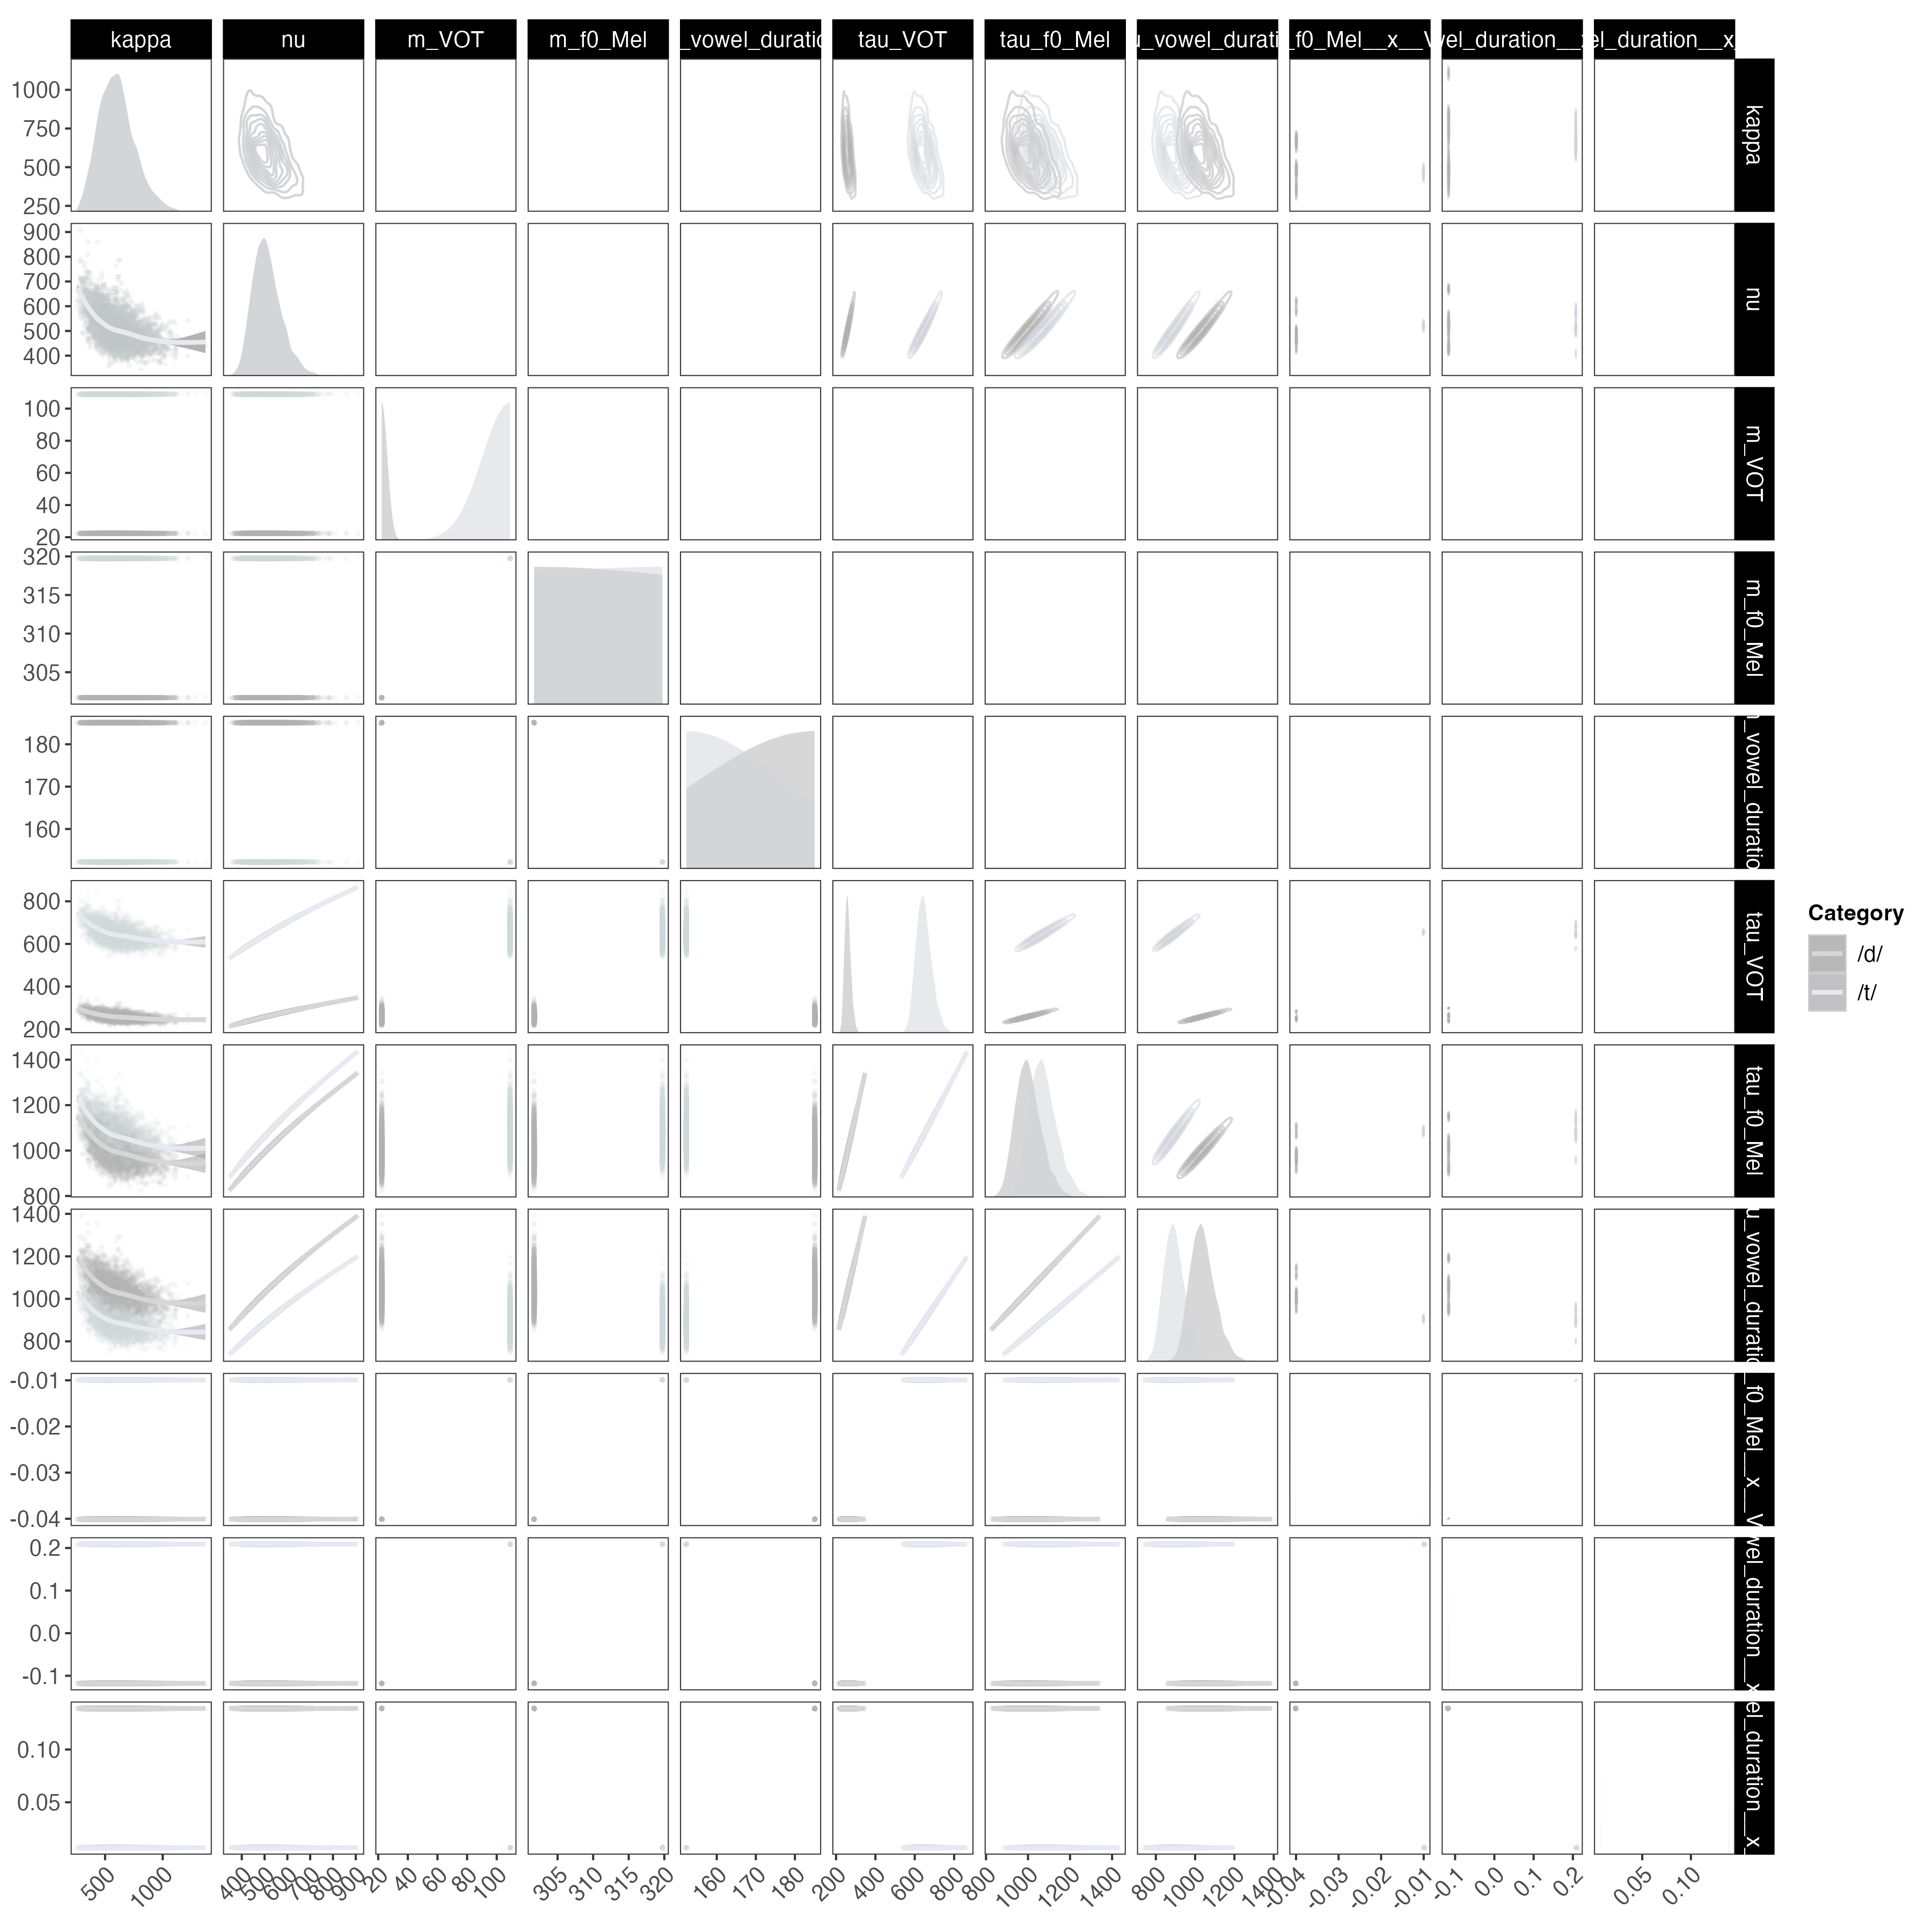
\includegraphics[width=1\linewidth]{../figures/ideal-adaptor-parameter-correlations} 

}

\caption{Marginal distributions (\textbf{panels on diagonal}), pairwise scatter plots (\textbf{lower off-diagonal}), and pairwise densities (\textbf{upper off-diagonals}) of parameters inferred for the ideal adaptor. Both latent and observed parameters are shown.}\label{fig:ideal-adaptor-parameter-correlations}
\end{figure}



\begin{figure}[H]

{\centering 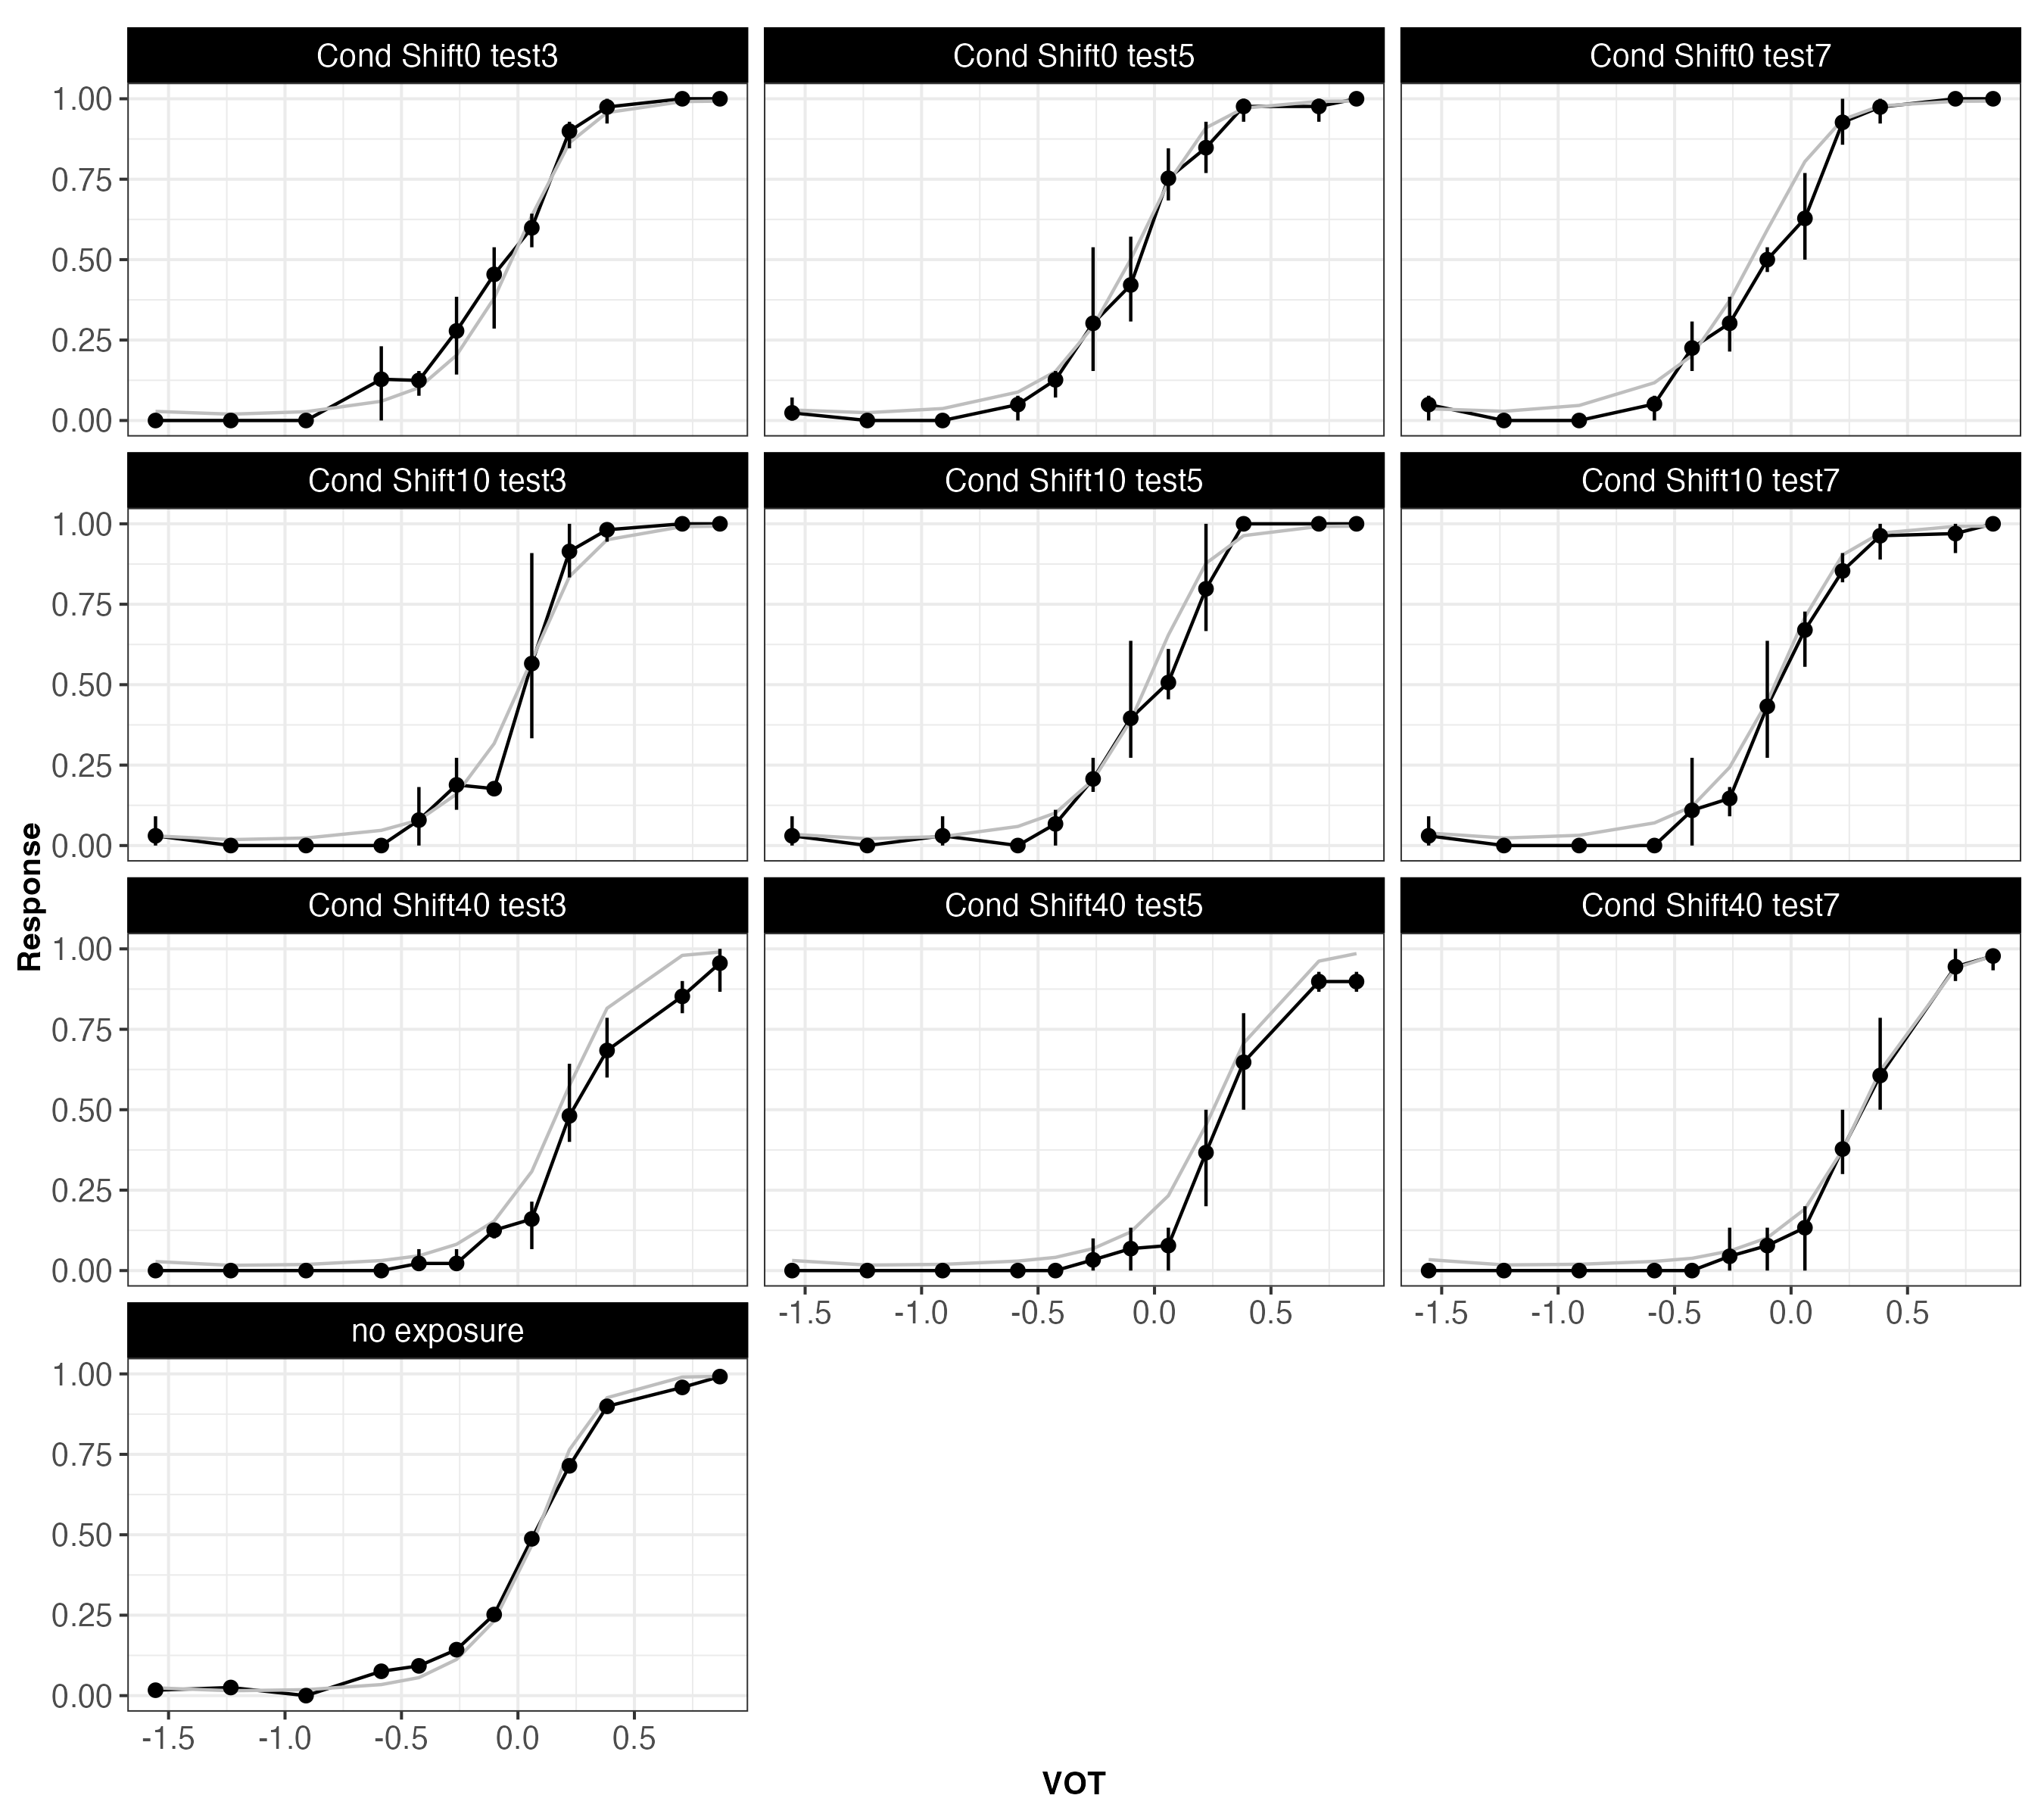
\includegraphics[width=1\linewidth]{../figures/ideal-adaptor-fitconditions-blocks} 

}

\caption{Comparing predictions of the ideal adaptor against participants' responses. Predicted and observed probability of ``t''-responses at each tested VOT for each combination of exposure condition and block.}\label{fig:ideal-adaptor-test-categorization}
\end{figure}



\begin{figure}[H]

{\centering 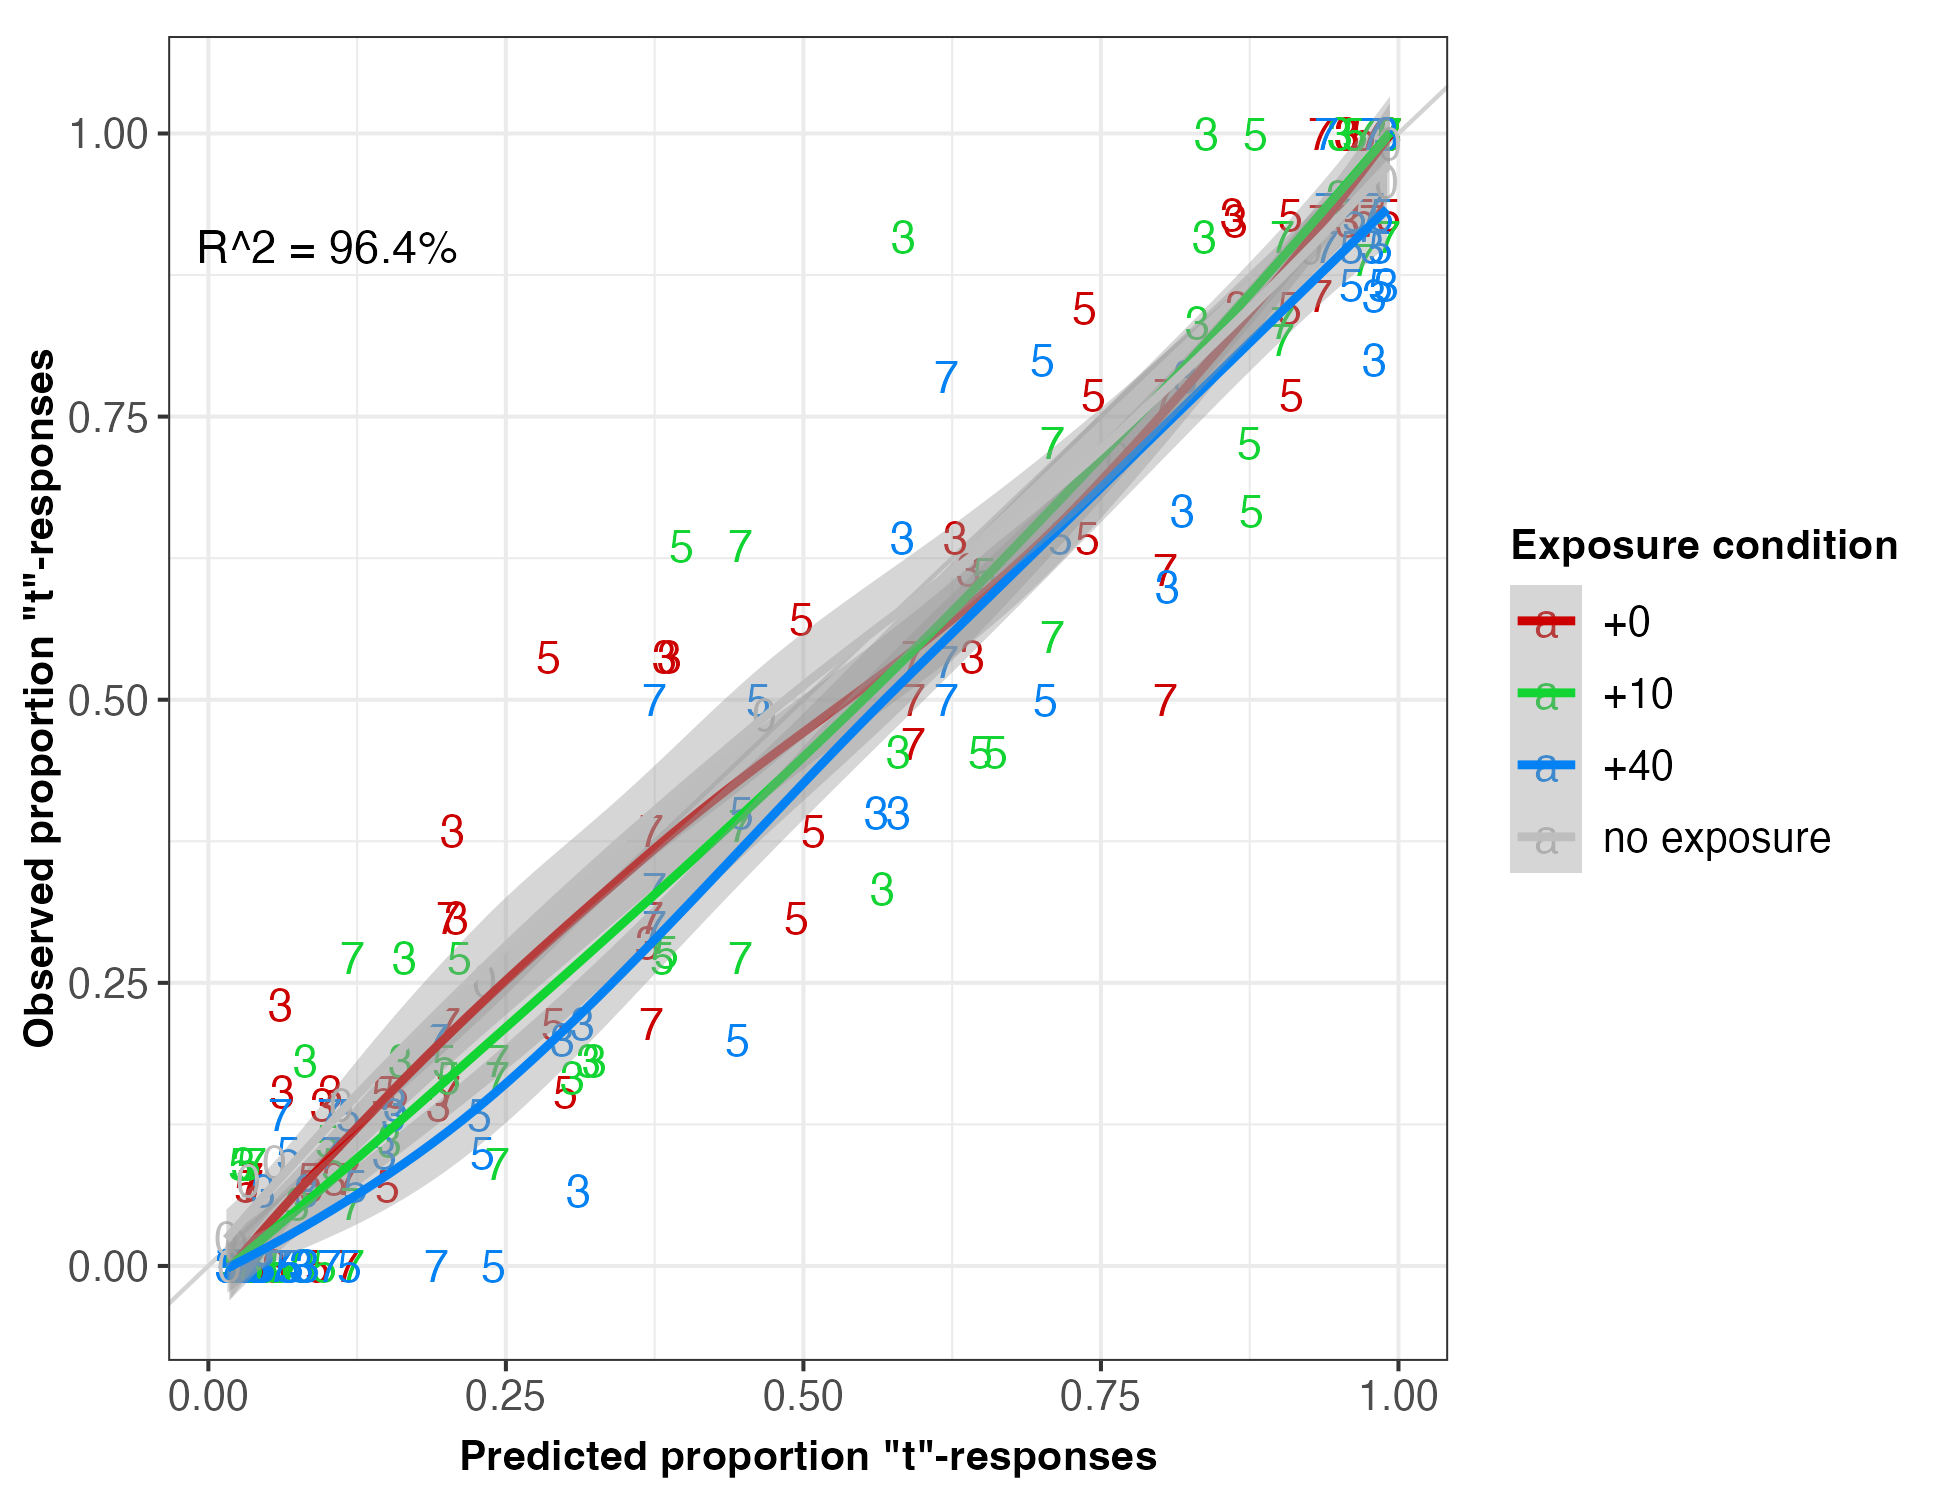
\includegraphics[width=1\linewidth]{../figures/ideal-adaptor-fit} 

}

\caption{Same as Figure \ref{fig:ideal-adaptor-test-categorization} but combining data across all conditions and blocks, in order to summarize the correlation between model predictions and participants' responses.}\label{fig:ideal-adaptor-test-categorization-r2}
\end{figure}

\printbibliography
\erefsection

\section{Session Info}\label{session-info}

\begin{verbatim}
## - Session info ---------------------------------------------------------------------------------------------------------------------------------------------------------------------------------------
##  setting  value
##  version  R version 4.4.1 (2024-06-14)
##  os       macOS Sonoma 14.6.1
##  system   aarch64, darwin20
##  ui       X11
##  language (EN)
##  collate  en_US.UTF-8
##  ctype    en_US.UTF-8
##  tz       Europe/Stockholm
##  date     2024-10-14
##  pandoc   3.1.11 @ /Applications/RStudio.app/Contents/Resources/app/quarto/bin/tools/aarch64/ (via rmarkdown)
## 
## - Packages -------------------------------------------------------------------------------------------------------------------------------------------------------------------------------------------
##  package         * version    date (UTC) lib source
##  abind             1.4-5      2016-07-21 [1] CRAN (R 4.4.0)
##  arrayhelpers      1.1-0      2020-02-04 [1] CRAN (R 4.4.0)
##  assertthat      * 0.2.1      2019-03-21 [1] CRAN (R 4.4.0)
##  av                0.9.1      2024-08-16 [1] CRAN (R 4.4.0)
##  backports         1.5.0      2024-05-23 [1] CRAN (R 4.4.0)
##  base64enc         0.1-3      2015-07-28 [1] CRAN (R 4.4.0)
##  bayesplot         1.11.1     2024-02-15 [1] CRAN (R 4.4.0)
##  bit               4.0.5      2022-11-15 [1] CRAN (R 4.4.0)
##  bit64             4.0.5      2020-08-30 [1] CRAN (R 4.4.0)
##  bookdown          0.40       2024-07-02 [1] CRAN (R 4.4.0)
##  boot              1.3-30     2024-02-26 [1] CRAN (R 4.4.1)
##  bridgesampling    1.1-2      2021-04-16 [1] CRAN (R 4.4.0)
##  brms            * 2.21.0     2024-03-20 [1] CRAN (R 4.4.0)
##  Brobdingnag       1.2-9      2022-10-19 [1] CRAN (R 4.4.0)
##  broom             1.0.6      2024-05-17 [1] CRAN (R 4.4.0)
##  broom.mixed     * 0.2.9.5    2024-04-01 [1] CRAN (R 4.4.0)
##  cachem            1.1.0      2024-05-16 [1] CRAN (R 4.4.0)
##  checkmate         2.3.2      2024-07-29 [1] CRAN (R 4.4.0)
##  class             7.3-22     2023-05-03 [1] CRAN (R 4.4.1)
##  classInt          0.4-10     2023-09-05 [1] CRAN (R 4.4.0)
##  cli               3.6.3      2024-06-21 [1] CRAN (R 4.4.0)
##  clue              0.3-65     2023-09-23 [1] CRAN (R 4.4.0)
##  cluster           2.1.6      2023-12-01 [1] CRAN (R 4.4.1)
##  coda              0.19-4.1   2024-01-31 [1] CRAN (R 4.4.0)
##  codetools         0.2-20     2024-03-31 [1] CRAN (R 4.4.1)
##  colorspace        2.1-1      2024-07-26 [1] CRAN (R 4.4.0)
##  cowplot           1.1.3      2024-01-22 [1] CRAN (R 4.4.0)
##  crayon            1.5.3      2024-06-20 [1] CRAN (R 4.4.0)
##  curl              5.2.2      2024-08-26 [1] CRAN (R 4.4.1)
##  data.table        1.16.0     2024-08-27 [1] CRAN (R 4.4.1)
##  DBI               1.2.3      2024-06-02 [1] CRAN (R 4.4.0)
##  devtools          2.4.5      2022-10-11 [1] CRAN (R 4.4.0)
##  digest            0.6.37     2024-08-19 [1] CRAN (R 4.4.1)
##  diptest         * 0.77-1     2024-04-10 [1] CRAN (R 4.4.0)
##  distributional    0.4.0      2024-02-07 [1] CRAN (R 4.4.0)
##  dplyr           * 1.1.4      2023-11-17 [1] CRAN (R 4.4.0)
##  e1071             1.7-14     2023-12-06 [1] CRAN (R 4.4.0)
##  ellipse           0.5.0      2023-07-20 [1] CRAN (R 4.4.0)
##  ellipsis          0.3.2      2021-04-29 [1] CRAN (R 4.4.0)
##  evaluate          0.24.0     2024-06-10 [1] CRAN (R 4.4.0)
##  extraDistr        1.10.0     2023-11-30 [1] CRAN (R 4.4.0)
##  fansi             1.0.6      2023-12-08 [1] CRAN (R 4.4.0)
##  farver            2.1.2      2024-05-13 [1] CRAN (R 4.4.0)
##  fastmap           1.2.0      2024-05-15 [1] CRAN (R 4.4.0)
##  fBasics           4041.97    2024-08-19 [1] CRAN (R 4.4.1)
##  forcats         * 1.0.0      2023-01-29 [1] CRAN (R 4.4.0)
##  foreach           1.5.2      2022-02-02 [1] CRAN (R 4.4.0)
##  foreign           0.8-86     2023-11-28 [1] CRAN (R 4.4.1)
##  Formula           1.2-5      2023-02-24 [1] CRAN (R 4.4.0)
##  fs                1.6.4      2024-04-25 [1] CRAN (R 4.4.0)
##  furrr           * 0.3.1      2022-08-15 [1] CRAN (R 4.4.0)
##  future          * 1.34.0     2024-07-29 [1] CRAN (R 4.4.0)
##  generics          0.1.3      2022-07-05 [1] CRAN (R 4.4.0)
##  gganimate         1.0.9      2024-02-27 [1] CRAN (R 4.4.0)
##  ggdist            3.3.2      2024-03-05 [1] CRAN (R 4.4.0)
##  ggforce         * 0.4.2      2024-02-19 [1] CRAN (R 4.4.0)
##  ggnewscale      * 0.5.0      2024-07-19 [1] CRAN (R 4.4.0)
##  ggplot2         * 3.5.1      2024-04-23 [1] CRAN (R 4.4.0)
##  ggridges          0.5.6      2024-01-23 [1] CRAN (R 4.4.0)
##  ggstance        * 0.3.7      2024-04-05 [1] CRAN (R 4.4.0)
##  ggtext          * 0.1.2      2022-09-16 [1] CRAN (R 4.4.0)
##  gifski            1.12.0-2   2023-08-12 [1] CRAN (R 4.4.0)
##  globals           0.16.3     2024-03-08 [1] CRAN (R 4.4.0)
##  glue              1.7.0      2024-01-09 [1] CRAN (R 4.4.0)
##  gridExtra         2.3        2017-09-09 [1] CRAN (R 4.4.0)
##  gridtext          0.1.5      2022-09-16 [1] CRAN (R 4.4.0)
##  gtable            0.3.5      2024-04-22 [1] CRAN (R 4.4.0)
##  here            * 1.0.1      2020-12-13 [1] CRAN (R 4.4.0)
##  Hmisc             5.1-3      2024-05-28 [1] CRAN (R 4.4.0)
##  hms               1.1.3      2023-03-21 [1] CRAN (R 4.4.0)
##  htmlTable         2.4.3      2024-07-21 [1] CRAN (R 4.4.0)
##  htmltools         0.5.8.1    2024-04-04 [1] CRAN (R 4.4.0)
##  htmlwidgets       1.6.4      2023-12-06 [1] CRAN (R 4.4.0)
##  httpuv            1.6.15     2024-03-26 [1] CRAN (R 4.4.0)
##  inline            0.3.19     2021-05-31 [1] CRAN (R 4.4.0)
##  isoband           0.2.7      2022-12-20 [1] CRAN (R 4.4.0)
##  iterators         1.0.14     2022-02-05 [1] CRAN (R 4.4.0)
##  jsonlite          1.8.8      2023-12-04 [1] CRAN (R 4.4.0)
##  kableExtra      * 1.4.0      2024-01-24 [1] CRAN (R 4.4.0)
##  KernSmooth        2.23-24    2024-05-17 [1] CRAN (R 4.4.1)
##  knitr             1.48       2024-07-07 [1] CRAN (R 4.4.0)
##  labeling          0.4.3      2023-08-29 [1] CRAN (R 4.4.0)
##  LaplacesDemon     16.1.6     2021-07-09 [1] CRAN (R 4.4.0)
##  later             1.3.2      2023-12-06 [1] CRAN (R 4.4.0)
##  latexdiffr      * 0.2.0      2024-02-16 [1] CRAN (R 4.4.0)
##  lattice           0.22-6     2024-03-20 [1] CRAN (R 4.4.1)
##  lifecycle         1.0.4      2023-11-07 [1] CRAN (R 4.4.0)
##  linguisticsdown * 1.2.0      2019-03-01 [1] CRAN (R 4.4.0)
##  listenv           0.9.1      2024-01-29 [1] CRAN (R 4.4.0)
##  lme4              1.1-35.5   2024-07-03 [1] CRAN (R 4.4.0)
##  loo               2.8.0      2024-07-03 [1] CRAN (R 4.4.0)
##  lpSolve           5.6.20     2023-12-10 [1] CRAN (R 4.4.0)
##  lubridate       * 1.9.3      2023-09-27 [1] CRAN (R 4.4.0)
##  magick          * 2.8.4      2024-07-14 [1] CRAN (R 4.4.0)
##  magrittr        * 2.0.3      2022-03-30 [1] CRAN (R 4.4.0)
##  MASS              7.3-60.2   2024-04-26 [1] CRAN (R 4.4.1)
##  Matrix            1.7-0      2024-04-26 [1] CRAN (R 4.4.1)
##  matrixStats       1.4.0      2024-09-04 [1] CRAN (R 4.4.1)
##  memoise           2.0.1      2021-11-26 [1] CRAN (R 4.4.0)
##  mgcv              1.9-1      2023-12-21 [1] CRAN (R 4.4.1)
##  mime              0.12       2021-09-28 [1] CRAN (R 4.4.0)
##  miniUI            0.1.1.1    2018-05-18 [1] CRAN (R 4.4.0)
##  minqa             1.2.8      2024-08-17 [1] CRAN (R 4.4.0)
##  modeest           2.4.0      2019-11-18 [1] CRAN (R 4.4.0)
##  munsell           0.5.1      2024-04-01 [1] CRAN (R 4.4.0)
##  MVBeliefUpdatr  * 0.0.1.0010 2024-05-11 [1] Github (hlplab/MVBeliefUpdatr@79ce502)
##  mvtnorm           1.3-1      2024-09-03 [1] CRAN (R 4.4.1)
##  nlme              3.1-164    2023-11-27 [1] CRAN (R 4.4.1)
##  nloptr            2.1.1      2024-06-25 [1] CRAN (R 4.4.0)
##  nnet              7.3-19     2023-05-03 [1] CRAN (R 4.4.1)
##  papaja          * 0.1.1.9001 2024-10-02 [1] Github (crsh/papaja@bd1aa4a)
##  parallelly        1.38.0     2024-07-27 [1] CRAN (R 4.4.0)
##  patchwork       * 1.2.0      2024-01-08 [1] CRAN (R 4.4.0)
##  phonR           * 1.0-7      2016-08-25 [1] CRAN (R 4.4.0)
##  pillar            1.9.0      2023-03-22 [1] CRAN (R 4.4.0)
##  pkgbuild          1.4.4      2024-03-17 [1] CRAN (R 4.4.0)
##  pkgconfig         2.0.3      2019-09-22 [1] CRAN (R 4.4.0)
##  pkgload           1.4.0      2024-06-28 [1] CRAN (R 4.4.0)
##  plyr              1.8.9      2023-10-02 [1] CRAN (R 4.4.0)
##  png               0.1-8      2022-11-29 [1] CRAN (R 4.4.0)
##  polyclip          1.10-7     2024-07-23 [1] CRAN (R 4.4.0)
##  posterior       * 1.6.0      2024-07-03 [1] CRAN (R 4.4.0)
##  prettyunits       1.2.0      2023-09-24 [1] CRAN (R 4.4.0)
##  profvis           0.3.8      2023-05-02 [1] CRAN (R 4.4.0)
##  progress          1.2.3      2023-12-06 [1] CRAN (R 4.4.0)
##  promises          1.3.0      2024-04-05 [1] CRAN (R 4.4.0)
##  proxy             0.4-27     2022-06-09 [1] CRAN (R 4.4.0)
##  purrr           * 1.0.2      2023-08-10 [1] CRAN (R 4.4.0)
##  QuickJSR          1.3.1      2024-07-14 [1] CRAN (R 4.4.0)
##  R6                2.5.1      2021-08-19 [1] CRAN (R 4.4.0)
##  rbibutils         2.2.16     2023-10-25 [1] CRAN (R 4.4.0)
##  RColorBrewer      1.1-3      2022-04-03 [1] CRAN (R 4.4.0)
##  Rcpp            * 1.0.13     2024-07-17 [1] CRAN (R 4.4.0)
##  RcppParallel      5.1.9      2024-08-19 [1] CRAN (R 4.4.1)
##  Rdpack            2.6.1      2024-08-06 [1] CRAN (R 4.4.0)
##  readr           * 2.1.5      2024-01-10 [1] CRAN (R 4.4.0)
##  remotes           2.5.0      2024-03-17 [1] CRAN (R 4.4.0)
##  reshape2          1.4.4      2020-04-09 [1] CRAN (R 4.4.0)
##  rlang           * 1.1.4      2024-06-04 [1] CRAN (R 4.4.0)
##  rmarkdown         2.28       2024-08-17 [1] CRAN (R 4.4.0)
##  rmutil            1.1.10     2022-10-27 [1] CRAN (R 4.4.0)
##  rpart             4.1.23     2023-12-05 [1] CRAN (R 4.4.1)
##  rprojroot         2.0.4      2023-11-05 [1] CRAN (R 4.4.0)
##  rsample         * 1.2.1      2024-03-25 [1] CRAN (R 4.4.0)
##  rstan             2.32.6     2024-03-05 [1] CRAN (R 4.4.0)
##  rstantools        2.4.0      2024-01-31 [1] CRAN (R 4.4.0)
##  rstudioapi        0.16.0     2024-03-24 [1] CRAN (R 4.4.0)
##  scales            1.3.0      2023-11-28 [1] CRAN (R 4.4.0)
##  sessioninfo       1.2.2      2021-12-06 [1] CRAN (R 4.4.0)
##  sf                1.0-17     2024-09-06 [1] CRAN (R 4.4.1)
##  shiny             1.9.1      2024-08-01 [1] CRAN (R 4.4.0)
##  spatial           7.3-17     2023-07-20 [1] CRAN (R 4.4.1)
##  stable            1.1.6      2022-03-02 [1] CRAN (R 4.4.0)
##  stabledist        0.7-2      2024-08-17 [1] CRAN (R 4.4.0)
##  StanHeaders       2.32.10    2024-07-15 [1] CRAN (R 4.4.0)
##  statip            0.2.3      2019-11-17 [1] CRAN (R 4.4.0)
##  stringi           1.8.4      2024-05-06 [1] CRAN (R 4.4.0)
##  stringr         * 1.5.1      2023-11-14 [1] CRAN (R 4.4.0)
##  supunsup        * 0.2.0      2024-09-07 [1] Github (kleinschmidt/phonetic-sup-unsup@5c51177)
##  svglite           2.1.3      2023-12-08 [1] CRAN (R 4.4.0)
##  svUnit            1.0.6      2021-04-19 [1] CRAN (R 4.4.0)
##  systemfonts       1.1.0      2024-05-15 [1] CRAN (R 4.4.0)
##  tensorA           0.36.2.1   2023-12-13 [1] CRAN (R 4.4.0)
##  tibble          * 3.2.1      2023-03-20 [1] CRAN (R 4.4.0)
##  tidybayes       * 3.0.6      2023-08-12 [1] CRAN (R 4.4.0)
##  tidyr           * 1.3.1      2024-01-24 [1] CRAN (R 4.4.0)
##  tidyselect        1.2.1      2024-03-11 [1] CRAN (R 4.4.0)
##  tidyverse       * 2.0.0      2023-02-22 [1] CRAN (R 4.4.0)
##  timechange        0.3.0      2024-01-18 [1] CRAN (R 4.4.0)
##  timeDate          4032.109   2023-12-14 [1] CRAN (R 4.4.0)
##  timeSeries        4032.109   2024-01-14 [1] CRAN (R 4.4.0)
##  tinylabels      * 0.2.4      2023-09-02 [1] CRAN (R 4.4.0)
##  transformr        0.1.5      2024-02-26 [1] CRAN (R 4.4.0)
##  tweenr            2.0.3      2024-02-26 [1] CRAN (R 4.4.0)
##  tzdb              0.4.0      2023-05-12 [1] CRAN (R 4.4.0)
##  units             0.8-5      2023-11-28 [1] CRAN (R 4.4.0)
##  urlchecker        1.0.1      2021-11-30 [1] CRAN (R 4.4.0)
##  usethis           3.0.0      2024-07-29 [1] CRAN (R 4.4.0)
##  utf8              1.2.4      2023-10-22 [1] CRAN (R 4.4.0)
##  V8                5.0.1      2024-09-20 [1] CRAN (R 4.4.1)
##  vctrs             0.6.5      2023-12-01 [1] CRAN (R 4.4.0)
##  viridis           0.6.5      2024-01-29 [1] CRAN (R 4.4.0)
##  viridisLite       0.4.2      2023-05-02 [1] CRAN (R 4.4.0)
##  vroom             1.6.5      2023-12-05 [1] CRAN (R 4.4.0)
##  webshot         * 0.5.5      2023-06-26 [1] CRAN (R 4.4.0)
##  withr             3.0.1      2024-07-31 [1] CRAN (R 4.4.0)
##  xfun              0.47       2024-08-17 [1] CRAN (R 4.4.0)
##  xml2              1.3.6      2023-12-04 [1] CRAN (R 4.4.0)
##  xtable            1.8-4      2019-04-21 [1] CRAN (R 4.4.0)
##  yaml              2.3.10     2024-07-26 [1] CRAN (R 4.4.0)
## 
##  [1] /Library/Frameworks/R.framework/Versions/4.4-arm64/Resources/library
## 
## ------------------------------------------------------------------------------------------------------------------------------------------------------------------------------------------------------
\end{verbatim}


\printbibliography

\end{document}
